\documentclass{article}
% ====================================
% PACKAGES
% ====================================

\usepackage{arxiv}
\usepackage[utf8]{inputenc} % allow utf-8 input
\usepackage[T1]{fontenc}    % use 8-bit T1 fonts
\usepackage{microtype}      % microtypography
\usepackage{amsfonts}
\usepackage{amsmath}
\usepackage{bm}
\usepackage[hidelinks]{hyperref}
\usepackage{graphicx}
\usepackage{mathtools}
\usepackage{enumitem}
\usepackage{setspace}
\usepackage{subcaption}
\usepackage[dvipsnames]{xcolor}
\usepackage{color}
\graphicspath{{figures/}}
\usepackage{upgreek}
\usepackage{cases}
\usepackage{arydshln}
\usepackage{wrapfig}
\usepackage{blkarray}
\usepackage{enumitem}
\usepackage{textcomp}  % silence gensym warnings
\usepackage{gensymb}  % for \degree
\usepackage{siunitx}  % for \num
%\sisetup{output-exponent-marker=\ensuremath{\mathrm{e}}}
\usepackage{booktabs}
\usepackage{longtable}
\usepackage[export]{adjustbox}% http://ctan.org/pkg/adjustbox
\usepackage[ruled,vlined]{algorithm2e}

%% ADDED BY LAURENE - DOUBLE SPACE
%\usepackage{setspace}
%%\onehalfspacing
%\doublespacing

% ====================================
% COMMANDS
% ====================================

\newcommand{\figref}[1]{Figure~\ref{fig:#1}}
\newcommand{\tabref}[1]{Table~\ref{tab:#1}}
%\newcommand{\secref}[1]{Section~\ref{sec:#1}}
\newcommand{\secref}[1]{\S\ref{sec:#1}}
%\newcommand{\eqnref}[1]{(\ref{eqn:#1})}
\newcommand{\eqnref}[1]{\eqref{eqn:#1}}
%\newcommand{\eqnref}[1]{equation~\eqref{eqn:#1}}

% comments
\newcommand{\todo}[1]{{\color[rgb]{.6,.1,.6}{#1}}}
\newcommand{\banjac}[1]{{\color[rgb]{.3,.5,.9}{#1}}}
\newcommand{\lau}[1]{{\textcolor{OliveGreen}{#1}}}
\newcommand{\mdeff}[1]{{\color[rgb]{.8,.3,.2}{#1}}}

% ====================================
% MATH
% ====================================

%\newcommand\argmin[1]{\underset{#1}{\arg\;\min}}
\DeclareMathOperator*{\argmin}{arg\,min}

\newcommand\R{\mathbb{R}}
\newcommand\Rot{\mathbf{R}}
\newcommand\T{\mathbf{T}}
\newcommand\Or[0]{\mathrm{\mathbf{O}}}
\newcommand\SO[0]{\mathrm{\mathbf{SO}}}

\newcommand\x{\mathbf{x}}
\newcommand\p{\mathbf{p}}
\newcommand\f{\mathbf{f}}
\newcommand\G{\mathcal{G}}

\newcommand\bth[0]{{\boldsymbol{\theta}}}
\newcommand\bsx[0]{{\boldsymbol{x}}}

% ====================================
% TIKZ
% ====================================

\usepackage{tikz,pgfplots,pgfplotstable}
\usepgfplotslibrary{groupplots,fillbetween,colorbrewer,statistics}
\usetikzlibrary{intersections,calc,arrows,matrix,spy,pgfplots.statistics, pgfplots.colorbrewer}
\usepackage{color}
\definecolor{darkred}{rgb}{0.7,0,0}
\definecolor{darkgreen}{rgb}{0,0.5,0}
\definecolor{darkblue}{rgb}{0,0,0.7}
\definecolor{SkyBlue}{rgb}{0.53, 0.81, 0.92}
\pgfplotsset{compat=1.5.1, cycle list/Set1-3}
\usepackage{tikz-3dplot}


%\renewcommand{\headeright}{Technical Report}
%\renewcommand{\undertitle}{Technical Report}
\renewcommand{\headeright}{}
\renewcommand{\undertitle}{}

\author{
    \href{https://orcid.org/0000-0001-7373-4150}{
\includegraphics[scale=0.06]{orcid}\hspace{1mm}}Jelena Banjac, \href{https://orcid.org/0000-0001-9834-7755}{
\includegraphics[scale=0.06]{orcid}\hspace{1mm}}Laurène Donati, \href{https://orcid.org/0000-0002-6028-9024}{
\includegraphics[scale=0.06]{orcid}\hspace{1mm}}Michaël Defferrard \\
    EPFL, Switzerland \\
    \texttt{\{jelena.banjac,laurene.donati,michael.defferrard\}@epfl.ch}
}

\date{}
\title{Learning to recover orientations from projections in single-particle cryo-EM}

%\title{Learning to recover the orientations of projections in single-particle cryo-EM}
%\title{Learning to recover the orientation of cryo-EM projections}
%\title{Recovering the orientation of cryo-EM projections from learned distance estimation}
%\title{Recovery of Orientations in SPA: Learning from Projections}
%\title{Learning to recover orientations from projections}
%\title{3D Poses Recovery in Single-Particle Cryo-EM from Learned Pairwise Projection Distances}
% keywords: learning, protein imaging/reconstruction (why/goal), (single-particle) Cryo-EM, SPA

%%%%%%%%%%%%%%%%%%%%%%%%%%%%%%%%%%%%%%%%%%%%%%%%%%%%%%%%%%%%%%%%%%%%

\begin{document}

\maketitle

\begin{abstract}
    A major challenge in single-particle cryo-electron microscopy (cryo-EM) is that the orientations adopted by the 3D particles prior to imaging are unknown; yet, their knowledge is essential for high-resolution reconstruction.
    We present a method to recover these orientations directly from the acquired set of 2D projections. Our approach consists of two steps: (i) the estimation of the relative distances between numerous pairs of projections, and (ii) the recovery of the absolute orientation of each projection from these distances.
    % absolute orientations vs relative distances?
    For step (i), the pairwise distance estimator is a Siamese neural network trained on synthetic cryo-EM projections from resolved bio-structures.
    For step (ii), the orientations are recovered by minimizing an appropriate loss function.
    Experimental results show that \lau{put here the latest results situation. %the quality of the recovered orientations strongly depends on the quality of the estimated distances.
    While not yet up to state-of-the art ..., distance estimation is robust to perturbations (adapt).}
    Overall, the orientations recovered from simulated noisy projections are within \todo{10\degree} of the true orientations.
    Our code is available at \url{https://github.com/JelenaBanjac/protein-reconstruction}.
\end{abstract}


\section{Introduction}

Single-particle cryo-electron microscopy (cryo-EM) has revolutionized the field of structural biology over the last decades~\cite{dubochet1988cryo, frank2006three,chap0-nat2015MethodYear}. The use of electron beams to image ice-embedded samples has permitted the recovery of 3D bio-structures at unprecedented resolution. This advent of atomic-resolution cryo-EM has had a tremendous impact in biomedical research, providing invaluable insights into the biological processes that underlie many current diseases.

In single-particle cryo-EM, every 3D particle adopt a random orientation in the ice layer before being imaged with parallel beams of electrons.
Hence, the projection geometry associated to each acquired 2D projection (\figref{imaging-geometry}) is unknown. Yet, this knowledge is essential for the tomographic reconstruction of bio-structures~\cite{Natterer2001mathematics}.

\tdplotsetmaincoords{60}{110}
\pgfmathsetmacro{\rvec}{.8}
\pgfmathsetmacro{\thetavec}{30}
\pgfmathsetmacro{\phivec}{60}
\begin{figure}
\centering
\begin{subfigure}[t]{0.35\linewidth}
    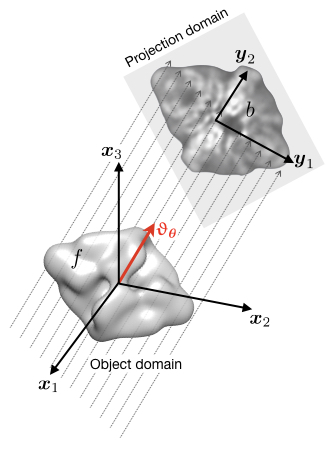
\includegraphics[width=\linewidth]{figures/imaging_geometry}
\end{subfigure}
\quad
\begin{tikzpicture}[scale=5,tdplot_main_coords]
    \coordinate (O) at (0,0,0);
    \draw[thick,->] (0,0,0) -- (1,0,0) node[anchor=north east]{$\bsx_1$};
    \draw[thick,->] (0,0,0) -- (0,1,0) node[anchor=north west]{$\bsx_2$};
    \draw[thick,->] (0,0,0) -- (0,0,1) node[anchor=south]{$\bsx_3$};
    \tdplotsetcoord{P}{\rvec}{\thetavec}{\phivec}
    \draw[-stealth,very thick,color=red] (O) -- (P);
    \draw[dashed, color=red] (O) -- (Pxy);
    \draw[dashed, color=red] (P) -- (Pxy);
    \tdplotdrawarc{(O)}{0.2}{0}{\phivec}{anchor=north}{$\theta_1$}
    \tdplotsetthetaplanecoords{\phivec}
    \tdplotdrawarc[tdplot_rotated_coords]{(0,0,0)}{0.5}{0}%
        {\thetavec}{anchor=south west}{$\theta_2$}
    \draw[dashed,tdplot_rotated_coords] (\rvec,0,0) arc (0:90:\rvec);
    \draw[dashed] (\rvec,0,0) arc (0:90:\rvec);
    \tdplotsetrotatedcoords{\phivec}{\thetavec}{0}
    \tdplotsetrotatedcoordsorigin{(P)}
    \draw[dashed,blue,tdplot_rotated_coords,-] (-.4,0,0)
        -- (.4,0,0) node[anchor=north west]{};
    \draw[dashed,blue,tdplot_rotated_coords,-] (0,-.4,0)
        -- (0,.4,0) node[anchor=west]{};
    \draw[blue,tdplot_rotated_coords,-]  (-.4,.4,0) -- (.4,.4,0)  -- (.4,-.4,0) -- (-.4,-.4,0) -- (-.4,.4,0)   node[anchor=north]{};
    \tdplotdrawarc[tdplot_rotated_coords]{(0,0,0)}{0.2}{0}%
        {30}{anchor=north west,color=black}{$\theta_3$}
    \tdplotsetrotatedcoords{\phivec}{\thetavec}{30}
    \draw[thick,tdplot_rotated_coords,->] (0,0,0)
        -- (.3,0,0) node[anchor=north west]{$\bsy_1$};
    \draw[thick,tdplot_rotated_coords,->] (0,0,0)
        -- (0,.3,0) node[anchor=west]{$\bsy_2$};
    \node[blue] at (0.4,0.45,1.2) {$\Omega_{\mathrm{2D}}$};
    \node[red] at (1.5,0.75,1.2) {$\bvth_{\bth}$};
    \tdplotsetrotatedthetaplanecoords{45}
\end{tikzpicture}
\caption{%
    % Goals: explain
    % * (i) what we mean by a projection and an orientation (the two most important objects of our paper), and
    % * (ii) how a projection (=integration through z in the new coordinate system) is made from a 3D volume.
    \lau{Easy solution if not enough time: just adapt this figure with the correct notations.}
    \mdeff{We should try to better convey the idea of a plane on the left figure. For example, there was a gray rectangle in the original image.}
    \todo{Imaging figure: $\Omega_{\mathrm{2D}}$ with 2D not italic. $\p$ in bold.}
    \todo{Method figure: A real protein in the middle, and some real projections on S². Similarly to the first figure in Jelena's notebook [1]. Curved lines would link the projections' centre, following the curvature of S². The goal is to explain that $d_q$ is the geodesic distance between orientations, and for readers to understand that given those distances, we can find the orientations back (up to a global orientation). The whole problem is then to infer the distances from the projections. (From subfig 1 it'll be apparent that S² is a subset of the space of orientations, missing in-plane rotations $\theta_3$.)}
    Geometry of the 3D imaging model.
    The 3D object in the coordinate system $(x_1,x_2, x_3)$ is imaged along the (unknown) projection direction $\bvth_{\bth}$ \mdeff{\textit{orientation} $q$?} to produce the 2D \textit{projection} $\p$ in the coordinate system $(y_1,y_2)$.
    The Euler angles $\bth=(\theta_1,\theta_2,\theta_3)\in\Omega_\bth$ represent the 3D rotation that maps the object coordinate system to the projection coordinate system.
    The angles $\theta_1$, $\theta_2$, and $\theta_3$, respectively correspond to the rotation, the tilt, and the in-plane rotation in the projection plane.
    The set $\Omega_{\mathrm{2D}}$ denotes the support of the projection.
    \mdeff{Is $\Omega_{\mathrm{2D}}$ a set? Not a vector space?}
}\label{fig:imaging-geometry}
\end{figure}

% RELATED WORKS
To handle this, a popular approach in single-particle cryo-EM is to alternatively refine the 3D structure and the estimation of the orientations~\cite{penczek1994ribosome,Baker1996,Dempster1977,sigworth1998maximum,scheres2012bayesian,zehni2020joint}. Unfortunately, the outcome of these iterative-refinement procedures is most often predicated on the quality of the initial \textit{ab initio} reconstruction, or, equivalently, on the initial estimation of the orientations~\cite{sorzano2006optimization,henderson2012outcome}.

Several methods have been designed to produce a first rough \textit{ab initio} structure for the refinement procedure~\cite{singer2020computational}. An early approach~\cite{kam1980reconstruction} proposed to reconstruct an initial structure such that the first few moments of the distribution of its theoretical measurements match the ones of its experimental projections. Since then, \textit{moment-matching} techniques have been refined and extended~\cite{salzman1990method,goncharov1988integral,sharon2019method}, \textit{e.g.}, to accommodate for non-uniform orientation configurations. However, they typically remain sensitive to error in data and can require relatively high computational complexity.  %If needs be for downside: relatively important computational complexity, and remain sensitive to error in data.

Another popular line of approach in single-particle cryo-EM  relies on the central-slice theorem, which relates the Fourier transform of a projection to a plane (orthogonal to the projection direction) in the Fourier transform of the 3D object~\cite{Natterer2001mathematics}. Hence, every two projections \textit{de facto} share a common 1D intersection in the 3D Fourier domain, and three projections theoretically suffice to define a coordinate system from which their orientations can be deduced~\cite{van1987angular}. Exploiting this principle, \textit{common-lines} methods aim at uniquely determining the orientations of each projections by identifying the common-lines between triplets of projections~\cite{penczek1994ribosome,mallick2006structure,singer2010detecting,wang2013orientation,greenberg2017common,pragier2019common}---a real technical challenge given the massive amount of noise in cryo-EM data. %If needs be for downside: sensitivity to high-noise levels, small particles, etc.

Alternatively, the  marginalized maximum likelihood (ML) formulation of the reconstruction problem---classically used for the iterative-refinement procedures themselves---can be minimized using stochastic gradient descents~\cite{punjani2017cryosparc}. This permits to avoid the need for an initial volume estimate, at the possible cost of greater convergence instability. More recently, the recovery of geometrical information from unknown view tomography of 2D point sources has been proposed~\cite{zehni2019distance}, but the extension to 3D cryo-EM tomography is not straightforward yet.

Hence, despite the many aforementioned advances, the task of providing a robust initial volume remains a notoriously arduous challenge in single-particle cryo-EM due to the high-dimensionality and strong ill-posedness of the underlying optimization problem.

%\mdeff{Content. (p1) Why is the general problem of protein reconstruction important and difficult. (p2) Short background on single-particle cryo-EM and how reconstruction is done. (p3) Previous work on orientation estimation (or initial structure estimation). If there's none (because people have researched other routes), state it and write why it's an interesting route to explore. How does it compare to initial rough structure estimation? Or whatever the other routes are. (p4) Our contribution on top of previous work.}

\section{Method}

% \lau{Lau: As far as I'm concerned, everything below before subsection 2.1 could also go at the end of the Introduction. Beyond the fact that it contains literature review and conceptual information that would go well in the intro, I find the current architecture of Section 2 a bit puzzling. First there is text to explain the methods and detail their intuition/key components, then there are three consecutive subsections that kind of do the same, but from a maths points of view. The aforementioned suggestion of putting the first text in the intro could solve this. Another possibility: put the descriptive texts in their corresponding sub-sections, so that those contain both the motivation and the maths. I'm open to further suggestions and suggestions ;-) }
% \mdeff{Indeed. The "Distance Learning" and "Orientation Recovery" paragraphs might go in their respective sub-sections. But I'd like to keep a high-level motivation of the whole method (the text linked to the second figure to appear alongside \figref{imaging-geometry}.}
% \lau{Fine for me.}
% \banjac{I moved the DE and OR to corresponding subsections. The short intro to methods I left here at the beginning of the section 2 (I didn't move it to intro). Let me know if you meant something different}

\begin{figure}
    \centering
    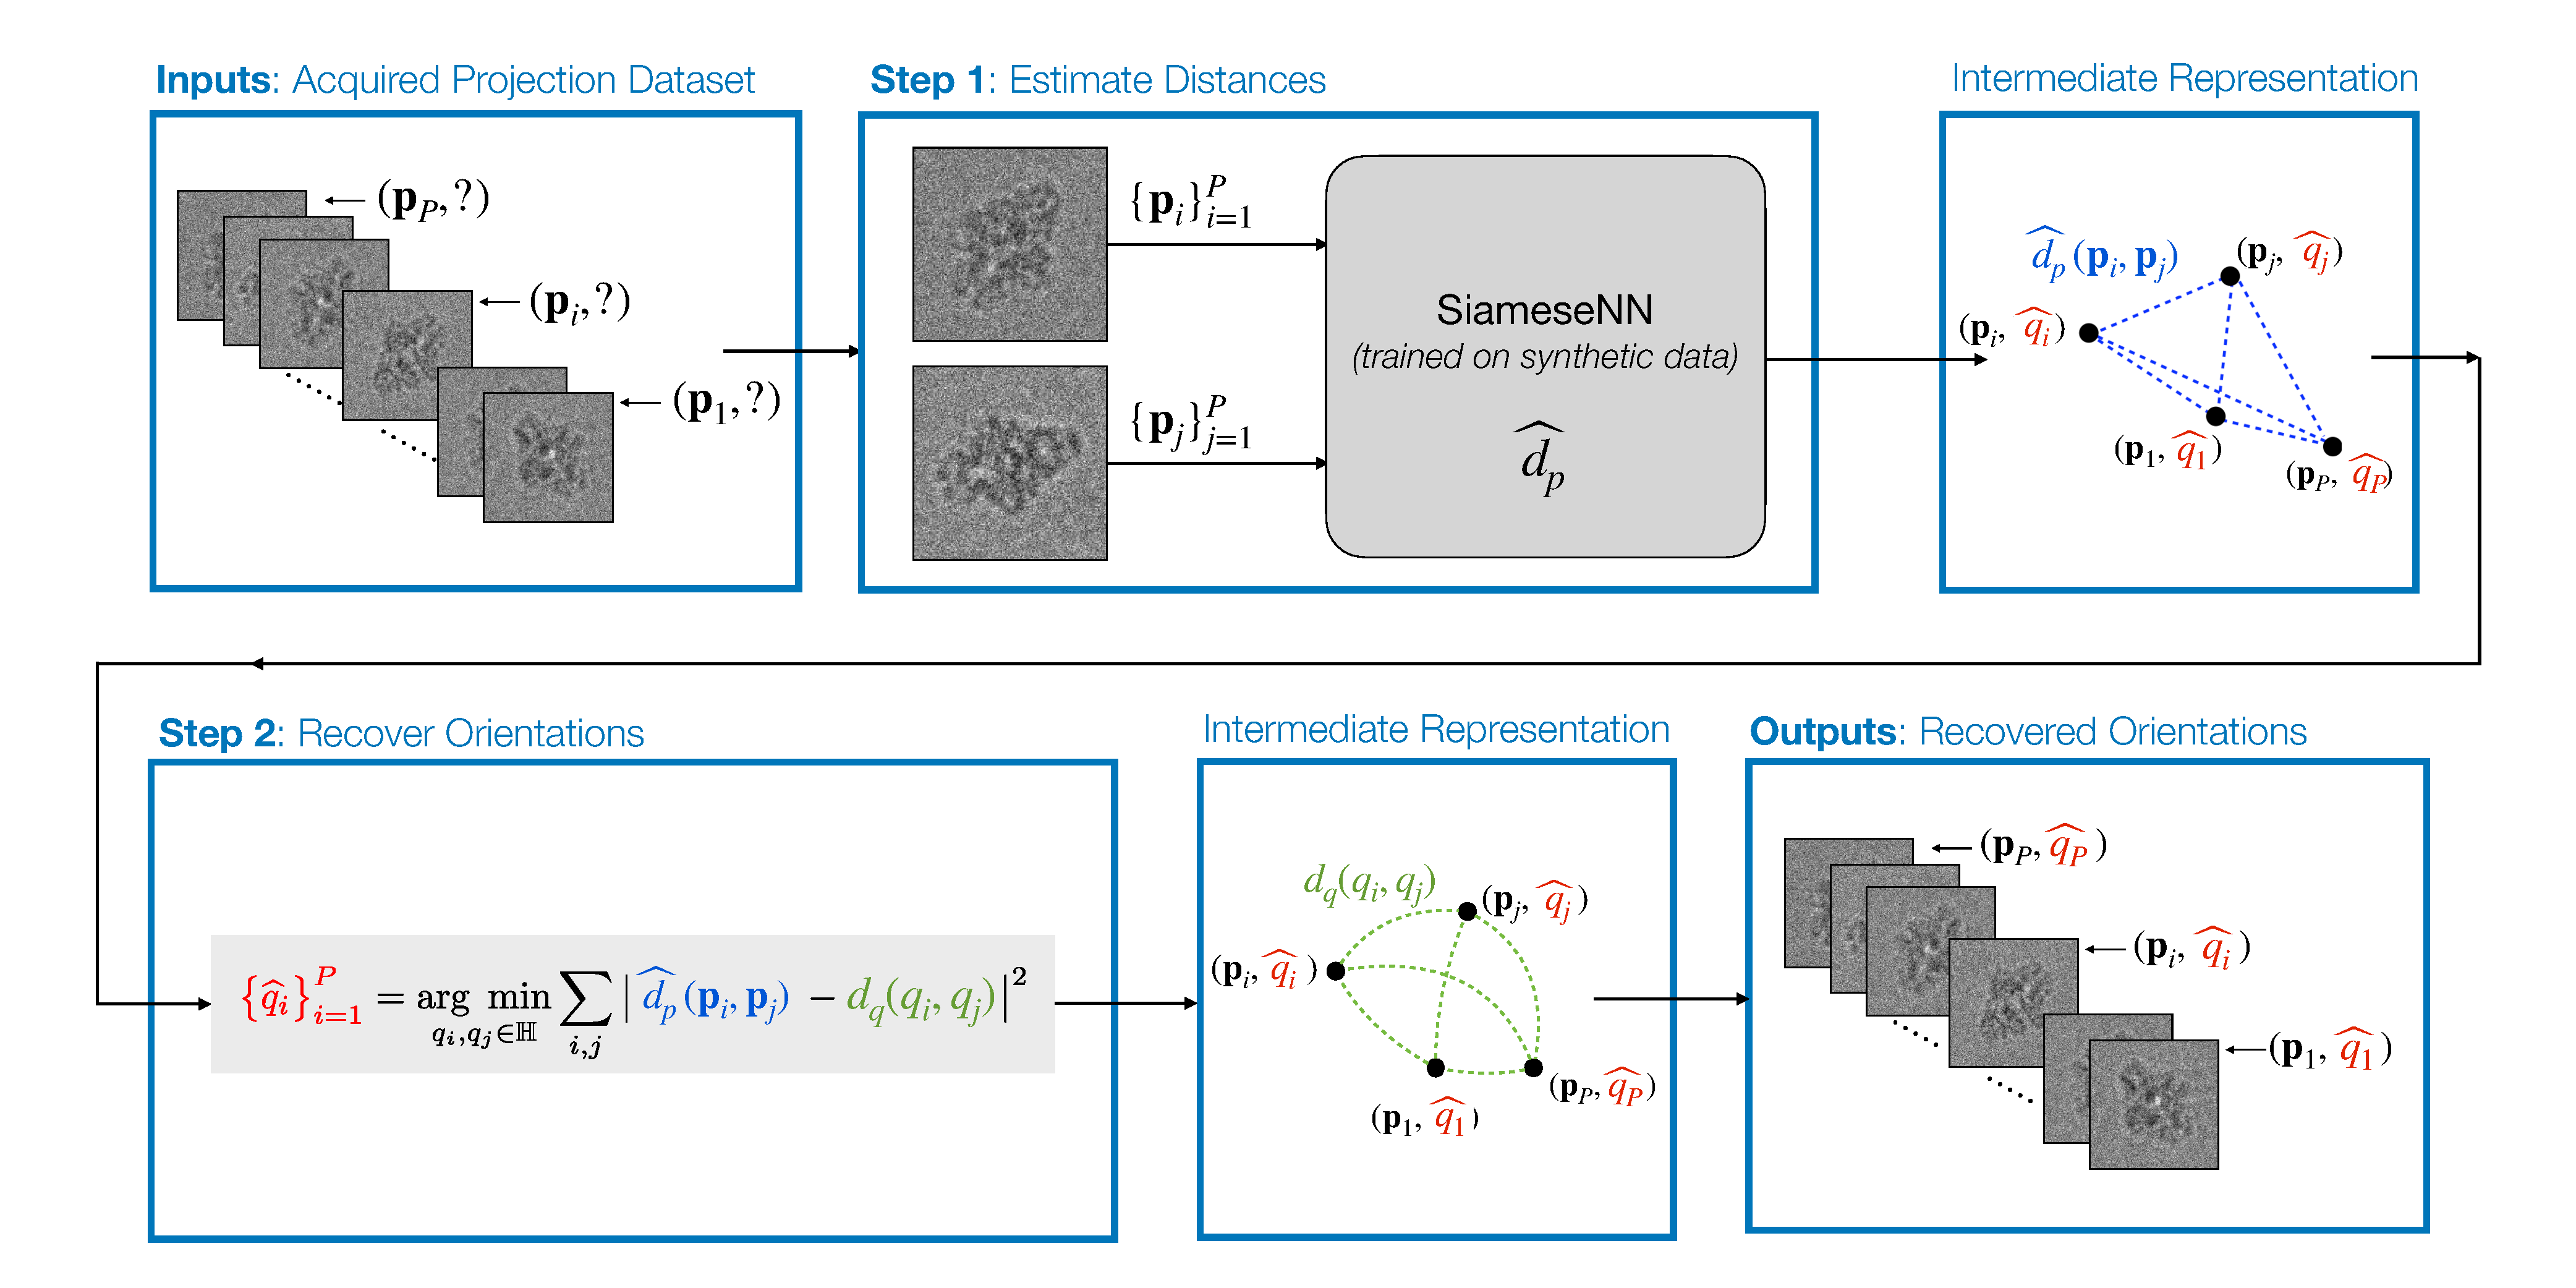
\includegraphics[width=\linewidth]{schematic_method_overview}
    \caption{%
        %\textbf{Method:}
        Our method consists of two steps.
        First, we estimate distances between pairs of projections.
        Second, we recover the orientation of each projection from these distances.
    }\label{fig:schematic:method-overview}
\end{figure}

Our approach relies on two observations (\figref{intuition-method}), yielding two steps (\figref{schematic:method-overview}).
First, the greater the similarity between two 2D projections $(\p_i, \p_j)$, the more likely they originated from two 3D particles that adopted close orientations $(q_i, q_j)$ in the ice layer prior to imaging;\footnote{Up to protein symmetries, which we discuss later.} this observation guides a number of applications in the field~\cite{frank2006three}.
% TODO: differences in orientation / distances
Hence, we aim to estimate differences in orientation $d_q(q_i, q_j)$ from the projections themselves as $\widehat{d_p}(\p_i, \p_j)$ (\secref{method:distance-learning}).
% where $\widehat{d_p}$ is learned from training data
Second, orientations are constrained by their relative differences.
Hence, from a set of projections $\{\p_k\}_{k=1}^P$, we aim to recover their orientations $\{\widehat{q_k}\}_{k=1}^P$ such that the induced distances $d_q(\widehat{q_i}, \widehat{q_j})$ are close to the estimated distances $\widehat{d_p}(\p_i, \p_j)$ (\secref{method:orientation-recovery}).
All in all, $d_q(q_i, q_j) \approx \widehat{d_p}(\p_i, \p_j) \approx d_q(\widehat{q_i}, \widehat{q_j})$, with equality if $\widehat{d_p}$ and $\{\widehat{q_k}\}_{k=1}^P$ are perfectly estimated.

%We propose to learn a function---parametrized as a neural network---to predict the relative orientation between two projections based on their similarity.
%This distance function then allows us to estimate, for any new projection dataset, the relative orientations between pairs of projections.

% Our method effectively (i) estimates a metric space, then (ii) embed/realize it in the space of 3D orientations, $\SO(3)$.

%Given sufficiently many and accurate estimations
%If the distances are exact geodesic distances between orientations, then orientation recovery will find a perfect realization of the metric space, with zero error.
%In practice, distances estimated from projections will only be a proxy of true distances.
%Experiment \secref{results:orientation-recovery:sensitivity} shows that a lower distance estimation error translates to a lower orientation recovery error.

%\subsection{Unit Quaternions and the Geodesic Distance}
%\subsection{Parameterization of orientations}
\subsection{Representation of orientations}\label{sec:method:orientation-representation}
%\subsection{Orientations and distances}\label{sec:method:orientation-representation}
%\subsection{Distance between orientations}
%\mdeff{Laurène: Which word is better: Representation or parameterization? Or something else, but we need consistency.}
%\lau{Both are fine. Personally, I use parametrization in my thesis, but we can settle on the other one.}
% representation of orientations, parameterization of rotation matrices

%The projection $\mathbf{P}_{\bth}$ in \eqnref{imaging-model} represents an integration through the 3D particle made by the beam of electrons.
The orientation of the 3D particle with respect to the microscope's detector plane is a rotation relative to a reference orientation (\figref{imaging-geometry}).
The group of all 3D rotations under composition is identified with $\SO(3)$, the group of $3 \times 3$ orthogonal matrices with determinant~1 under matrix multiplication.
% non-commutative/non-Abelian\footnote{order of rotations matter}
A rotation matrix $\mathbf{R}_{\bth} \in \SO(3)$ can be decomposed as a product of $\binom{3}{2}=3$ independent rotations, for example as $\mathbf{R}_{\bth} = \mathbf{R}_{\theta_3} \mathbf{R}_{\theta_2} \mathbf{R}_{\theta_1}$, where $\bth = (\theta_3,\theta_2,\theta_1) \in [0,2\pi[ \, \times \, [0,\pi] \times [0,2\pi[$ are the (extrinsic and proper) Euler angles in the $ZYZ$ convention (the most widely used parameterization in cryo-EM)~\cite{sorzano2014interchanging}.
\mdeff{Is this ref appropriate?}
%As illustrated in \figref{imaging-geometry}, $\mathbf{R}_{\theta_1}$ is a rotation about the $Z$-axis by the angle $\theta_1$, $\mathbf{R}_{\theta_2}$ is a rotation about the $Y$-axis by the azimuthal (or tilt) angle $\theta_2$, and $\mathbf{R}_{\theta_3}$ is a second rotation about the $Z$-axis by the in-plane angle $\theta_3$.
%The Euler angles $\bth$ and the rotation matrix $\mathbf{R}_\bth$ are equivalent representations of the orientation of a projection.

While Euler angles are a concise representation ($3$ numbers for $3$ degrees of freedom) of orientation, they suffer from a topological constraint (there is no covering map from the $3$-torus to $\SO(3)$) which manifests itself in the \textit{gimbal lock}, the loss of one degree of freedom when $\theta_2=0$. %~\cite{koks2006explorations}
This makes their optimization by gradient descent (\secref{method:orientation-recovery}) problematic.
The optimization of rotation matrices, which are made of $9$ numbers, would require computationally costly constraints (orthogonality and determinant~1) to reduce the number of degrees of freedom to $3$.
Moreover, the distance between orientations cannot be directly computed from Euler angles and is costly (30 multiplications) to compute from rotation matrices~\cite{huynh2009metrics}.
We solve both problems by representing orientations with unit quaternions.

%\paragraph{Quaternions.}
Quaternions $q \in \mathbb{H}$ are an extension of complex numbers\footnote{The algebra $\mathbb{H}$ is similar to the algebra of complex numbers $\mathbb{C}$, with the exception of multiplication being non-commutative.} of the form $q = a + b\boldsymbol{i} + c\boldsymbol{j} + d\boldsymbol{k}$ where $a,b,c,d \in \R$.
Unit quaternions $q \in \mathbb{S}^3$, where $\mathbb{S}^3 = \big\{ q \in \mathbb{H}: \lvert q \rvert = 1 \big\}$ is the 3-sphere (with the additional group structure inherited from quaternion multiplication), concisely and elegantly represent a rotation of angle $\theta$ about axis $(x_1, x_2, x_3)$ as $q = \cos(\theta/2) + x_1 \sin(\theta/2) \boldsymbol{i} + x_2 \sin(\theta/2) \boldsymbol{j} + x_3 \sin(\theta/2) \boldsymbol{k}$.
They parameterize rotation matrices as
\begin{equation*}
    \mathbf{R}_q =
    \begin{pmatrix}
        a^2+b^2-c^2-d^2 & 2bc-2ad & 2bd+2ac \\
        2bc+2ad & a^2-b^2+c^2-d^2 & 2cd-2ab \\
        2bd-2ac & 2cd+2ab & a^2-b^2-c^2+d^2
    \end{pmatrix}.
\end{equation*}
%Composition of rotations is given by multiplications of quaternions.
Note that $\mathbb{S}^3 \rightarrow \SO(3)$ is a two-to-one mapping (a double cover) as $q$ and $-q$ represent the same orientation, i.e., antipodal points of $\mathbb{S}^3$ are identified.
%\paragraph{Distances.}
Unlike Euler angles, $\mathbb{S}^3$ is isomorphic to the universal cover of $\SO(3)$.
Hence, the distance between two orientations, i.e., the length of the geodesic between them on $\SO(3)$, is given by
\begin{equation}
    \begin{aligned}
        d_q &: \mathbb{S}^3 \times \mathbb{S}^3 \rightarrow [0,\pi], \\
        d_q(q_i, q_j) &= 2 \arccos \left( \left| \langle q_i, q_j \rangle \right| \right),
    \label{eqn:distance:orientations}
    \end{aligned}
\end{equation}
where $\langle \cdot, \cdot \rangle$ is the inner product and the absolute value $\left| \cdot \right|$ ensures that $d_q(q_i, q_j) = d_q(q_i, -q_j)$.
The distance $d_q(q_i, q_j)$ corresponds to the magnitude (angle) of the rotation $\mathbf{R}_*$ such that $\mathbf{R}_{q_i} = \mathbf{R}_* \mathbf{R}_{q_j}$~\cite{huynh2009metrics}.

\todo{As opposed projections are mirrored, we cannot resolve chirality.\footnote{An object is chiral if it cannot be superposed on its mirror image by any combination of translations or rotations.}
Global orientation is lost by projecting, and chirality is lost by integrating.
%\mdeff{Not only a rotation, but an integration through $z_3$. (As opposed projections are mirrored, we cannot resolve chirality. Projecting looses global orientation, integrating looses chirality.)}
That's why we train on half coverage.}
\mdeff{Move where we talk about half coverage. Experimental setup?}

%For the sake of conciseness, we shall use the term ``with orientation~$q$'' to refer to 2D/3D objects considered in an imaging geometry parametrized by $q$.

% Euler angles:
% - Euler angles are not unique
% - gimbal lock problem
% - intuition behind changing the basis between two coordinate systems is not so clear
% - to compare if 2 different projs are close to each other in their projection directions, it does not suffice comparing their 2 sets of Euler angle sets
% - 3 unknown parameters
% - just used for representation of input and output format of rotation

% Affine transformations / rotation matrices:
% - intuitive
% - unique
% - 3x3 matrix, 9 parameters
% - used for angle alignment due to its transformation versatility (e.g. mirrors)
% simpler to compose
% avoid problem of gimbal lock
%Rotation matrix: Minor disadvantage: Multiplication of matrices is ~2 times slower than quaternions. Minor Advantage: Matrix-vector multiplication is ~2 times faster, and large. Huge disadvantage: Normalization! Ghram-Shmit is asymmetrical, which does not give a higher order accurate answer when doing differential equations. More sophisticated methods are very complex and expensive.

% Quaternions:
% - intuition behind changing the basis between two coordinate systems is not so clear
% - 4D vector, 4 unknown parameters
% - much less known in EM community, but they can be used to describe rotation
% - any time we need to perform rotation on camera position, the quaternion is translated into its corresponding rotation matrix and then it is applied to the coordinates of the central coordinate system
% - mirroring using quaternions - we lose any intuition about how two projection directions (mirrored and non-mirrored) are related
% more compact and numerically stable
%Unfortunately, the intuition behind changing the basis between two coordinate systems is not so clear and performing reflections (also known as mirrors, flips) using quaternions we lose any intuition about how two projection directions (mirrored and non-mirrored) are related.
%However, quaternions are more compact (4D vectors/4 scalars) and numerically stable compared to rotation matrices.
%The quaternions strike a nice balance of both, Euler angles and rotation matrices, being small and free from gimbal lock.

% Axis angles
% - used for visualizations
%Axis (angle = length of axis) Minor advantage: Small. Moderate disadvantage: Multiplication and applying to a vector is slow with trig. Moderate disadvantage: North-pole singularity at length = 2*pi, since all axis directions do nothing. More code (and debugging) to automatically rescale it when it gets near 2pi.

\subsection{Distance learning}\label{sec:method:distance-learning}
%\subsection{Metric learning}%\label{sec:method:distance-learning}
%\subsection{Estimating Relative Orientations from Projections}
%\subsection{Relative orientation estimation}
%\subsection{Relative orientation estimation from projections}

%We aim to learn a function $\widehat{d_p}$---parametrized as a neural network---to predict the relative orientation between two projections based on their similarity.

We aim to estimate a function $\widehat{d_p}$ such that $\widehat{d_p}(\p_i, \p_j) \approx d_q(q_i, q_j)$.
While we could in principle design $\widehat{d_p}$, that would be intricate---if not impossible---partly because the invariants are difficult to specify.
We instead opt to learn $\widehat{d_p}$, capitalizing on (i) the powerful function approximation capabilities of neural networks, and (ii) the possibility to generate realistic cryo-EM projection datasets supported by the availability of numerous 3D atomic models\footnote{\url{https://www.ebi.ac.uk/pdbe/emdb}} and our ability to model the imaging procedure.

\begin{figure}
    \centering
    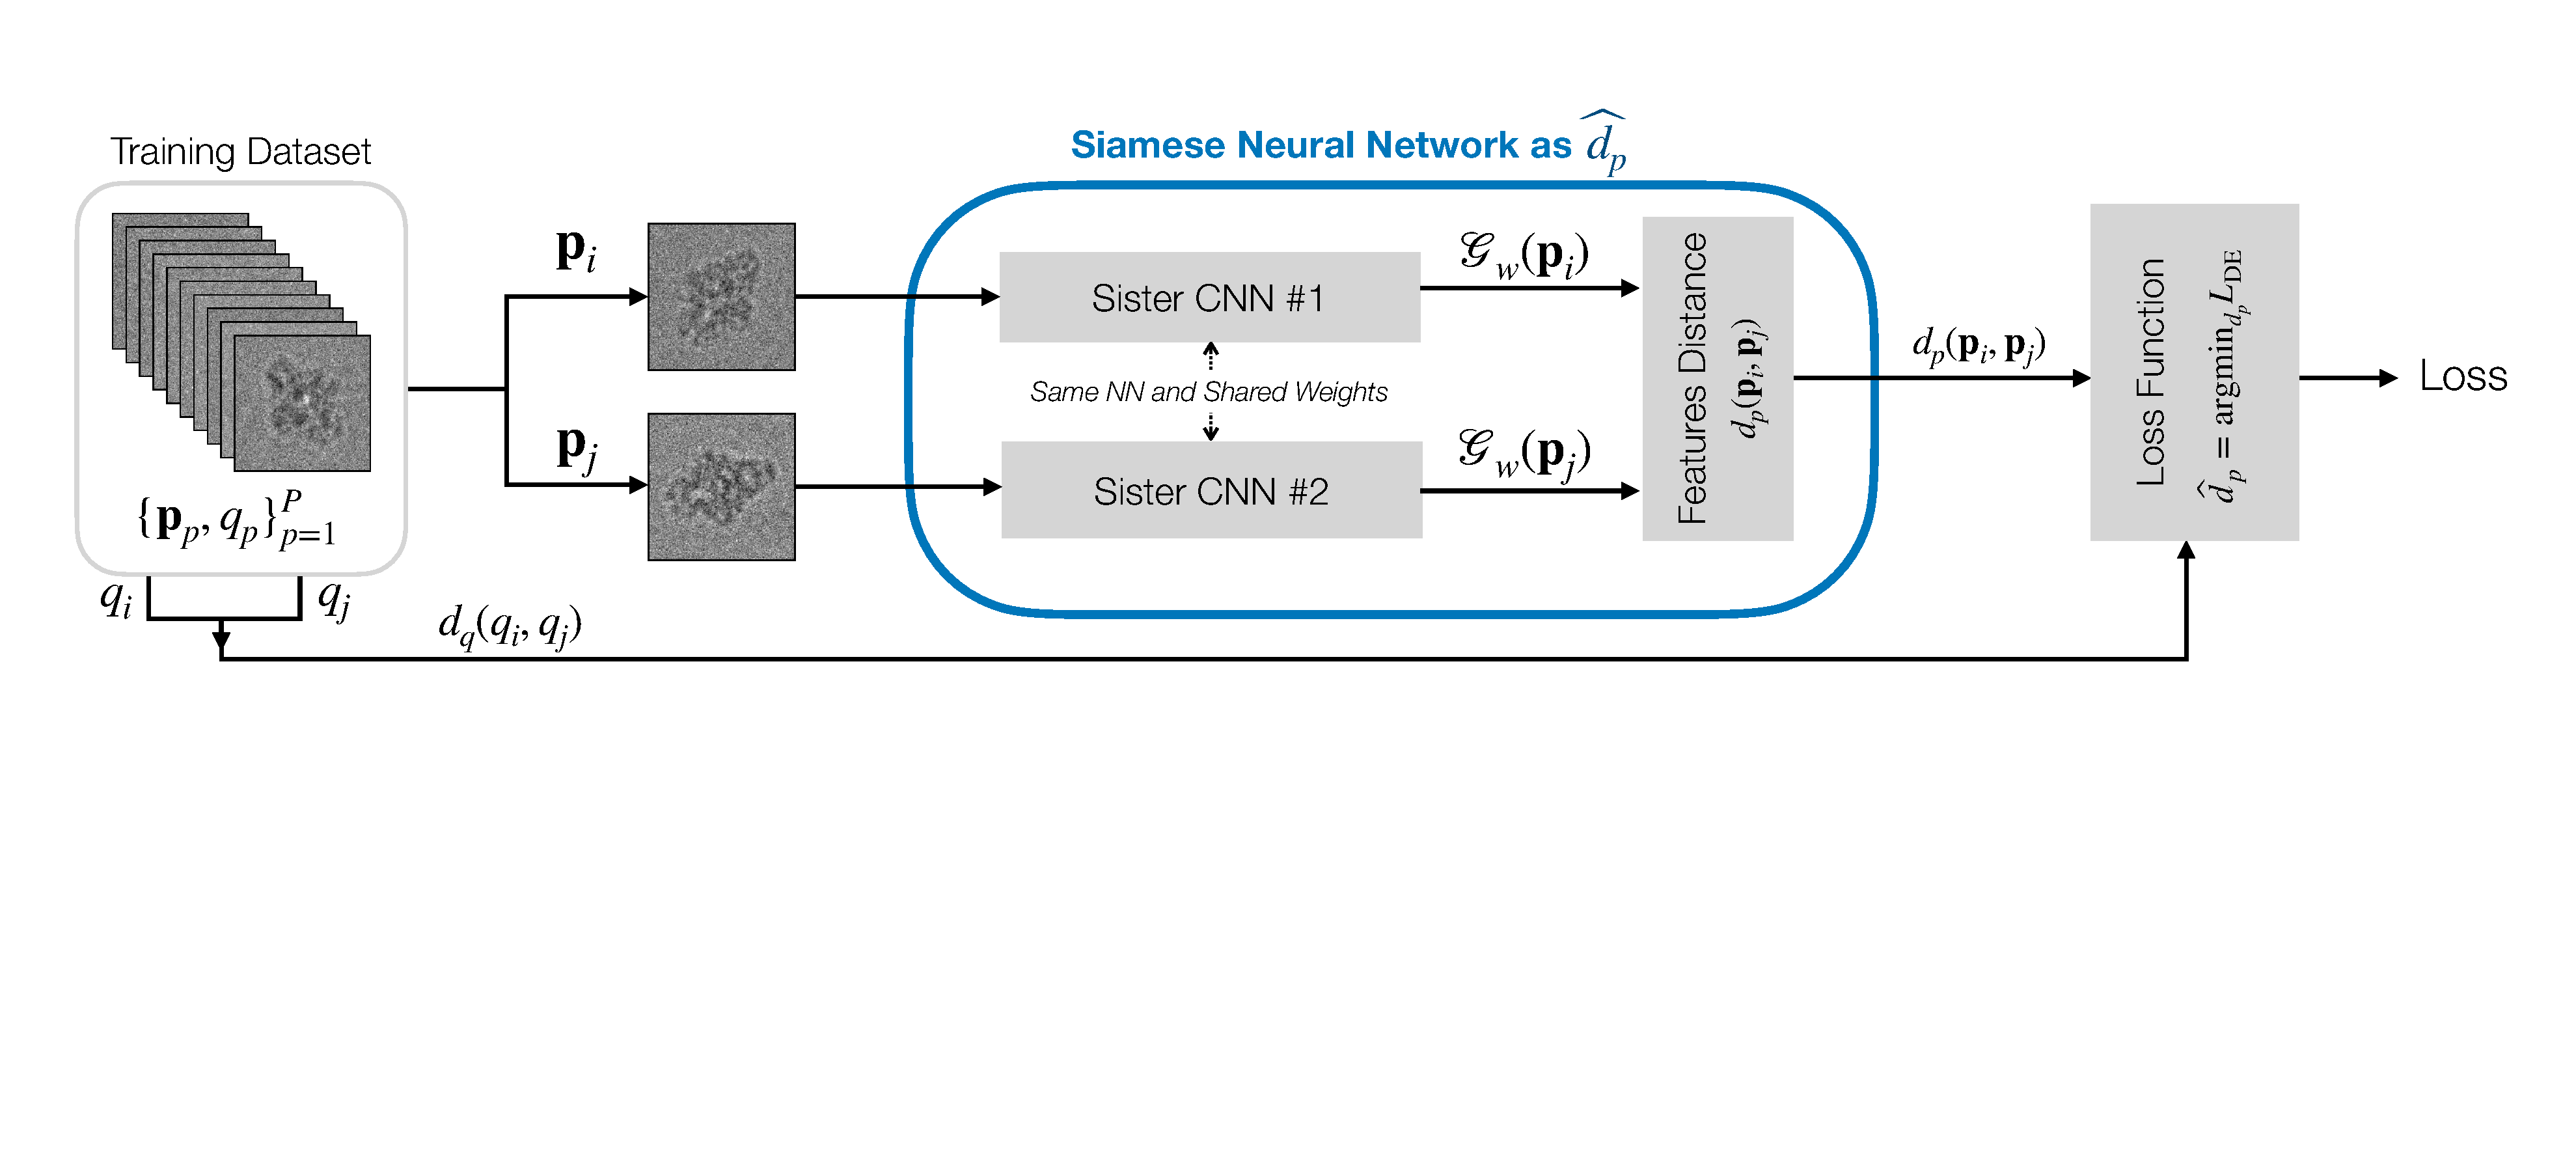
\includegraphics[width=\linewidth]{schematic_distance_learning}
    \caption{%
        \textbf{Distance learning.}
        We are looking for a distance $d_p$ between projections that is an accurate estimator of the distance $d_q$ between their orientations.
        We propose to parameterize $d_p$ as a Siamese neural network (SiameseNN), trained on a synthetic dataset of $P \approx 10^3$ \mdeff{not more?} projections with associated orientation.
        %\mdeff{Why the output "loss" arrow? To me, this system is closed.}
        %\mdeff{"Loss Function" could be called Optimization or Learning or Training.}
}\label{fig:schematic:distance-learning}
\end{figure}

From a training dataset ${\{ \mathbf{p}_{i}, q_i \}}_{i=1}^{P}$, we learn the projection distance
\begin{equation}
    \widehat{d_p} = \argmin_{d_p} \sum_{i,j} \left| d_p\big(\mathbf{p}_{i},\mathbf{p}_{j}\big) - d_q\big(q_i,q_j\big) \right|^2,
    \label{eqn:distance-learning}
\end{equation}
with $d_q$ defined in~\eqnref{distance:orientations}.
The distance $d_p$ is parameterized as the Siamese neural network (SiameseNN)~\cite{chopra2005learning}
\begin{equation*}
    d_p(\p_i, \p_j) = d_f(\G_w(\p_i), \G_w(\p_j)),
    %\label{eqn:distance:projections}
\end{equation*}
where $\G_w$ is a convolutional neural network with weights $w$ that is trained to extract the most relevant features $\f_i \in \R^{n_f}$ from a projection $\p_i$. SiameseNNs, also termed ``twin networks'', are commonly used in the field of deep metric learning to learn similarity functions~\cite{yi2014deep}.
The distance in the feature space $d_f$ is often taken to be the Euclidean distance $d_f(\f_i, \f_j) = \Vert \f_i - \f_j \Vert_2$.
To facilitate the learning of a distance that respects the elliptic geometry of $\mathbb{S}^3$, we set $d_f = d_q$.
\figref{schematic:distance-learning} illustrates the proposed learning paradigm.

As evaluating a sum over $\frac{P^2-P}{2}$ pairs is computationally intractable,
%for cryo-EM datasets with typically $P$ in the order of $10^5$ projections.
we minimize \eqnref{distance-learning} by stochastic gradient descent (SGD) over small batches of pairs and update weights by back-propagation.
% error / objective value

\subsection{Orientation recovery}\label{sec:method:orientation-recovery}
%\subsection{Orientation recovery from relative orientations}

The task of recovering points based on their relative distances has been extensively studied.
%For dimensionality reduction and data visualization, the distances are often computed from high-dimensional data.
Many methods aim at mapping high-dimensional data onto a lower-dimensional space while preserving distances, primarily for dimensionality reduction and data visualization.
%A set of distances is often built as an intermediate step.
%More specifically, these algorithms take a matrix of distances and find vectors in a lower dimensional space that accurately match the inter-vector distances.
Well-known examples include multi-dimensional scaling (MDS)~\cite{cox2008mds}, Isomap~\cite{tenenbaum2000isomap}, locally linear embedding (LLE)~\cite{roweis2000lle}, Laplacian eigenmaps~\cite{belkin2003laplacian}, t-distributed stochastic neighbor embedding (t-SNE)~\cite{maaten2008tsne}, and uniform manifold approximation and projection (UMAP)~\cite{mcinnes2018umap}.
The embedding of distance matrices in Euclidean space (given by their eigenvectors) is especially well-described.
In particular, the framework of Euclidean distance matrices (EDMs)~\cite{dokmanic2015edm} provides theoretical guarantees on the recovery of points from distances.

We however aim to embed the orientations $q$ in $\mathbb{S}^3$ (\secref{method:orientation-representation}), a setting in which we are unaware of any theoretical characterizations (e.g., on the shape of the loss function or its behavior when distances are missing or noisy).
The fact that $\mathbb{S}^3$ is locally Euclidean however offers some hope. % on the feasibility of this minimization.
Indeed, despite the non-convex loss function and the lack of theoretical guarantees, we are able to appropriately minimize our loss function, as we experimentally demonstrate in Appendix~\ref{apx:results:orientation-recovery:exact}.

We recover the orientations of a set of projections $\big\{ \mathbf{p}_k \big\}_{k=1}^P$ through
\begin{equation}
    \big\{ \widehat{q_k} \big\}_{k=1}^P = \argmin_{\{q_k \in \mathbb{S}^3\}} \sum_{i,j} \left| \widehat{d_p} \left( \p_i, \p_j \right) - d_q\left(q_i,q_j\right) \right|^2,
    \label{eqn:orientation-recovery}
\end{equation}
where $\widehat{d_p}$ is the estimator trained in \eqnref{distance-learning}.
Note that the sole difference with~\eqnref{distance-learning} is that the minimization is performed over the orientations $q$ rather than the distance $d_p$.
Here too, the sum is sampled in practice as \eqnref{orientation-recovery} is minimized by mini-batch SGD.
Sampling the sum amounts to building a sparse (instead of complete) distance graph before embedding, a common strategy.
%We experimentally demonstrate in \secref{results:orientation-recovery:exact} that neither approximation affects recovery performance.

\subsection{Evaluation}\label{sec:method:evaluation}

%\todo{Introduce the mean recovery error as a good and intuitive performance metric.}
%\todo{Figure that shows a typical convergence and mean orientation recovery error before and after alignment. We'll subsequently only report $E$ (the error after alignment).}

While not a part of the method, we get to evaluate the orientations recovered by~\eqnref{orientation-recovery}.
% (without reconstructing the protein)
%Before discussing the results, we remark that one cannot directly quantify the performance of~\eqnref{orientation-recovery} through its loss nor visual judgment of the protein reconstruction.
Unfortunately, we cannot directly take the difference between the recovered orientations $\{\widehat{q_k}\}_{k=1}^P$ and the true orientations $\{q_k\}_{k=1}^P$ as orientations are rotations up to an arbitrary reference orientation.
Any global rotation or reflection of the recovered orientations is as valid as any other, i.e., $d_q(q_i, q_j) = d_q(\T q_i , \T q_j) \; \forall \, \T \in \Or(4)$, where $\Or(4)$ is the group of $4 \times 4$ orthogonal matrices. % that represent the symmetries of $\mathbb{S}^3$ (isometries of $\R^4$) of 4D Euclidean space.
Hence, we get to best align the sets of orientations and compute the \textit{mean orientation recovery error} as
\begin{equation}
    E = \min_{\T \in \Or(4)} \frac{1}{P} \sum_{i=1}^P \big| d_q\left( q_i, \T \widehat{q_i} \right) \big|.
    \label{eqn:orientation-recovery-error}
\end{equation}
We implement $\T$ as a product of $\binom{4}{2}=6$ independent rotations and an optional reflection:
\begin{equation*}
    \T =
    \begin{bmatrix}
        m & \mathbf{0} \\
        \mathbf{0} & \mathbf{I} \\
    \end{bmatrix}
    \prod_{1 \leq i < j \leq 4} \mathbf{T}_{\theta_{ij}},
    \quad m \in \{-1,1\}, \; \theta_{ij} \in [0, 2\pi[,
\end{equation*}
where $m = \det(\T) = -1$ if $\T$ includes a reflection, and $\mathbf{T}_{\theta_{ij}} \in \SO(4)$ is a rotation by angle $\theta_{ij}$ on the $(x_i, x_j)$ plane.
%While it requires optimization, this performance metric is intuitive as it gives average error of the estimated orientations.

In practice, we again sample the sum and minimize \eqnref{orientation-recovery-error} by gradient descent with the FTRL optimizer~\cite{mcmahan2013ftrl}.
Because $\Or(4)$ is disconnected, we optimize the 6 angles separately for $m = 1$ (proper rotations) and $m = -1$ (improper rotations).
%Unless stated otherwise
We run FTRL with a learning rate of $2$, a learning rate power of $-2$, a batch size of $256$; and report the lowest of 6 runs (3 per value of $m$) of 300 steps each.

\section{Experiments}

%\lau{Move this paragraph somewhere.} 
To evaluate our method, we started with the orientation recovery experiments that included tests of feasibility and sensitivity to distance estimation error. 
We then learned the distance using a SiameseNN and compared its performance with the baseline. 
%After developing and tuning the architecture of the network for the distance estimation, we continue by introducing the perturbation to the projections.  and the network architecture is adjusted
The robustness of the network to perturbations is then evaluated.
Finally, we ran the whole machine learning pipeline to recover the orientations from estimated distances.

\subsection{Experimental conditions}\label{sec:results:data}

%\paragraph{Proteins.}
%\lau{Put pas tense everywhere.} 
We considered two proteins (\figref{pdb-proteins}): the $\beta$-galactosidase, a protein with a dihedral (D2) symmetry, and the lambda excision HJ intermediate (HJI), an asymmetric protein with local cyclic (C1) symmetry. 
Their deposited PDB atomic models are \texttt{5a1a}~\cite{bartesaghi2015betagal} and \texttt{5j0n}~\cite{laxmikanthan2016structure}, respectively.
For each atomic model, we generated the ground truth by fitting a 5\AA\ density map in Chimera~\cite{pettersen2004ucsf}, which gave us a volume of $110 \times 155 \times 199$ voxels for the $\beta$-galactosidase, and a volume of $69 \times 57 \times 75$ voxels for the HJI.

\begin{figure}[ht!]
    \centering
    \begin{subfigure}[b]{0.45\textwidth}
        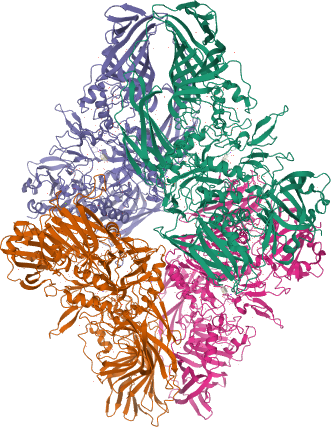
\includegraphics[height=5cm]{figures/5a1a_pdb.png}
        \caption{}
    \end{subfigure}
    %\hfill
    %\hspace{0.5em}
    \begin{subfigure}[b]{0.5\textwidth}
    \centering
        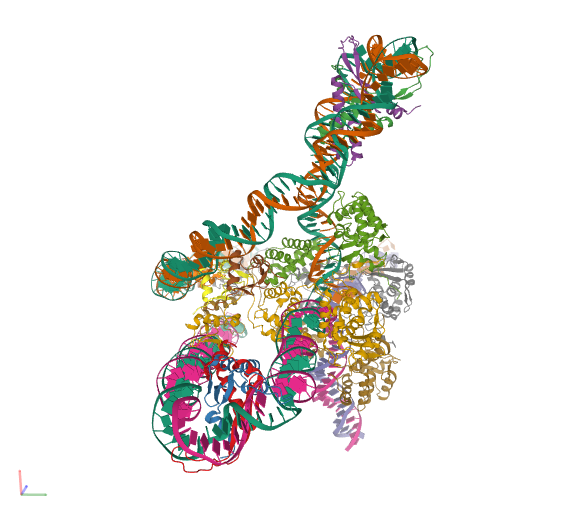
\includegraphics[height=5cm]{figures/5j0n_pdb.png}
        \caption{}
    \end{subfigure}
    \caption{%
        The two ground-truth proteins:
        \textbf{(a)} $\beta$-galactosidase (\texttt{5a1a})~\cite{5a1a_pdb}.
        \textbf{(b)} lambda excision HJ intermediate (HJI) (\texttt{5j0n})~\cite{5j0n_pdb}.
    }\label{fig:pdb-proteins}
\end{figure}


\paragraph{Projections.}
From these ground truths, we generated $5,000$ synthetic projections of size $275\times 275$ and $116\times 116$, respectively, using the ASTRA projector~\cite{van2015astra}.
Our projection generator supports two orientation samplings: (i) sampling the Euler angles $\bth=(\theta_1,\theta_2,\theta_3)$ uniformly, and (ii) sampling uniformly on $\SO(3)$.
Due to protein symmetries, orientations were sampled differently.
The entire \texttt{5j0n} complex being asymmetric~\cite{doi:10.1002/9780470514160.ch4} makes it sufficient to sample the \textit{half} of the $\mathbb{S}^2$ sphere, since the other half will have equivalent projections that are symmetric to the center of this sphere.
Conversely, the $\beta$-galactosidase has D2 symmetry, i.e., it is composed of four identical sub-units with two rotations of magnitude $\pi$ rad around the first axis followed by $\pi$ rad rotation around second axis, as illustrated and explained in~\cite{symmetry_in_protein,symmetry,scipion-em-github, rcsb-symmetry-view, EmpereurMot2019GeometricDO}.
Therefore, we restricted the sampling to the quarter of $\mathbb{S}^2$ sphere for this protein.
%\mdeff{We should explain why.}
\figref{different-projections} shows example projections.

\begin{figure}[ht!]
    \centering
    \begin{subfigure}[b]{0.24\textwidth}
        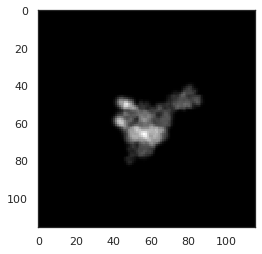
\includegraphics[height=3cm]{figures/5j0n_noise0}
        \caption{}
    \end{subfigure}
    %\hfill
    %\hspace{1.5em}%
    \begin{subfigure}[b]{0.24\textwidth}
    \centering
        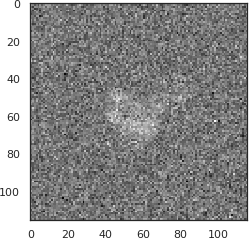
\includegraphics[height=3cm]{figures/5j0n_noise16}
        \caption{}
    \end{subfigure}
    %\hfill
    %\hspace{1.5em}%
    \begin{subfigure}[b]{0.24\textwidth}
    \centering
        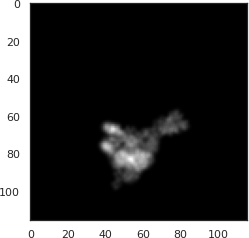
\includegraphics[height=3cm]{figures/5j0n_translated}
        \caption{}
    \end{subfigure}
    
    \caption{%
        An example of perturbed projection.
        \textbf{(a)} Unperturbed projection $\mathbf{P}_{\bth_i} \mathbf{x}$.
        \textbf{(b)} Perturbed projection $\mathbf{P}_{\bth_i} \mathbf{x} + \mathbf{n}$, with noise $\mathbf{n}$ sampled from a Gaussian distribution of mean 0 and variance 16.
        \textbf{(c)} Perturbed projection $\mathbf{S}_{\mathbf{t}} \mathbf{P}_{\bth_i} \mathbf{x}$, with translations $t_1$ and $t_2$ sampled from a triangular distribution with a lower limit of -20 pixels, an upper limit of 20 pixels, and a mode (i.e., peak) of 0.
    }\label{fig:different-projections}
\end{figure}

\paragraph{Perturbations.}
We considered the following perturbations to control the difficulty of orientation recovery: (i) additive white noise, (ii) translations, (iii) inclusion of the effects of the point-spread functions (PSF). 
The mathematical formulation of these three components is given in \eqnref{imaging-model}.

\begin{table}[ht!]
    \centering
    \begin{tabular}{lrrr}
        \toprule
        Dataset & Number of projections $P$ (\%) & Maximum number of pairs $P^2$ & Used number of pairs \\
        \midrule
        Train & 2512 (50\%) & 6,312,656 & 63,126 (1\%) \\
        Validation & 1650 (33\%) & 2,722,500 & 27,225 (1\%) \\
        Test & 838 (17\%) & 701,406 & all (sampled per batch) \\
        \bottomrule
    \end{tabular}
    \caption{
        Split of $P=5000$ projections (for both \texttt{5j0n} and \texttt{5a1a}) in training, validation, and test sets.
    }\label{tab:dataset}
\end{table}

\paragraph{Distance learning.}
We used the supervised learning where the input are pairs of images and the output is their respective quaternion distance calculated from the ground truth orientations.
For the training, dataset was split into a distinct training, validation, and testing set (see \tabref{dataset}).
The total number of generated projections was $P = 5,000$.
Therefore, the number of possible projection pairs was $P^2 = 25e6$.
Splitting $P^2$ into the training, validation, and testing sets would mean that some of the projections appearing in pairs in the training dataset can appear in pairs in the other datasets.
To ensure that the results generalize to unseen data, we split the projections $P$ (and not $P^2$) into training, validation, and testing projection sets.
With these three projections sets we create disjoint projection pair datasets sets (column with $P^2$ values in \tabref{dataset}).
In addition to this, we use only $1\%$ of the possible pairs (last column in the \tabref{dataset}) due to limitation of available resources for the training.
%\todo{Better explain why projections (and not pairs) must be separated in the various sets.}


\paragraph{Orientation recovery.}
Orientations were recovered through \eqnref{orientation-recovery} in a stochastic setting, with the loss function varying over the batches.
To ensure unbiased model, the dataset used in this part was test set from \tabref{dataset}.
Orientation recovery was performed on projections unseen during distance learning.
Since mean orientation error is used in the pose estimation tasks and it is considered reliable performance metric, we decided to use it as our performance measure (see Appendix~\ref{apx:metrics-review}). The average difference between predicted and actual angles is degree (or rad), which makes it an intuitive comparison metric. 
We employ the definition of a correct estimation: the estimation must be within 10\degree~(0.174 rad) of true orientations for noiseless data and within 25\degree~(0.436 rad) for noisy data.
\figref{5j0n-aa-loss-perfect-distances} shows a successful convergence and mean orientation recovery error before and after alignment with the perfect distance $d_q$.


%\mdeff{Why is it good? Intuitive sure. Laurène, can we say something more?}

%%%%%%%%%%%%%%%%%%%%%%%%%%%%%%%%%%%%%%%%%%%%%%%%%%%%%%%%%%%%%%%%%%%%%%%%%%%%%%%%%%%%%%%
%\subsection{Results}\label{sec:results:orientation-recovery}



%\mdeff{Story: good distance estimation = good orientation recovery.}
% \begin{algorithm}[H]
% \SetAlgoLined
% \KwResult{Write here the result }
%  initialization\;
%  \For{$steps \gets 1$ \textbf{to} $30000$}{
%   instructions\;
%   \eIf{condition}{
%   instructions1\;
%   instructions2\;
%   }{
%   instructions3\;
%   }
%  }
%  \caption{Orientation recovery algorithm}
% \end{algorithm}


%\subsubsection{Robustness of Recovery to Additive Errors on the Relative Distances}

%%%%%%%%%%%%%%%%%%%%%%%%%%%%%%%%%%%%%%%%%%%%%%%%%%%%%%%%%%%%%%%%%%%%%%%%%%%%%%%%%%%%%%%

\subsection{Sensitivity of orientation recovery to errors in distance estimation}\label{sec:results:orientation-recovery:sensitivity}

%\mdeff{Story: (i) orientation recovery error is strongly linked to distance estimation error, (ii) recovery loss is a good proxy of mean recovery error.}

To prove that orientation recovery is feasible, we first evaluate the performance assuming we have ideal distance metric between two projections, i.e., the quaternion distance between their corresponding orientations. 
The method successfully recovers the orientation of every projection, see Appendix~\ref{apx:results:orientation-recovery:exact}.

We now go one step further and evaluate the behaviour of~\eqnref{orientation-recovery} when the true relative distances are corrupted by additive Gaussian noise.
The experimental conditions are the same as in the previous section, except that we add an error with increasing variance on the relative distances prior to the minimization. Precisely: $d_p = d_q + n$ with $n$ sampled from a Gaussian distribution with mean 0 and variances in $[0.0, 0.8]$.
The results are presented in \figref{perfect-with-noise-ar-aa} (red curve).
For all variances, the mean orientation recovery error $E$ is reported in \figref{perfect-with-noise-ar-aa} (blue curve).

\begin{figure}[ht!]
    \centering
    \begin{subfigure}[b]{0.48\textwidth}
        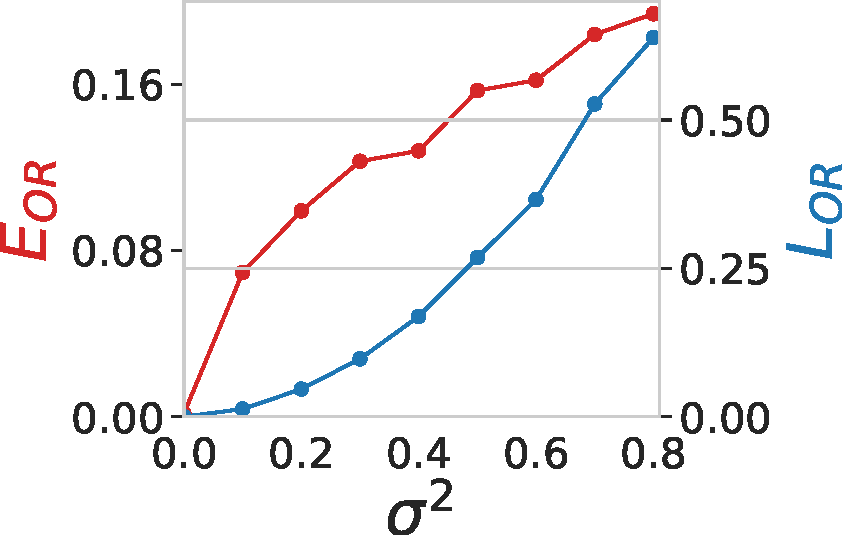
\includegraphics[height=5cm]{figures/5j0n_perfect_noisy_ar_aa}
        \caption{Asymmetric protein (\texttt{5j0n}).}
    \end{subfigure}
    \hfill
    \begin{subfigure}[b]{0.50\textwidth}
    \centering
        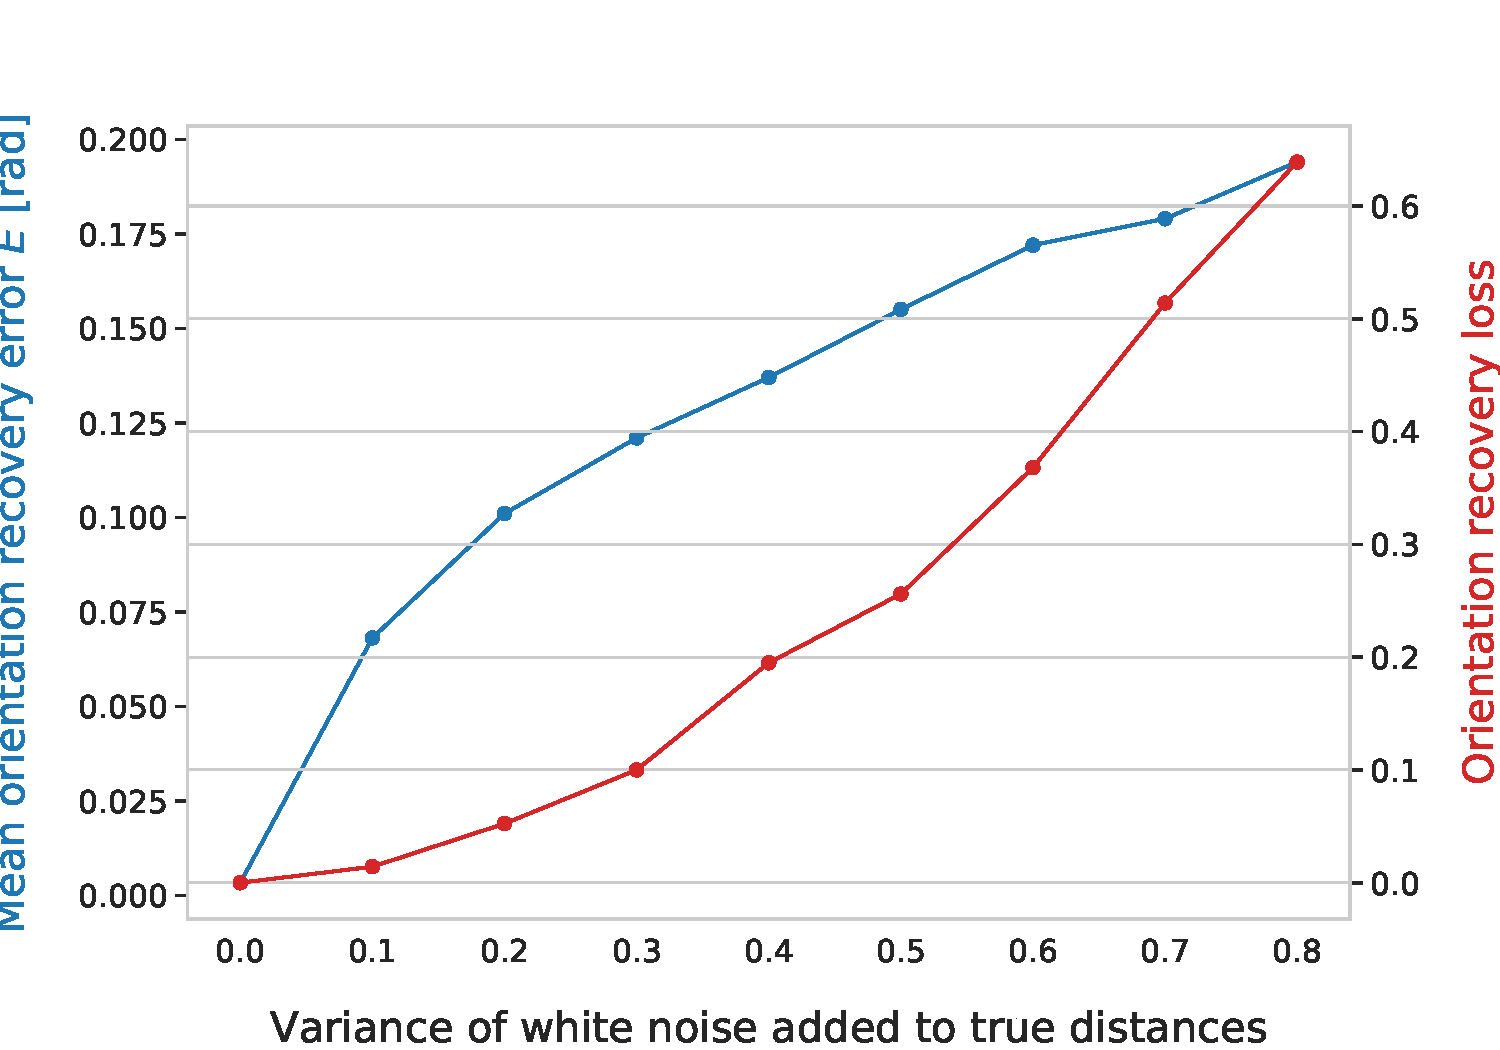
\includegraphics[height=5cm]{figures/5a1a_perfect_noisy_ar_aa}
        \caption{Symmetric protein (\texttt{5a1a}).}
    \end{subfigure}
    \caption{
        The mean orientation recovery error $E$ from \eqnref{orientation-recovery-error} is a monotonic function of the distance estimation error.
        Better distance estimation leads to better orientation recovery.
        Moreover, the recovery loss \eqnref{orientation-recovery} is a good proxy for the recovery error $E$, allowing us to assess recovery performance even without ground-truth orientations.
}
    \label{fig:perfect-with-noise-ar-aa}
\end{figure}

These results demonstrate that the performance of orientation recovery~\eqnref{orientation-recovery} depends on the quality of the estimated distances, which advocates for a proper and extensive training of the SiameseNN in the next stages of development.
Another interesting output of \figref{perfect-with-noise-ar-aa} is that it indicates that the error of the orientation recovery behaves as a monotonic function of its loss.
Hence, it suggests that the loss can be used as a good indicator of its performance, which has obvious practical implications for our future works on real data.

%%%%%%%%%%%%%%%%%%%%%%%%%%%%%%%%%%%%%%%%%%%%%%%%%%%%%%%%%%%%%%%%%%%%%%%%%%%%%%%%%%%%%%%

\subsection{Learned function for relative distance estimation }\label{sec:results:distance-estimation:learned}

%\mdeff{Story: learned distance $d_{ps}$ estimates $d_q$ with some variance but still underestimates larger distances.
%Again symmetric vs asymmetric.}

We present here a preliminary evaluation of the ability of SiameseNNs to learn a projection distance $\widehat{d_p}$ that correctly approximates the orientation distance $d_q$. 
To assess the progress and effectiveness of our distance estimation implementation, we used an Euclidean distance as a baseline (see Appendix~\ref{apx:results:distance-estimation}).

%SiameseNNs come with a variety of more or less powerful architectures.
%At the current stage of development, we work with a simple one.
%Our SiameseNN is composed of two convolutional neural networks (CNNs) with shared weights.
%Their output features vectors are compared through an Eulidean distance, \textit{i.e.}, $d_f(\mathbf{f}_i,\mathbf{f}_j)=\lVert \mathbf{f}_i-\mathbf{f_j}\rVert_2$ in \figref{schematic:distance-learning}.
%Besides the Euclidean distance, this distance metric $F$ can be defined as geodesic distance, or it could be parametrized as MLP, used for a general function approximation, which we will explore in some of the following experiments.
%\mdeff{Don't repeat what's written in \secref{method:distance-learning}. The general stuff goes there, the specific here.}

\begin{figure}
    \centering
    \begin{subfigure}[t]{0.45\textwidth}
        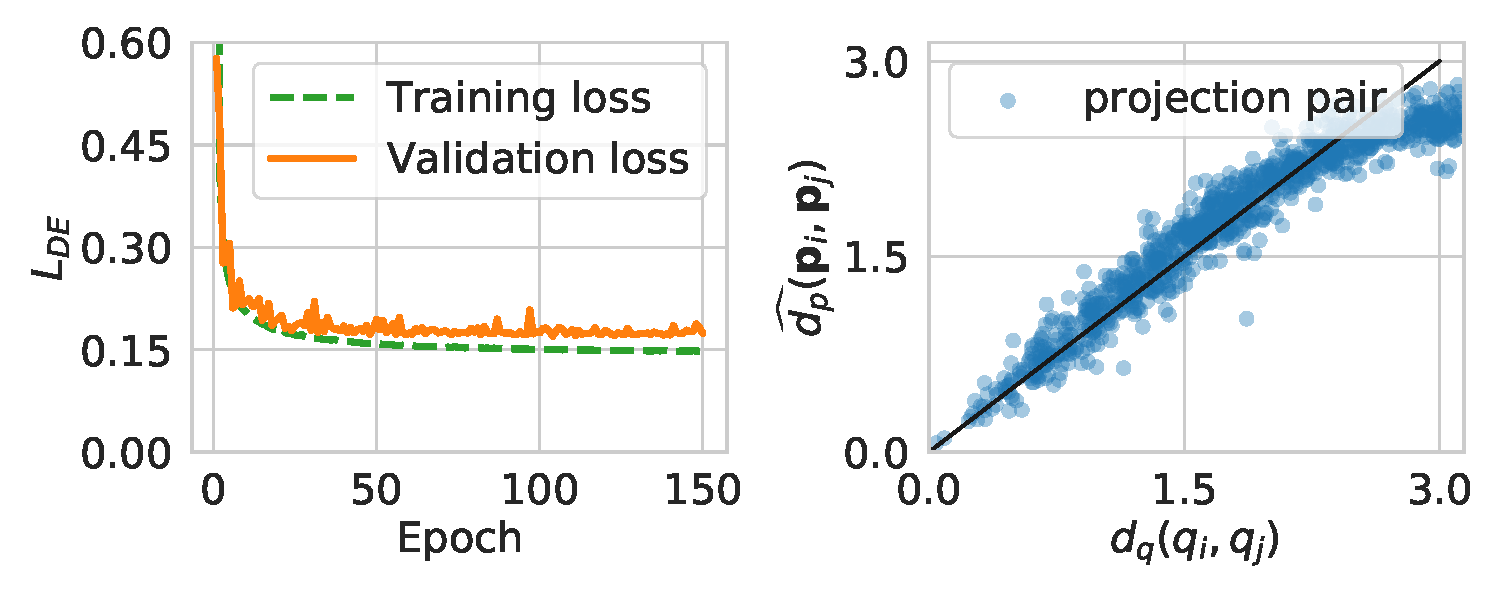
\includegraphics[height=3.5cm]{figures/de_loss_dPdQ_5j0n.pdf}
        \caption{Asymmetric protein (\texttt{5j0n}).}
        \label{fig:losses-siamese-assym}
    \end{subfigure} \quad \quad
    \begin{subfigure}[t]{0.5\textwidth}
        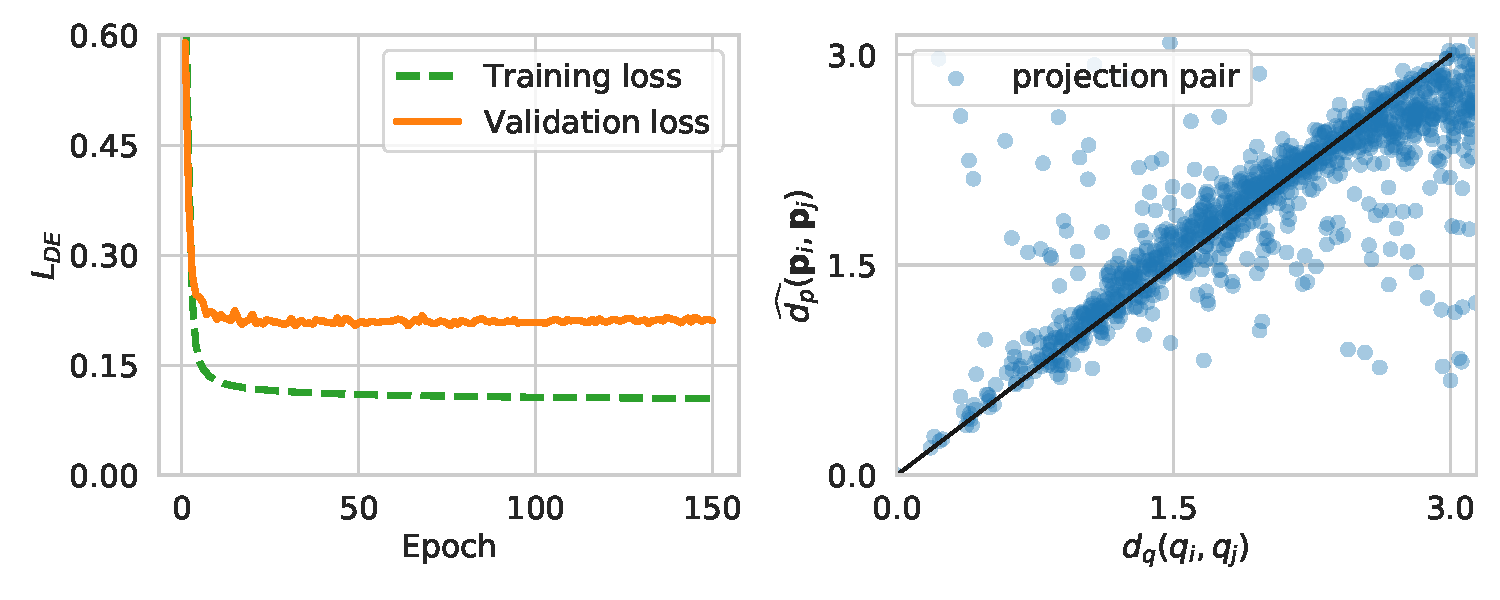
\includegraphics[height=3.5cm]{figures/de_loss_dPdQ_5a1a.pdf}
        \caption{Symmetric protein (\texttt{5a1a}).}
        \label{fig:losses-siamese-sym}
    \end{subfigure}
    \caption{
        Distance learning loss \eqnref{distance-learning} evaluated on the training and validation datasets during learning/training (on the left side respectively). Relationship between orientations' distance $d_q$ and estimated distance $d_p$ on the test dataset (on the right side respectively).
    }\label{fig:losses-siamese}
\end{figure}

% \begin{figure}
%     \centering
%     \begin{subfigure}[b]{0.5\columnwidth}
%         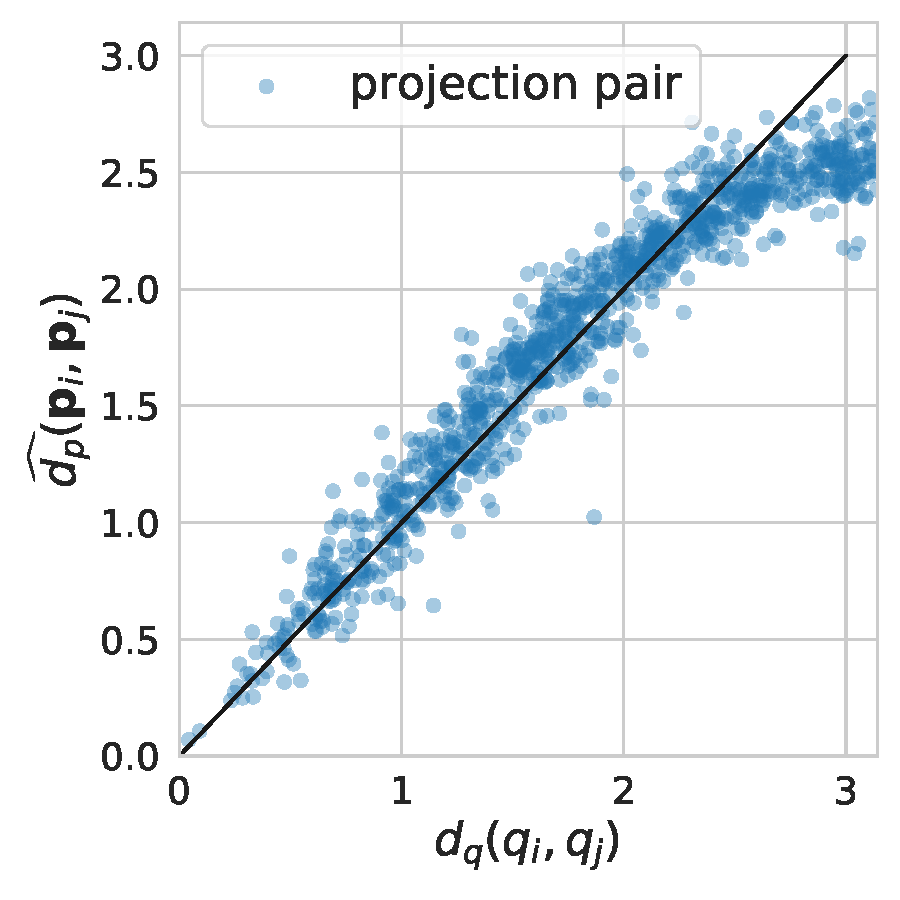
\includegraphics[height=6cm]{figures/dPdQ_5j0n}
%         \caption{Asymmetric protein (\texttt{5j0n}) on test dataset.}
%     \end{subfigure}
%     %\hfill
%     \begin{subfigure}[b]{0.45\columnwidth}
%     \centering
%         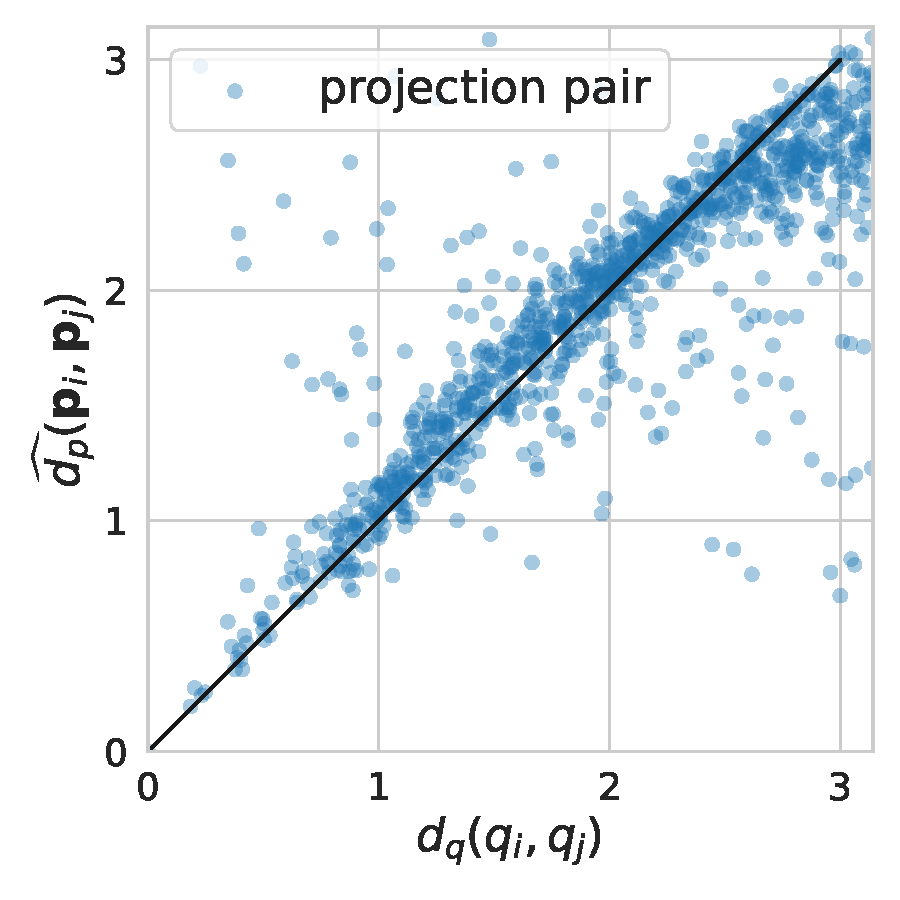
\includegraphics[height=6cm]{figures/dPdQ_5a1a}
%         \caption{Symmetric protein (\texttt{5a1a}) on test dataset.}
%     \end{subfigure}
%     \caption{Relationship between orientations' distance $d_q$ and estimated distance $d_p$.}
%     \label{fig:learned-distance-siamese}
% \end{figure}

%\mdeff{What is $d_f$ in this particular experiment? Euclidean? Cosine=$d_q$?}
For each protein, we trained the SiameseNN on its training dataset for 150 epochs ($\sim$2.6 hours) using an RMSProp optimizer~\cite{tieleman2012rmsprop}, a learning rate of $10^{-3}$, and a batch size of 256 pairs. 
As a feature distance $d_f$ between the outputs of the two CNNs we used the Geodesic distance \eqnref{geodesic-distance}.
The pairs for the training were sampled from $1\%$ of maximum number of training pairs $P_{\text{train}}^2$ ($63,126$ pairs) and validation was performed on $1\%$ of the maximum number of validation pairs $P_{\text{val}}^2$ ($27,225$ pairs). 
We limited our training and validation dataset due to Google Colaboratory~\footnote{A hosted Jupyter notebook service from Google Research with resources that are not guaranteed and not unlimited.} training time limit of 12 hours.

%\mdeff{So those pairs are sampled from $63,126$ pairs from the training dataset, rather than the $P^2$ possible pairs? If true, we should motivate somewhere why we limit our training dataset.}
Depending on the available resources on the Google Colaboratory, the training lasted from 2.6 hours to 9.3 hours on one of its GPUs.
The evolution of the training and validation losses are presented on the left side in \figref{losses-siamese-assym} for the asymmetric protein (\texttt{5j0n}), and on the left side in \figref{losses-siamese-sym} for the symmetric one (\texttt{5a1a}).
The results demonstrate that the SiameseNN succeeded at learning a proxy distance for the asymmetric protein dataset, as convergence was reached in about 50 epochs ($\sim$ 50 minutes in the best resource availability setting).

%\todo{Mention the plateau phenomenon, similarly to Euclidean $d_p$.}
Similarly to Euclidean distance $d_p$, we noticed that the larger distances $d_q$ were poorly predicted and the plot again had a slight plateau phenomenon for the distances higher than ~$2.5$ rad.

It is interesting to see that both validation losses were around $0.2$.
However, the current SiameseNN architecture slightly overfits at learning the distance for the dataset \texttt{5a1a}, which is very likely due to the symmetry of the $\beta$-galactosidase protein, even thought the quarter-sphere coverage was used.
%Indeed, its synthetic dataset may still contain pairs of projections that share the same $d_p$, yet differ in their $d_q$.
This simply advocates for the restriction to non-overlapping areas on $\SO(3)$ when sampling the orientations used to generate the SiameseNN training dataset.
The latter would then only contain projection pairs with a linear $(d_q,d_p)$ relationship, which should ensure a successful training of the network.
%\mdeff{I don't get this explanation. Do you mean that \texttt{5a1a} might have other symmetries than D2?}
For the rest of the experiments, we used the asymmetric protein (\texttt{5j0n}) dataset.
Besides using the asymmetric protein, we performed the full protein reconstruction pipeline on the symmetric protein (\texttt{5a1a}).

We then fed to the trained SiameseNN $1,000$ pairs of projections randomly selected from the \texttt{5j0n} testing dataset, and reported the $(d_q,\widehat{d_p})$ relationship of each pair in \figref{losses-siamese} (right side of each subfigure).
These results confirm that, the SiameseNN was able to predict the orientation distance $d_q$ using only the projections as inputs. 
The prediction performance was slightly better for the asymmetric protein compared to symmetric protein.
Moreover, it clearly outperformed the Euclidean distance at doing so.
These preliminary results are encouraging, as much has yet to be gained from improving upon the rather primitive SiameseNN architecture we currently use. 
The architecture of implemented SiameseNN can be seen in Appendix~\ref{sec:siamese-architecture}. 
Besides concentrating on the hyperparameter selection and tuning of the neural network layers, we also evaluated the performance of the model depending on the feature distance we used for the SiameseNN, see\figref{geo-eucl-mlp} and Appendix~\ref{apx:de-influence-arch}.

%%%%%%%%%%%%%%%%%%%%%%%%%%%%%%%%%%%%%%%%%%%%%%%%%%%%%%%%%%%%%%%%%%%%%%%%%%%%%%%%%%%%%%%

\subsection{Sensitivity of learned distance to perturbations in the projections}\label{sec:results:distance-estimation:sensitivity}

%\mdeff{Story: learned distance is minimally sensible to perturbations (additive noise, translation, PSF) because we can train it to ignore irrelevant information.
%Thanks again to good model of cryo-EM imaging.}
%\mdeff{Better word? (perturbations, quality, non-ideal)}

In this experiment we wanted to explore how does the perturbation of the projections affect the distance estimation (additive noise, translation, PSF). 
The experimental conditions for the experiment were the same as before, except that we added noise with increasing variance on the projection prior to training.
The results are presented in \figref{distance-estimation-vary-projection-noise}.

We observe that the training and validation losses were increasing and network started to overfit w.r.t.\ the amount of noise in the projections.
With the noiseless projections (projection noise variance 0), the mean orientation recovery error $E = 0.1594$ rad.
Whereas, the noisy projections with noise levels 15 were the closest to the realistic protein projections and the error $E=0.4189$ rad.
The SiameseNN was able to learn the noise as the training loss and corresponding mean orientation recovery error $E$ stayed low.
%\mdeff{The SiameseNN seems to be able to learn the noise, as the training loss stays low. More data should help!}

Besides testing the performance of the pipeline with the noisy projections, we explored the performance with different projection translation levels.
To translate the projection, we used a triangular distribution from $-t$ to $t$ px translation with the peak in the center of the projection.
The performance of different translation magnitudes can be seen in \figref{distance-estimation-vary-projection-translation}.
We observe that the training of the network was invariant to translations in the projections, which was expected.
We can see that the learned distance was minimally sensible to perturbations because we trained the network to ignore irrelevant information.
%\mdeff{Perfect!}


\begin{figure}[ht!]
    \centering
    \begin{subfigure}[b]{0.47\textwidth}
        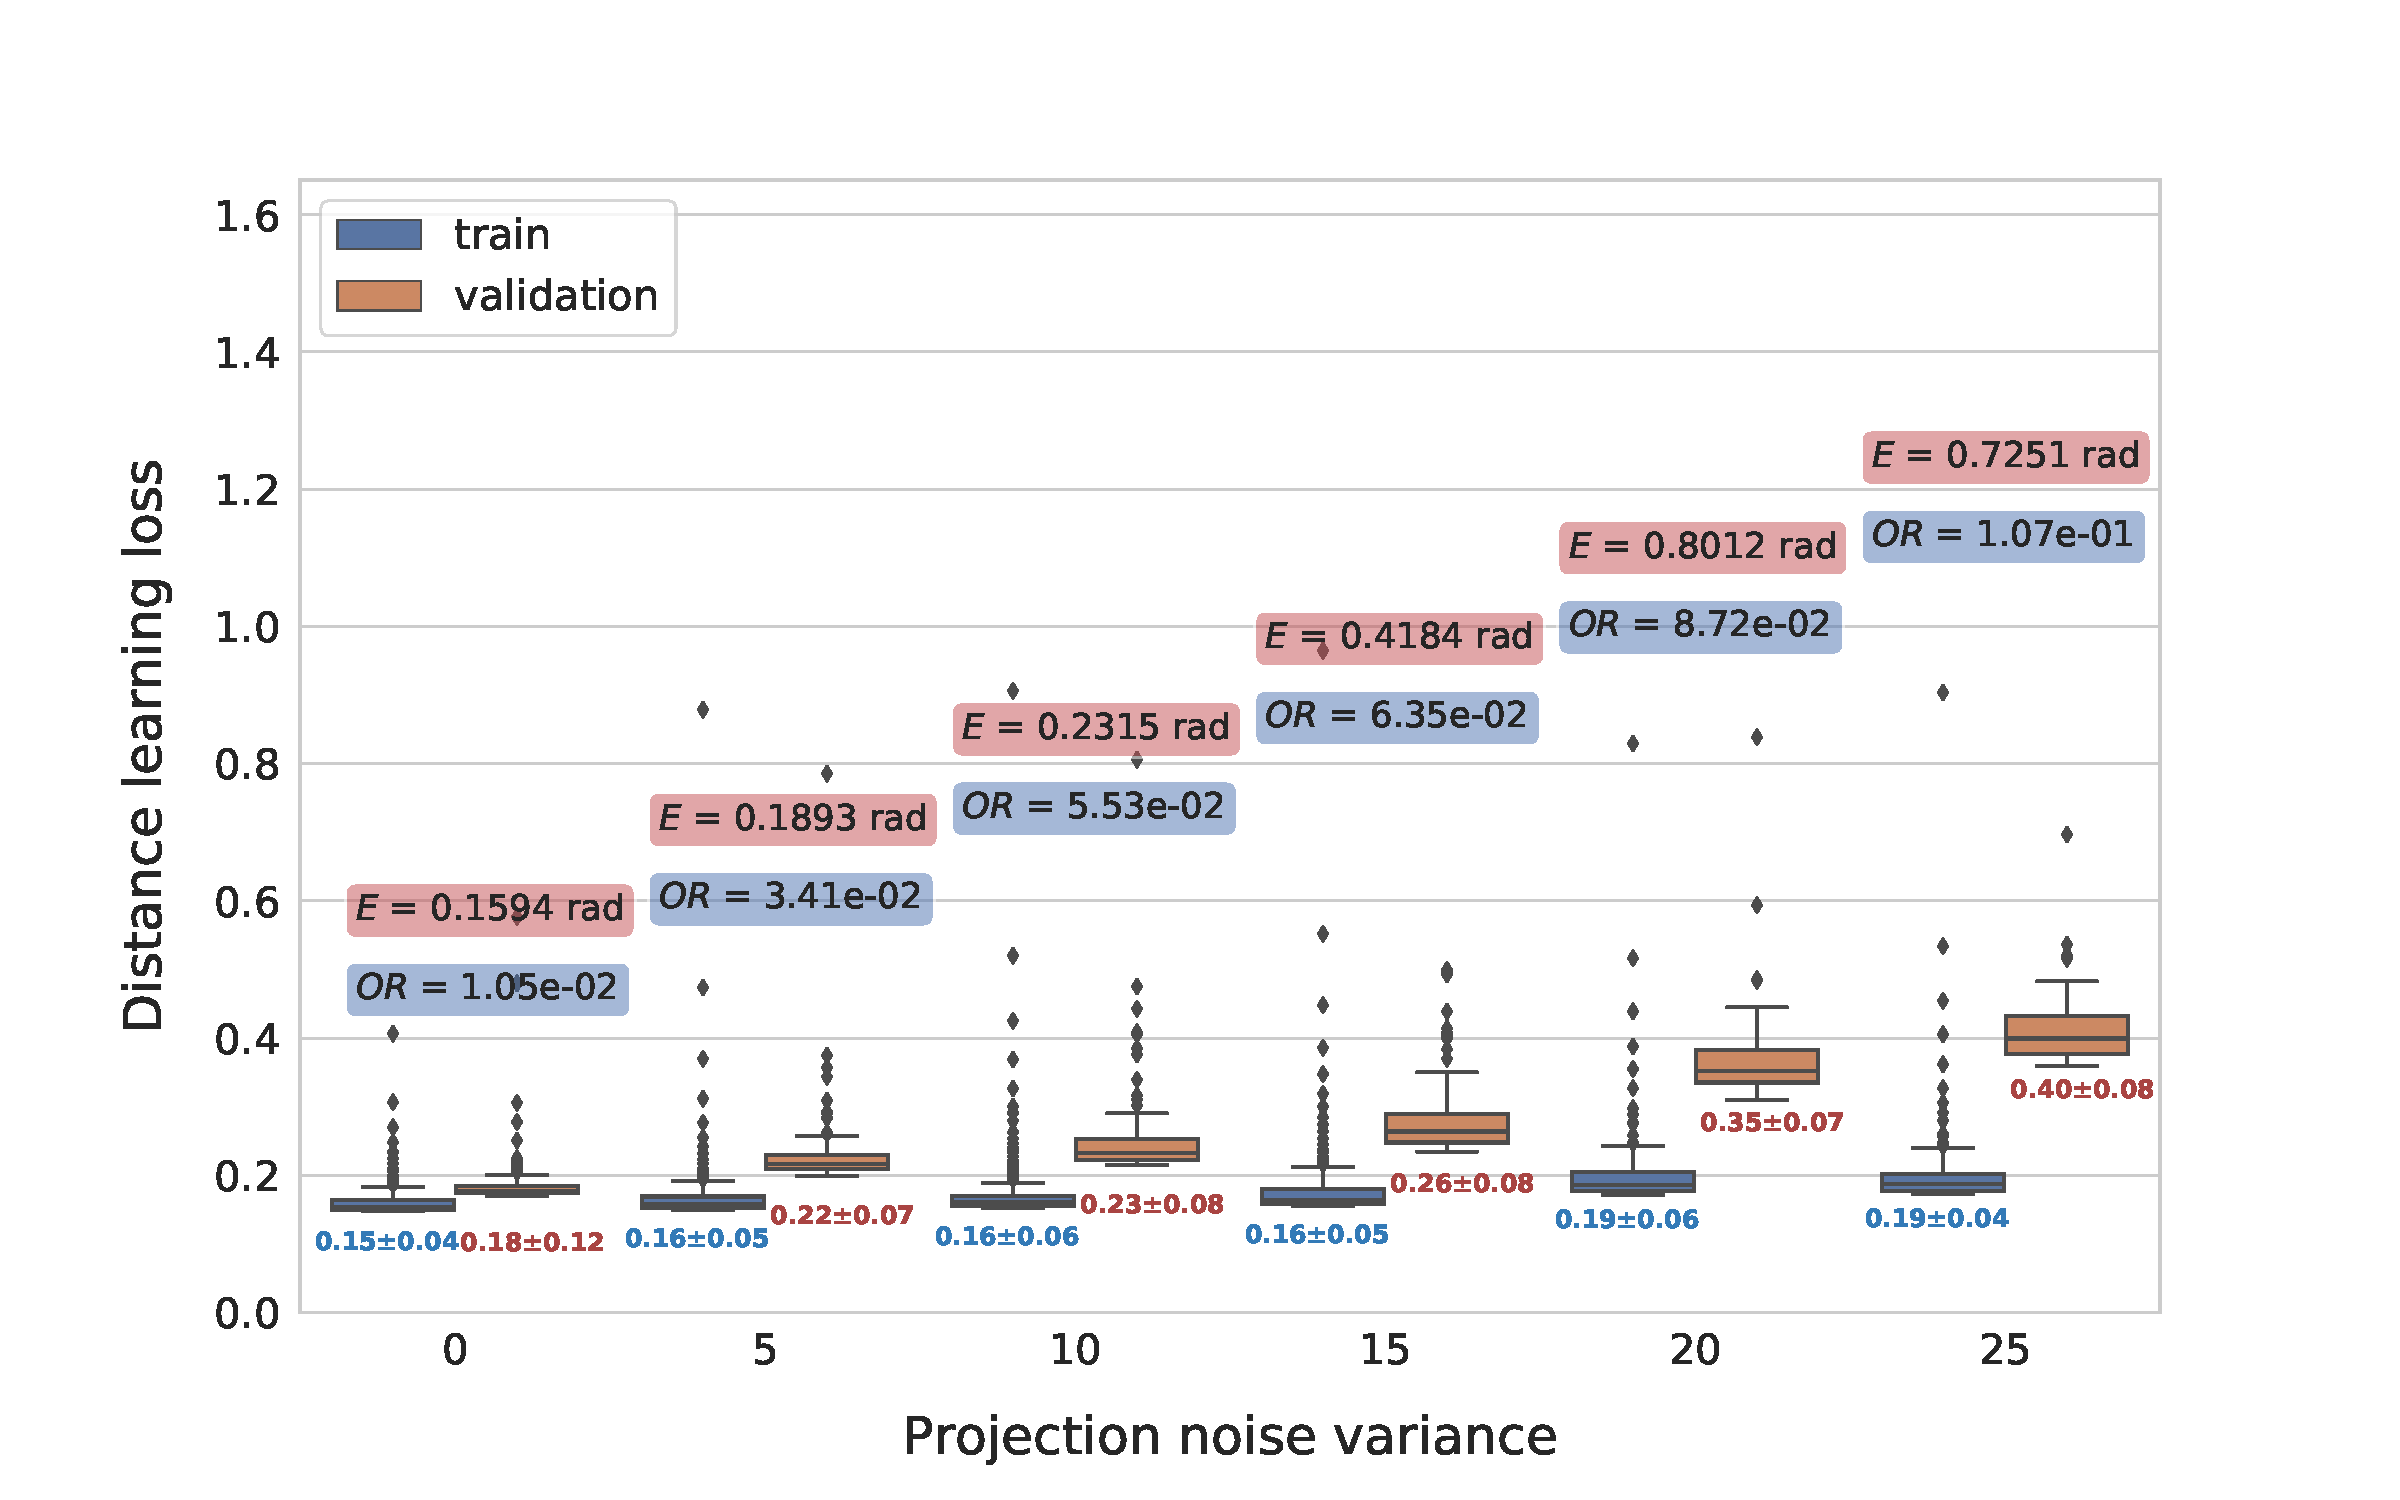
\includegraphics[height=5.5cm,valign=t]{figures/de_noises_nums}
        \caption{%
            Variation of train and validation epoch losses w.r.t. noise levels in the projections of the asymmetric protein (\texttt{5j0n}). The mean orientation recovery error $E$ is in the red box, and the orientation recovery loss $OR$ is in the blue box.
        }\label{fig:distance-estimation-vary-projection-noise}
    \end{subfigure}
    \hfill
    \begin{subfigure}[b]{0.47\textwidth}
        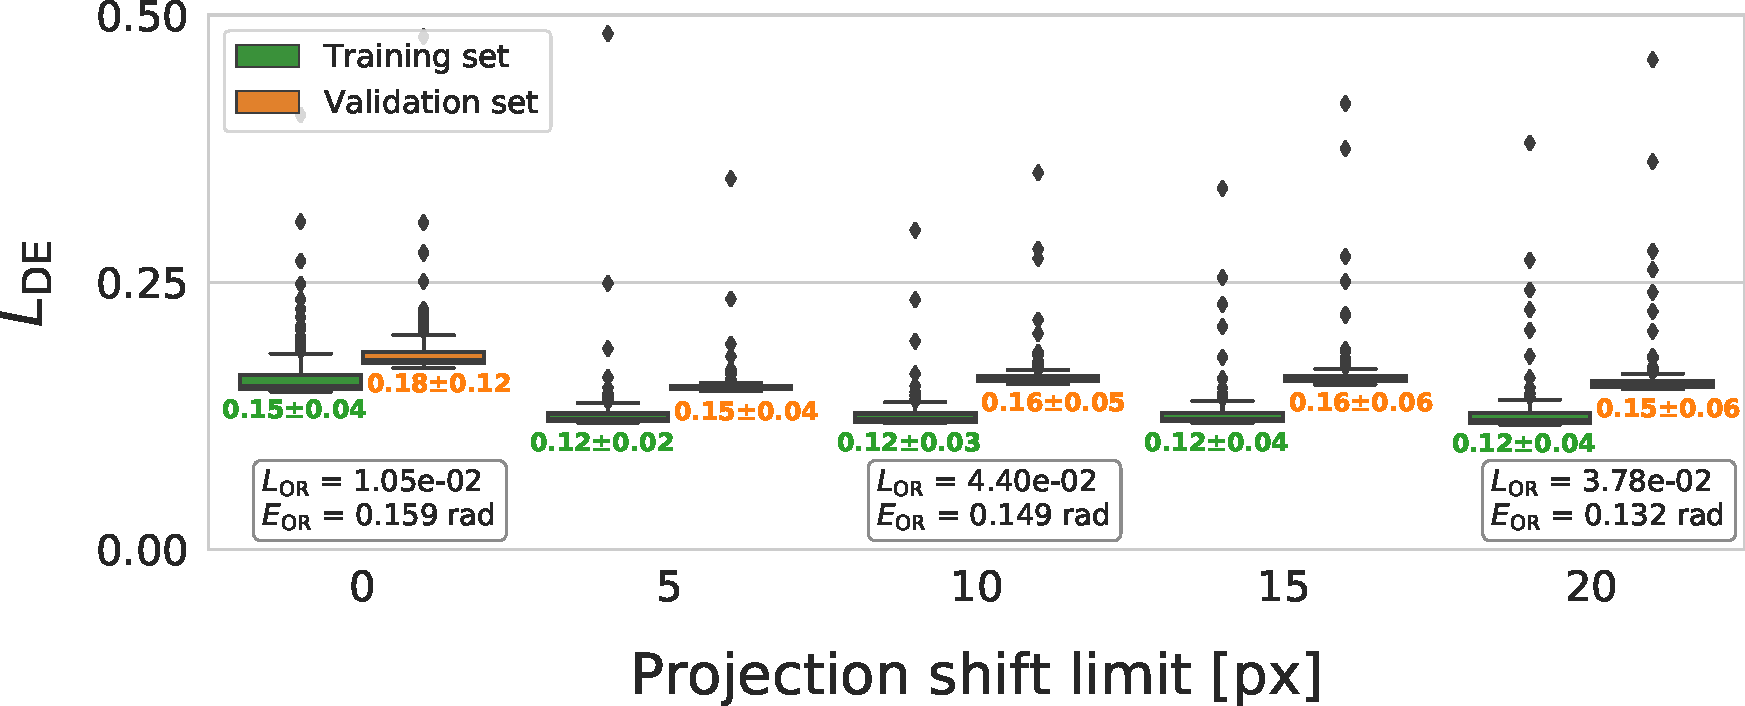
\includegraphics[height=5.5cm,valign=t]{figures/de_translation_nums}
        \caption{
        Variation of train and validation epoch losses w.r.t.\ projection translation of the asymmetric protein (\texttt{5j0n}). The mean orientation recovery error $E$ is in the red box, and the orientation recovery loss $OR$ is in the blue box.
        %\mdeff{We should try to have 12 and 13 side-by-side (to gain some space and facilitate comparison on the y-axis) by making them more square.}
    }\label{fig:distance-estimation-vary-projection-translation}
    \end{subfigure}
\end{figure}

%%%%%%%%%%%%%%%%%%%%%%%%%%%%%%%%%%%%%%%%%%%%%%%%%%%%%%%%%%%%%%%%%%%%%%%%%%%%%%%%%%%%%%%

\subsection{Orientation recovery from estimated distances}

%\mdeff{Story: pipeline works but better distance estimation is needed for SOTA reconstruction.
%Method is however promising because learned distance is robust to perturbations and recovery works if distance works.}
%\todo{Justify threshold because of plateau (figref).
%Show recovered orientations w.r.t.\ ground truth after alignment.}
%\todo{Reconstruct the protein to show the full pipeline: from a set of projections to a reconstructed protein.
%Emphasize that it's a naive reconstruction algorithm.}

The orientation recovery from estimated distances represents a full pipeline needed to reconstruct the protein from a given set of projections.
We ran the pipeline for both, asymmetric (\texttt{5j0n}) and symmetric (\texttt{5a1a}) protein.
In addition, we ran the pipeline for the simulated realistic noise in the asymmetric protein.
The experimental setting for distance estimation was similar to the one used to generate the \figref{learned-distance-siamese}: 150 epochs, 1e-3 learning rate, batch size 256 with random sampling of the projections, but for feature distance metric we used the geodesic distance since it showed the best performance in \figref{geo-eucl-mlp}.

We then ran the orientation recovery on the estimated distances of the asymmetric protein and the performance results can be observed in \figref{5j0n-orientation-recovery-loss-est} with the same experimental setting as in \figref{5j0n-orientation-recovery-loss}.
With the noiseless projections, the objective function successfully converged to the $0.0510$ and with the noisy projections, the objective function converged to the $0.0683$.

\begin{figure}[ht!]
    \centering
    \begin{subfigure}[b]{0.45\textwidth}
        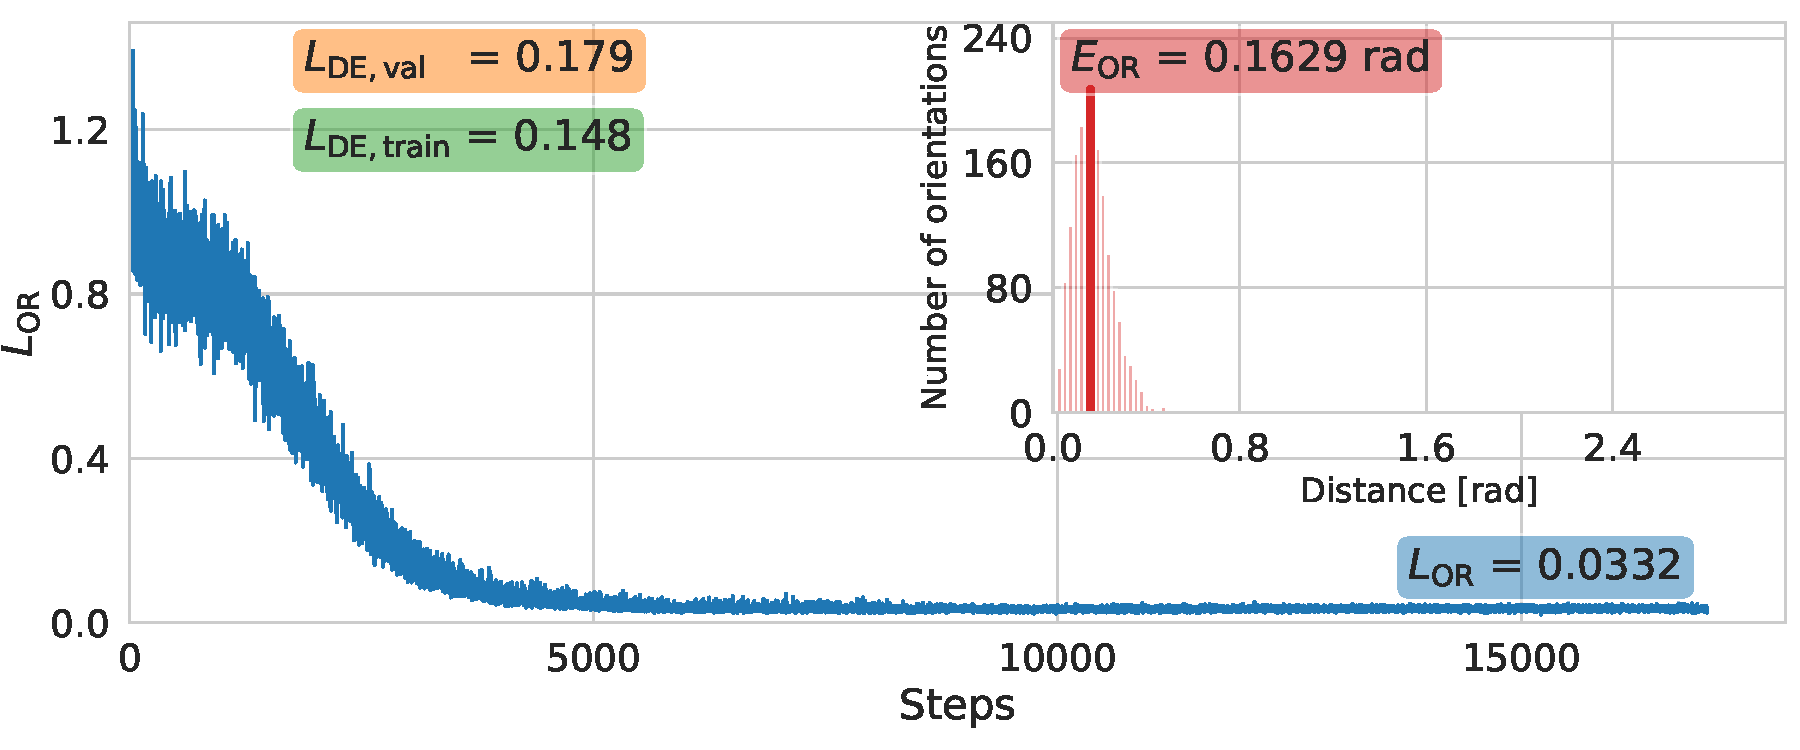
\includegraphics[height=5.5cm]{figures/5j0n_noise0_ar_aa}
        \caption{Recovery loss~\eqnref{orientation-recovery} and error~\eqnref{orientation-recovery-error} with noiseless projections $\mathbf{Px}$.}
    \end{subfigure}
    \hfill
    \begin{subfigure}[b]{0.5\textwidth}
    \centering
        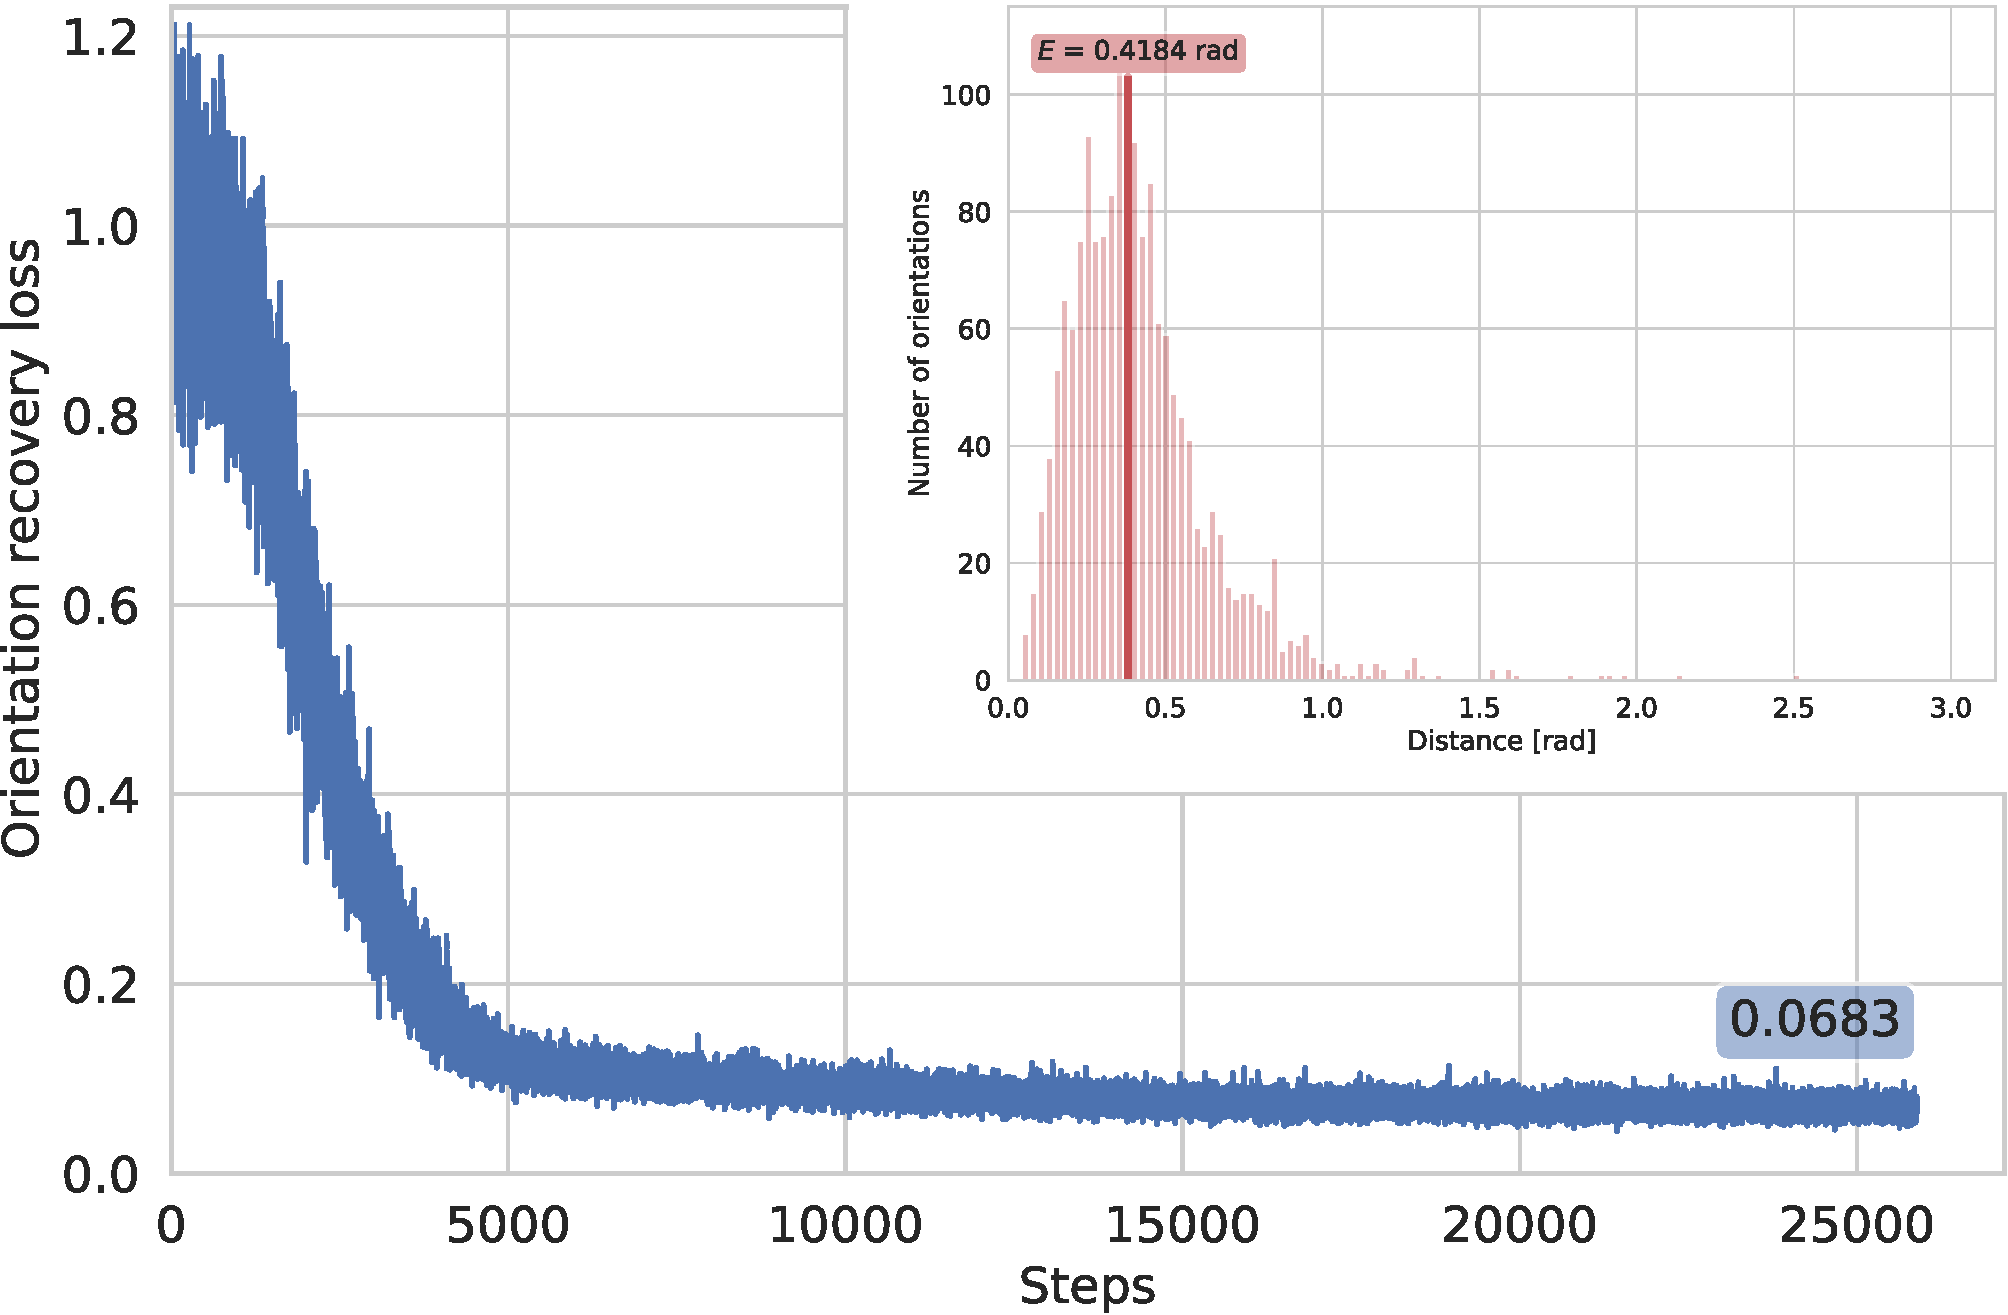
\includegraphics[height=5.5cm]{figures/5j0n_noise16_ar_aa}
        \caption{Recovery loss and recovery error with noisy projections $\mathbf{Px+n}, \; \mathbf{n} \sim \mathcal{N}(0, 16\mathbf{I})$.}
    \end{subfigure}
    \\
    % \begin{subfigure}[b]{0.45\textwidth}
    % \centering
    %     %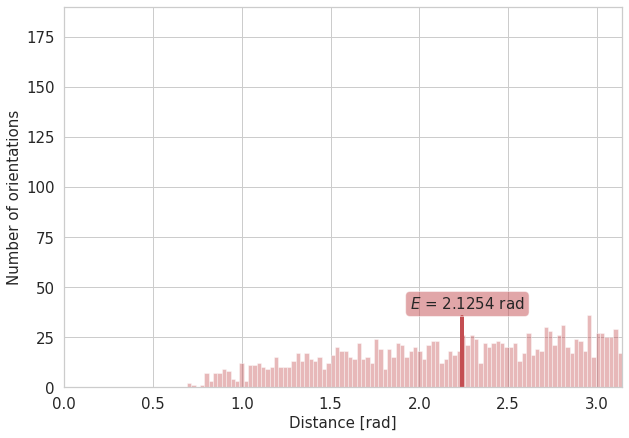
\includegraphics[height=5.7cm]{figures/5j0n_noise0_angle_alignment_before}
    %     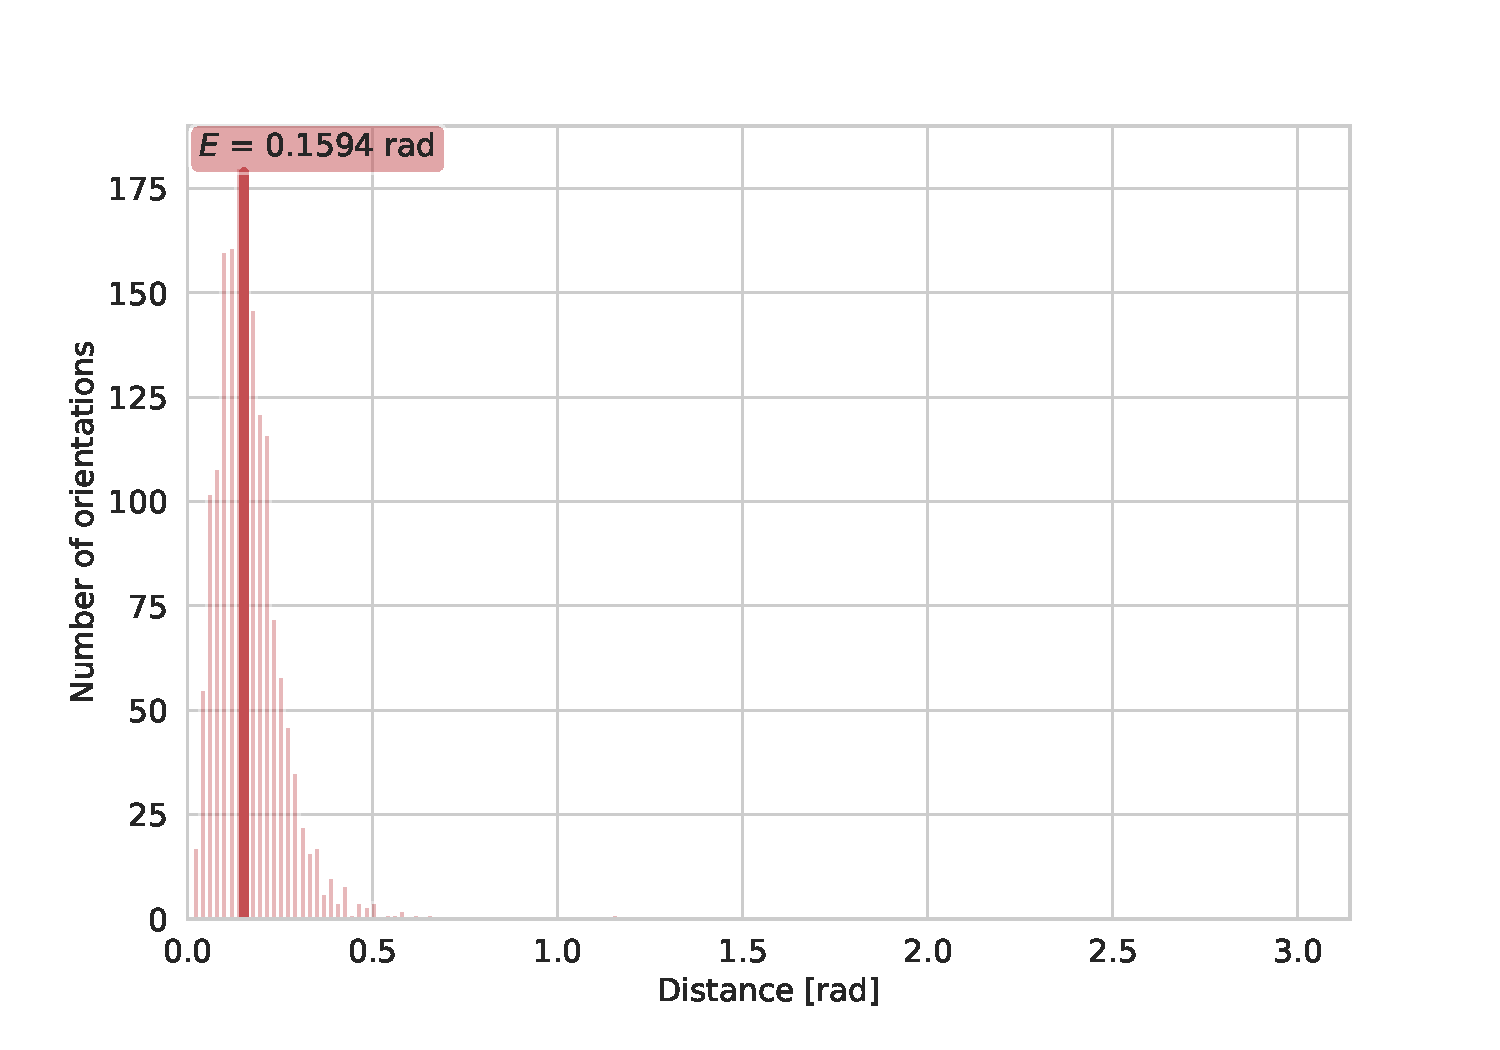
\includegraphics[height=5.7cm]{figures/5j0n_noise0_angle_alignment_after}
    %     \caption{Recovery error, noiseless projections $\mathbf{Px}$.}
    %     \label{fig:angle-alignment-5j0n-noise0}
    % \end{subfigure}
    % \hfill
    % \begin{subfigure}[b]{0.5\textwidth}
    % \centering
    %     %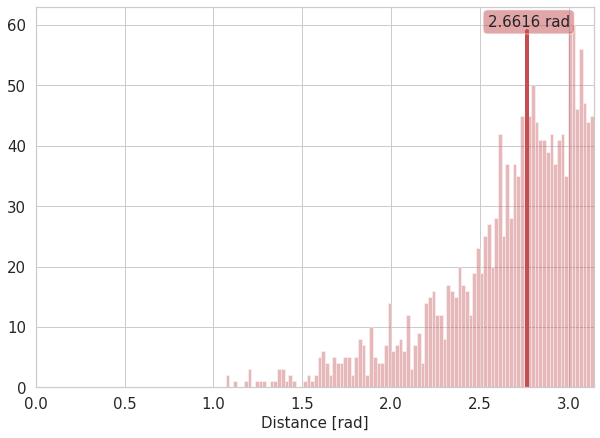
\includegraphics[height=5.7cm]{figures/5j0n_noise16_angle_alignment_before}
    %     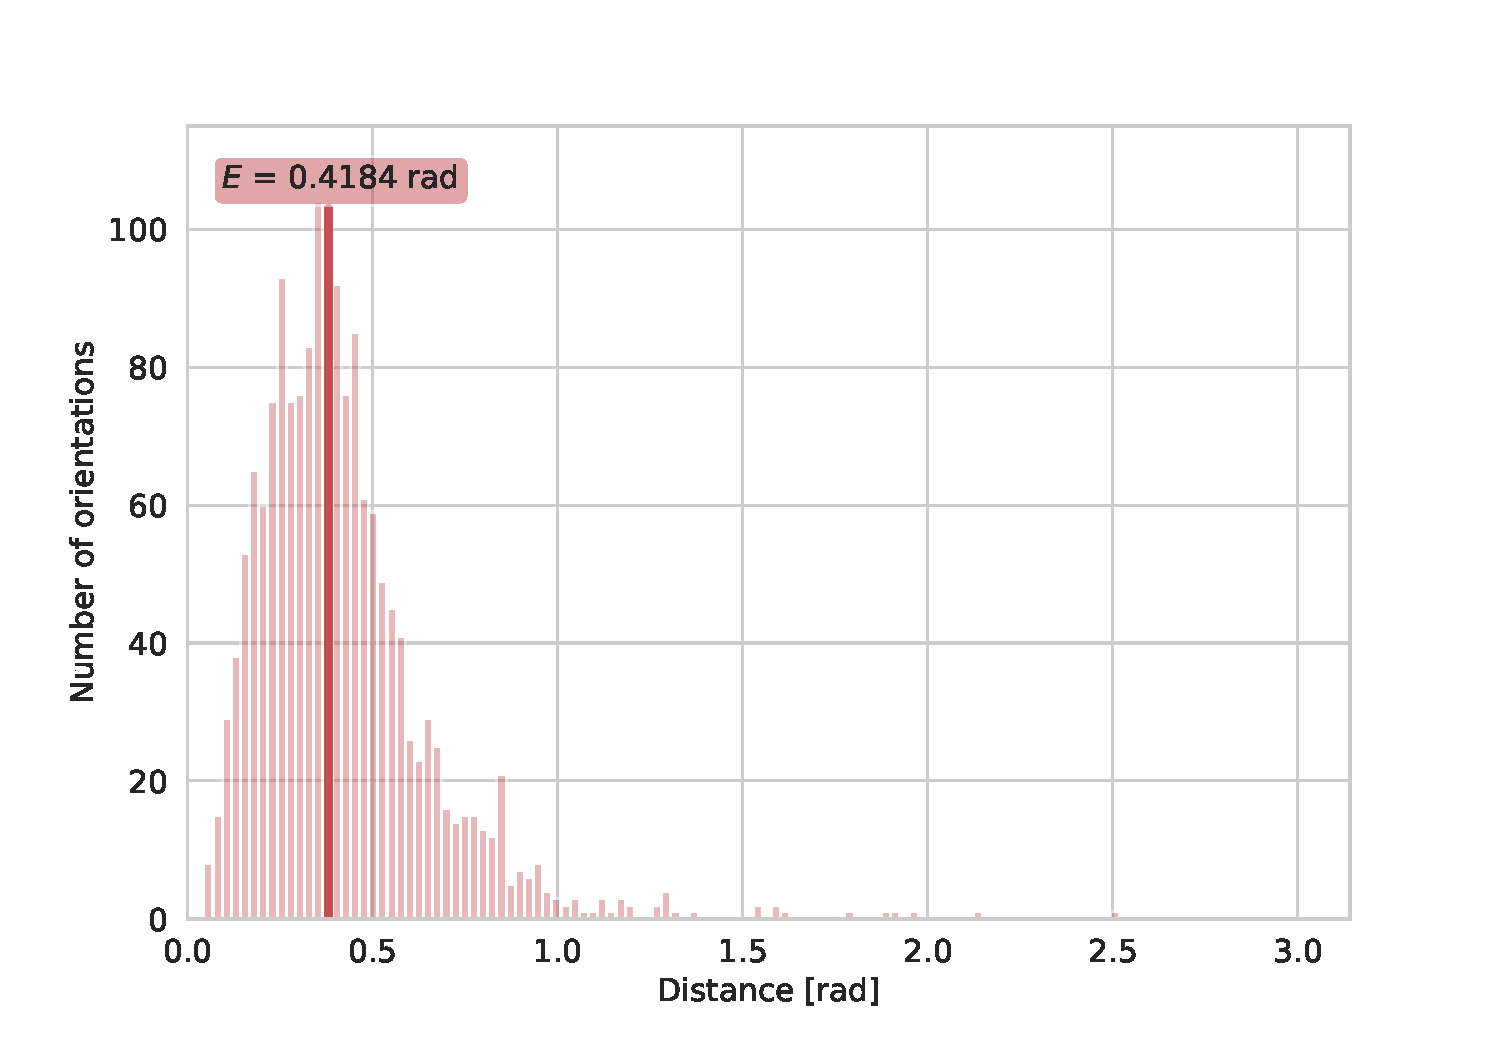
\includegraphics[height=5.7cm]{figures/5j0n_noise16_angle_alignment_after}
    %     \caption{Recovery error, noisy projections $\mathbf{Px+n}, \; \mathbf{n} \sim \mathcal{N}(0, 16\mathbf{I})$.}
    %     \label{fig:angle-alignment-5j0n-noise16}
    % \end{subfigure}
    \caption{%
        Performance of orientation recovery of the asymmetric protein (\texttt{5j0n}) with (right) and without (left) noise.
        The first row shows the orientation recovery loss.
        The second row shows the orientation recovery error ($E$ from \eqnref{orientation-recovery-error}).
    }\label{fig:5j0n-orientation-recovery-loss-est}
\end{figure}

The mean orientation recovery error for asymmetric protein \texttt{5j0n} without noise in the projection is shown in \figref{angle-alignment-5j0n-noise0}.
The smallest error achieved is $0.1594$ rad.
The mean orientation recovery error for asymmetric protein \texttt{5j0n} with noisy projections (white noise with variance 16) is shown in \figref{angle-alignment-5j0n-noise16}.
The smallest error achieved is $0.4184$ rad.

As a last step of the pipeline, we performed protein reconstruction using the projections and their corresponding estimated orientations.
Using the ASTRA toolbox, we generated orientation vectors based on angles which we fed into projection 3D geometry in ASTRA.
With total of $1,650$ projections in the test dataset, we were able to reconstruct the protein. 
The reconstruction results for the asymmetric protein (\texttt{5j0n}) with \textit{noiseless projections} are shown in \figref{5j0n-reconstruction}: \textbf{(a)} using the ground-truth orientations and \textbf{(c)} using the estimated aligned orientations. 
The reconstruction results for the asymmetric protein (\texttt{5j0n}) with \textit{noisy projections} are shown in \figref{5j0n-reconstruction}: \textbf{(b)} using the ground-truth orientations and \textbf{(d)} using the estimated aligned orientations.

\begin{figure}[ht!]
    \centering
    \begin{subfigure}[b]{0.22\linewidth}
        \centering
        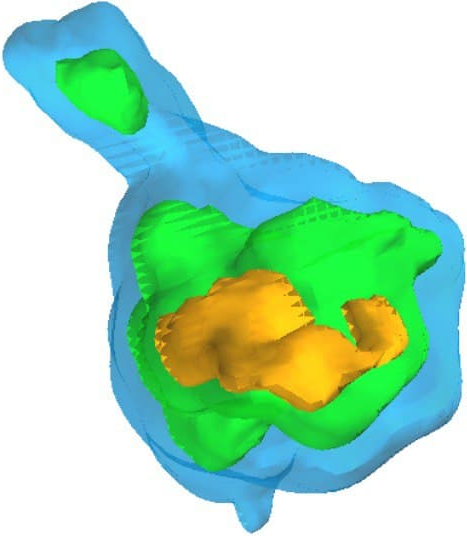
\includegraphics[width=0.99\linewidth]{figures/5j0n_reconstruction_GT}
        \caption{}
    \end{subfigure}
    \hfill
    \begin{subfigure}[b]{0.22\linewidth}
        \centering
        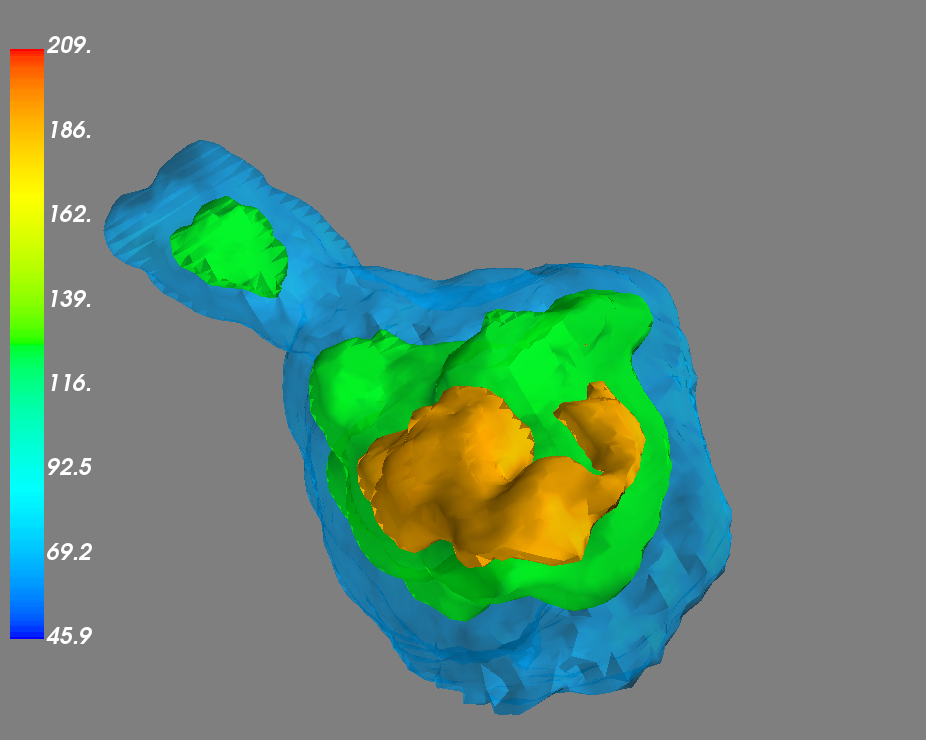
\includegraphics[width=0.99\linewidth]{figures/5j0n_reconstruction_GT_noise16}
        \caption{}
    \end{subfigure}
    \hfill
    \begin{subfigure}[b]{0.22\linewidth}
        \centering
        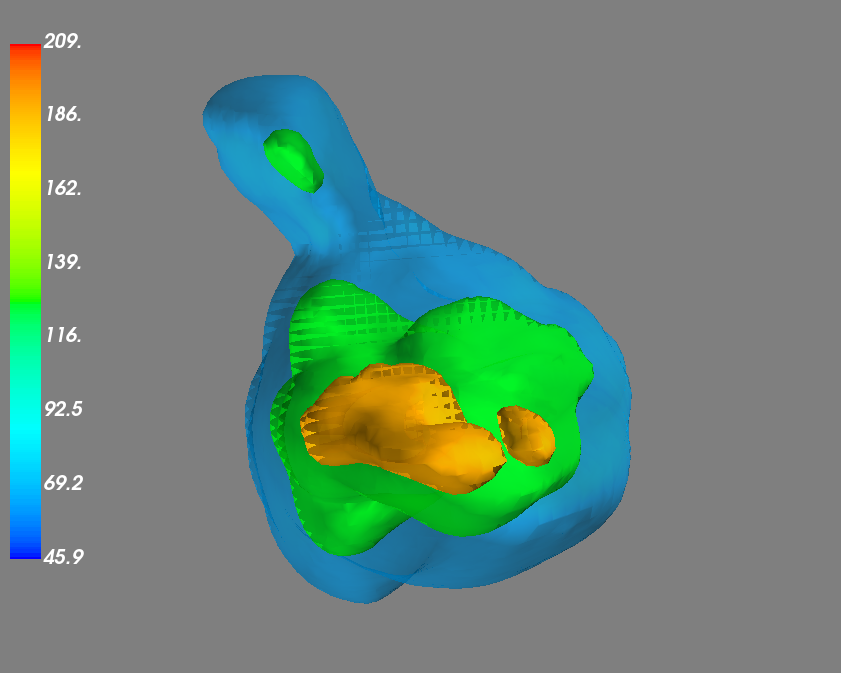
\includegraphics[width=0.99\linewidth]{figures/5j0n_reconstruction_noise0}
        \caption{}
    \end{subfigure}
    \hfill
    \begin{subfigure}[b]{0.22\linewidth}
        \centering
        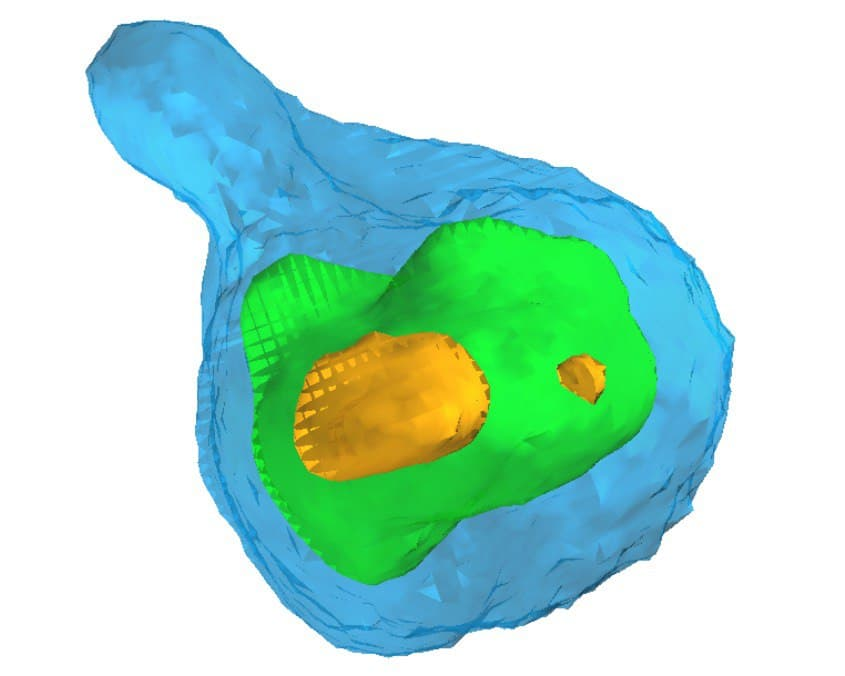
\includegraphics[width=0.99\linewidth]{figures/5j0n_reconstruction_noise16}
        \caption{}
    \end{subfigure}
    \caption{
        Performance of orientation recovery of the asymmetric protein (\texttt{5j0n}). \textbf{(a)} Noiseless projections $\mathbf{Px}$, true orientations ${\big\{q_p\big\}}_{p=1}^P$. \textbf{(b)} Noisy projections $\mathbf{Px + n}$, true orientations ${\big\{q_p\big\}}_{p=1}^P$. \textbf{(c)} Noiseless projections $\mathbf{Px}$, recovered orientations ${\big\{\widehat{q_p}\big\}}_{p=1}^P$. \textbf{(d)} Noisy projections $\mathbf{Px + n}$, recovered orientations ${\big\{\widehat{q_p}\big\}}_{p=1}^P$.
    }\label{fig:5j0n-reconstruction}
\end{figure}

Similarly, we ran the whole reconstruction pipeline on the symmetric protein (\texttt{5a1a}).
The experimental conditions for the distance estimation were the same as for the asymmetric protein, except that we used the quarter-sphere projections coverage (whereas, in the asymmetric protein we used half-sphere coverage).
The orientation recovery loss is shown in \figref{5a1a-orientation-recovery-loss}. 
It successfully converged to $0.0381$.
The mean orientation recovery error for symmetric protein \texttt{5a1a} is shown in \figref{angle-alignment-5a1a-noise0}. 
The smallest error achieved was $0.1871$ rad.

\begin{figure}[ht!]
    \centering
    \begin{subfigure}[b]{0.45\textwidth}
        \centering
        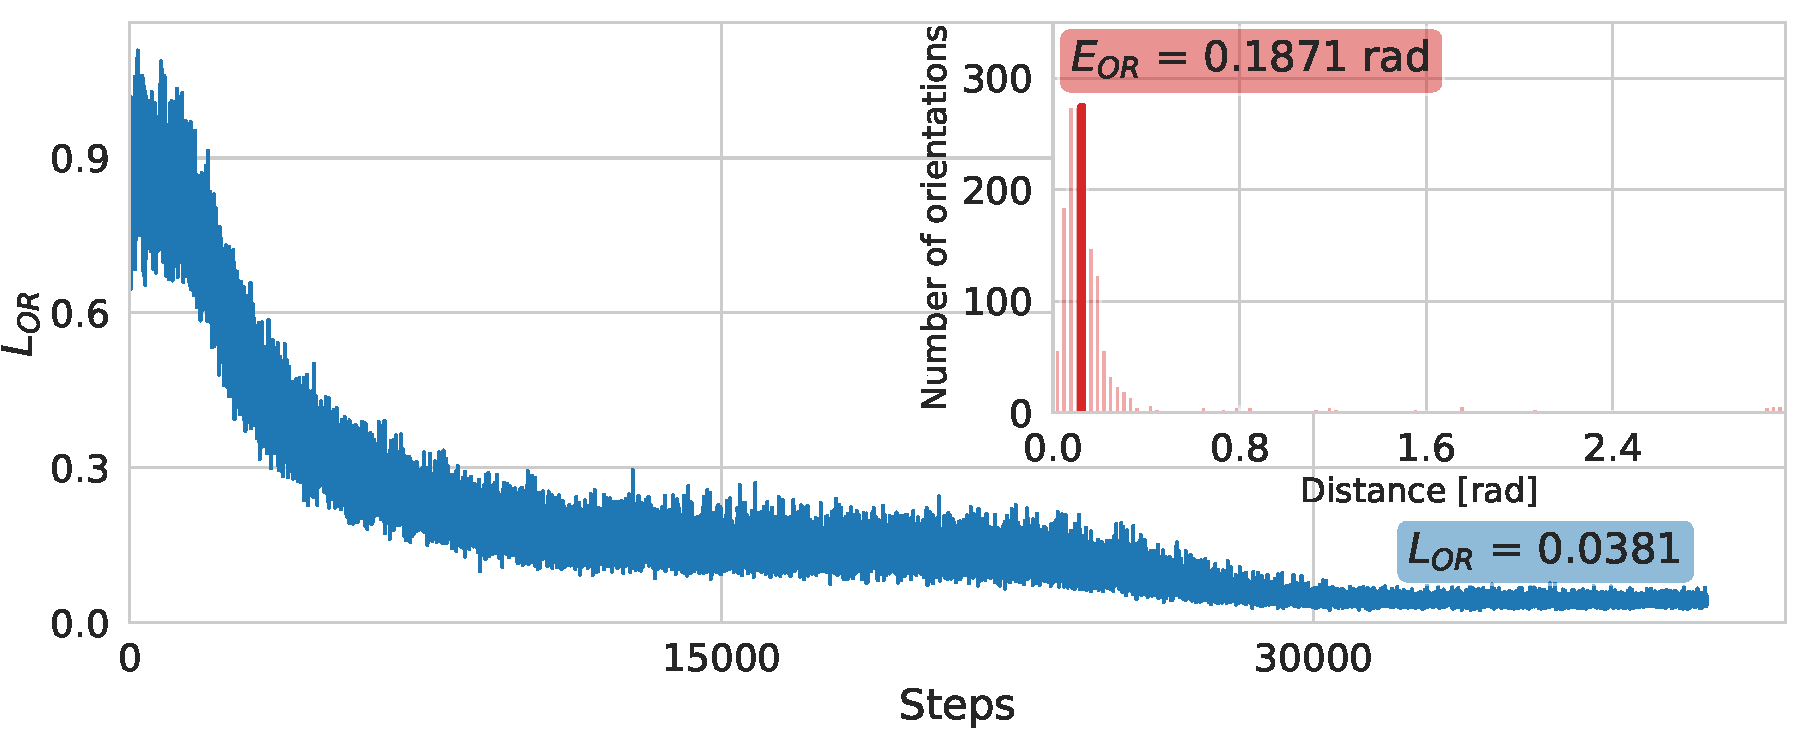
\includegraphics[height=5.5cm]{figures/5a1a_noise0_ar_aa}
        \caption{Recovery loss \eqnref{orientation-recovery} and recovery error \eqnref{orientation-recovery-error}.}
    \end{subfigure}
    \hfill
    \begin{subfigure}[b]{0.25\textwidth}
        \centering
        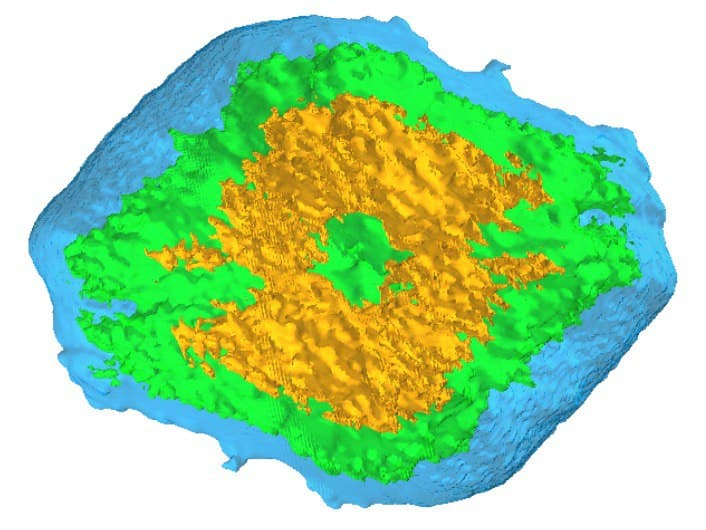
\includegraphics[width=0.99\linewidth]{figures/5a1a_ground_truth}
        \caption{Reconstruction from true orientations ${\big\{q_p\big\}}_{p=1}^P$.}
    \end{subfigure}
    % \\
    % \begin{subfigure}[b]{0.45\textwidth}
    %     \centering
    %     %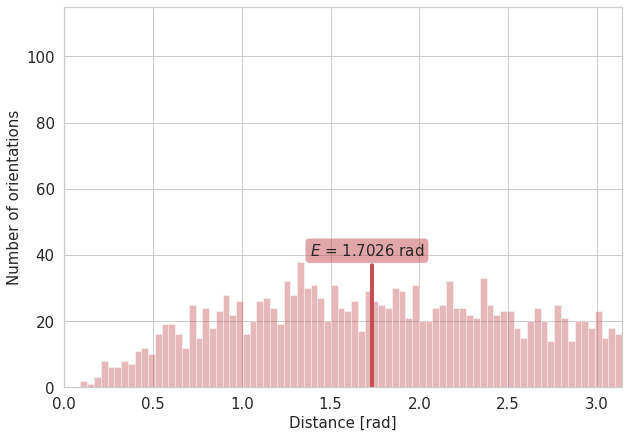
\includegraphics[height=5.7cm]{figures/5a1a_noise0_angle_alignment_before}
    %     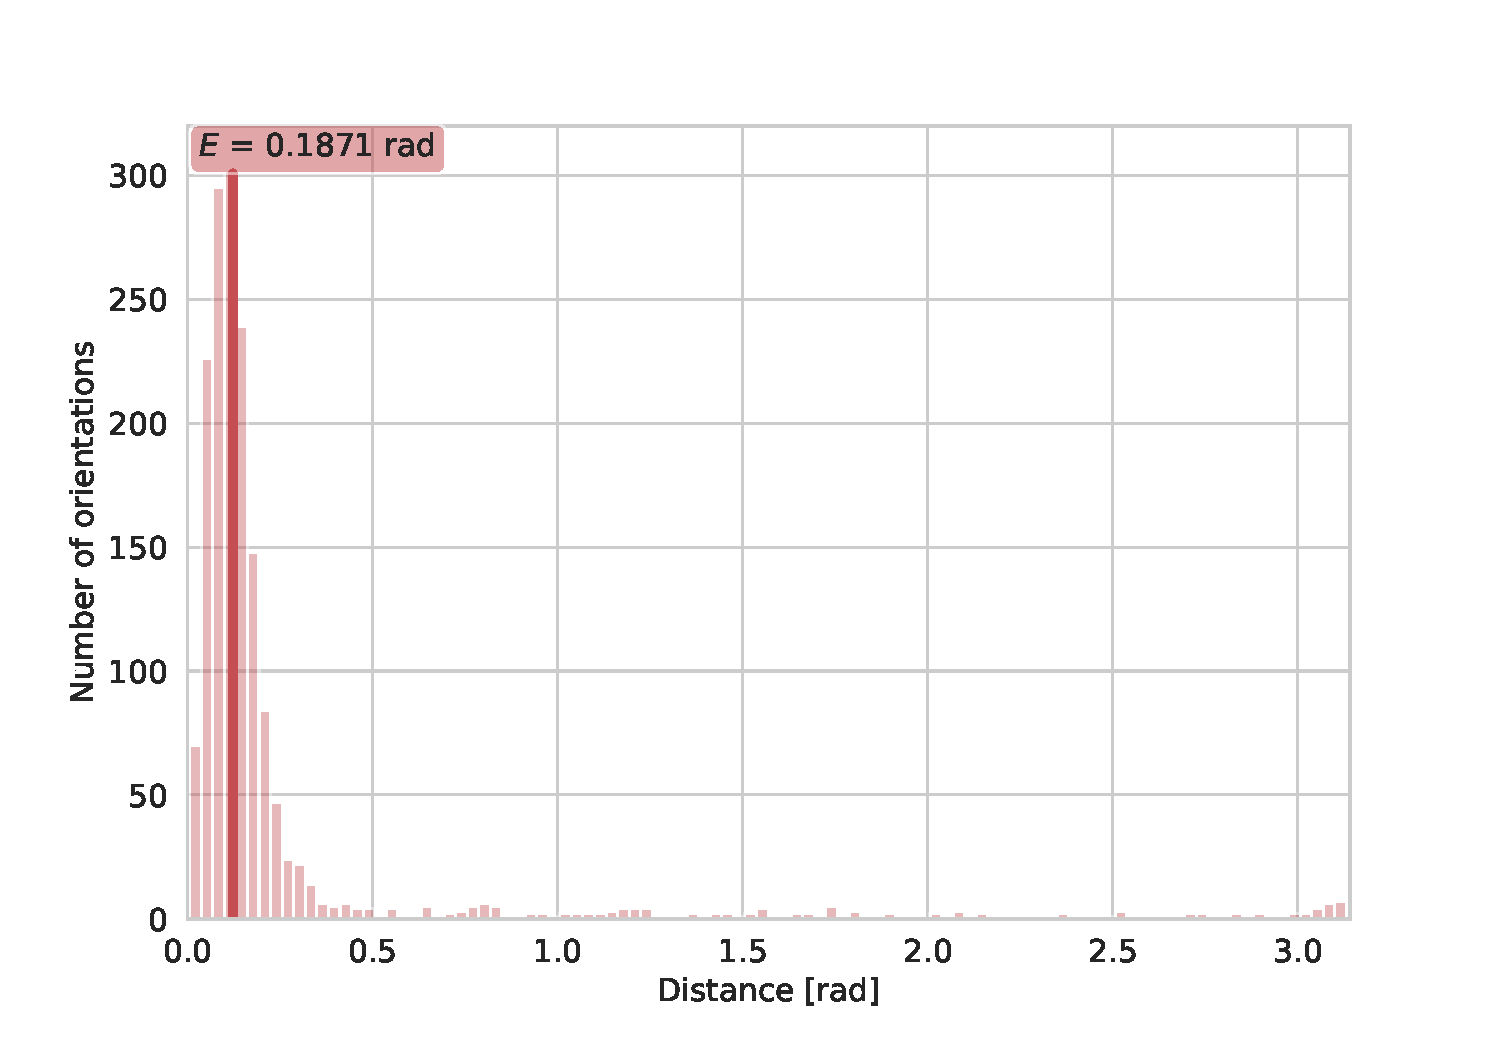
\includegraphics[height=5.5cm]{figures/5a1a_noise0_angle_alignment_after}
    %     \caption{Orientation recovery error \eqnref{orientation-recovery-error}.}
    % \end{subfigure}
    \hfill
    \begin{subfigure}[b]{0.25\textwidth}
        \centering
        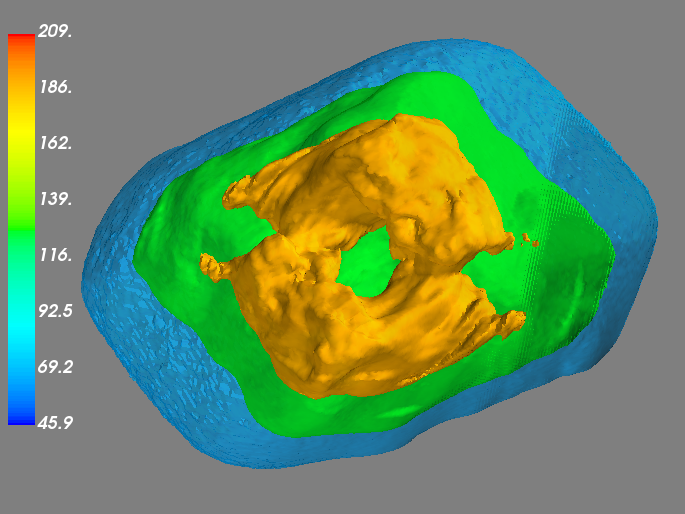
\includegraphics[width=0.99\linewidth]{figures/5a1a_aligned}
        \caption{Reconstruction from recovered orientations ${\big\{\widehat{q_p}\big\}}_{p=1}^P$.}
    \end{subfigure}
    \caption{
        Orientation recovery and reconstruction of the symmetric protein (\texttt{5a1a}) from noiseless projections.
    }\label{fig:5a1a-orientation-recovery-loss}
    \label{fig:angle-alignment-5a1a-noise0}
    \label{fig:5a1a-reconstruction-noise0}
\end{figure}

Lastly, we performed the protein reconstruction with the same ASTRA toolbox setting as for the asymmetric protein. 
The results of the reconstruction are shown in \figref{5a1a-reconstruction-noise0}.
We successfully reconstructed the symmetric protein even though the distance estimation was noisier than the one performed on the asymmetric protein.

We observe that the pipeline works, but for the state-of-the-art reconstruction we need a better distance estimation.
However, the method developed is promising since the learned distance is robust to perturbations.
We observe that the orientation recovery and distance estimation are interconnected, \textit{i.e.} if one works the other one will work.

To check the generalization to unseen proteins, and not only to  unseen projections, we trained the distance estimation on the set of four different proteins (\texttt{5nvu}~\cite{5nvu_pdb}, \texttt{5nvs}~\cite{5nvs_pdb}, \texttt{6mem}~\cite{6mem_pdb}, \texttt{6o1o}~\cite{6o1o_pdb}) that have the same type of symmetry (asymmetric  C1) as the one protein (\texttt{5j0n}) in the test dataset that is used in orientation recovery.
The orientation recovery reached the error of 0.0352.
This proves that distance learning was able to abstract the protein and that way generalized the distance metric to the unseen proteins.

\section{Discussion}\label{sec:discussion}

% Summary.
In this work, we explored the use of distance learning between pairs of 2D cryo-EM projections from a 3D protein structure to infer the unknown orientation at which each projection was imaged from.
Our two-step method relies on the training of a SiameseNN to estimate pairwise distances between unseen projections, followed by the recovery of the orientations from these distances through an appropriate minimization scheme.

The benefit of this approach, at least in theory, is that it would permit to estimate the unknown orientations in single-particle cryo-EM directly from the acquired dataset, \ie, without the need for intermediate reconstruction procedure or initial volume estimate; this has obvious useful implications in the field.

At the current stage of development, the method has been evaluated on synthetic datasets for two different proteins.
The results provide key insights on the viability of the proposed scheme.
First, they demonstrate that a SiameseNN can learn a distance function between projections that estimates the difference in their orientation (\secref{results:distance-estimation:learned}) and that is invariant to off-centering shifts and robust to increasing levels of noise (\secref{results:distance-estimation:sensitivity})---an important feat in cryo-EM\@.
\mdeff{The two phrases in the following sentence sound redundant.}
Second, they guarantee that an accurate distance estimation leads to a correct recovery of the orientations, while providing indications that the quality of this recovery depends on the precision of the estimated distances (\secref{results:orientation-recovery:sensitivity}, \secref{results:distance-estimation:sensitivity}).
\todo{Finally, our method was able to recover orientations with an error of $0.20$ to $0.25$ radians ($11$ to $14\degree$) from noiseless and noisy projections---leading to an initial volume/reconstruction with a resolution of $???$ (\secref{results:orientation-recovery:reconstruction}).}
All in all, the estimation of more accurate distances leads to the recovery of more accurate orientations which leads to the reconstruction of a more accurate initial volume.

% Future work.
While the method is not yet at the stage where it can be deployed in practice, we believe that a series of developments could help it become a relevant contributor for single-particle cryo-EM reconstruction.%
\footnote{Note that the present project will not be further continued by its authors due to other professional occupations. Hence, we strongly encourage you to build on these ideas and hopefully make it a practical tool.}
As previously discussed, the results underline the importance of learning an accurate distance estimator. % $\widehat{d_p}$.
In this regard, the performance of the SiameseNN could be improved in several ways.
% Method gains: mostly distance learning maybe recovery (not alignment).
%A set of additional technical developments could also further improve performance.
First, the architecture of the SiameseNN's twin CNNs should be expanded and tuned.
% , as well as the distance metric between the two CNN outputs.
% For instance, one could parametrize the function $d_f$---which compares the similarity of the features outputs (see \figref{schematic:distance-learning})---as a feed-forward neural network instead of the current Euclidean distance, and learn its weights as well.
Second, the training of the SiameseNN could be improved, perhaps by providing more supervision by separately predicting the differences in direction $(\theta_2,\theta_1)$ and in-plane angle $\theta_3$.
% \mdeff{Let's ignore improvements to recovery and concentrate the story on better distance learning -> better recovery -> better reconstruction.}
%Among others, one shall explore whether reducing the influence of larger distances in orientation recovery could bring further gain in accuracy.
% \mdeff{The following are issues with alignment---not directly related to our method---that we mentioned elsewhere.}
% Angle alignment didn't always work, even when $L_\text{OR}$ was low (examples?): We might miss a transformation in \eqnref{orientation-recovery-error}.
% Why did we need to align with \eqnref{orientation-recovery-error} before reconstructing with ASTRA\@?

% Data gains.
Importantly, the SiameseNN would be better trained on a more exhaustive and diverse cryo-EM dataset.
Indeed, the success of the SiameseNN as a faithful estimator of relative orientations eventually relies on our capacity to generate a synthetic training dataset whose data distribution is diverse enough to cover that of unseen projection datasets.
Such realistic cryo-EM projections could be generated by relying on a more expressive formulation of the cryo-EM physics and taking advantage of the thousands of atomic models available in the PDB\@.
% \mdeff{PDB database sounds redundant as PDB stands for protein database.}
In particular, a necessary extension will be to include the effects of the PSF when generating training data and evaluate its impact on the SiameseNN\@. % like we did for shifts and noise

% Towards practical use: unseen proteins (also data) and real measurements.
A final phase of tests before deploying the method on real cryo-EM measurements will be to extensively test the method on ``unseen proteins'', \ie, proteins whose simulated projections have never been seen by the SiameseNN\@.
Early experiments indicate the feasibility of this enterprise (see \apxref{unseen-proteins}).
In this regard, an interesting aspect of our method is that the twin CNNs within the SiameseNN intrinsically predict the \textit{relationship} between projections, allowing the SiameseNN as a whole to abstract the particular volume.
%Consequently, a well-trained distance estimator could be relatively robust to the ``mismatch'' of volumes within the training set.
%In the same line of thought,
Learning benefits from the profound structural similarity shared by proteins---after all, they are all derived from the same $21$ building blocks.
% Learning exploits statistical effects, given here by biological building block.

% \mdeff{I propose to omit the following sentence (which is a truism and is stated in the previous paragraph) to finish on a more forceful note.}
% Eventually, the performance of the method on real cryo-EM measurements will provide the real measure of its potential, the imaging conditions being notoriously challenging in single-particle cryo-EM\@.
% Further down the line and still in the real of the hypothetical, new approaches for the training of the SiameseNN able to handle the handling of proteins with multiple conformational states could be explored.


\section*{Acknowledgements}

Grants to acknowledge? \lau{I need to check with MU on my side.}

The authors are thankful to Dr. Matthieu Simeoni and Dr. Julien Fageot for insightful mathematical discussions throughout the project. 





\bibliographystyle{IEEEtran}
\bibliography{refs}

%\clearpage

% \section{Different performance metrics}\label{apx:metrics-review}

% \todo{Keep? Review and copy-edit necessary.}

% There are many different ways of evaluating the pipeline performance found in the field of pose estimation. Some of the evaluations include the following:
% \begin{itemize}
% \item Intersection over Union (IoU) of the object 3D cloud with a custom threshold classifying it as a good estimate or not (\eg, in the paper~\cite{10.1007/s11263-014-0733-5} the threshold score above 0.5 is considered good estimation).
% \item Translation and rotation error between estimated 3D model and true 3D model with fixed thresholds (\eg, in the paper~\cite{shotton2013scene} they require the translation error to be below 5 cm and rotation error to be below 5\degree)
% \item The average distance of all the points of the model from their transformed version, and if the error is less than the constant multiple of diameter of the 3D model, it is considered correctly evaluated (\eg, evaluation error is used in papers~\cite{10.1007/978-3-642-37331-2_42, xiang2018posecnn})
% \item Reprojection error that projects the estimated points onto the image and computes the pairwise distances in the image space, instead of computing distances in the 3D model space (\eg, used in paper~\cite{xiang2018posecnn})
% \item The recovery error measured as Frobenius norm from estimated 3D model and true model, where 3D model is composed of 3D locations of important landmarks (\eg, elbow for human pose estimation)~\cite{wangni2018monocular}
% \item Average Orientation Similarity (AOS) is the difference between the true and estimated model with a cosine similarity term~\cite{RedondoCabrera2016PoseEE}
% \item Mean Angle Error (MAE) and Median Angle Error (MedError) evaluated and compared with other pose estimation error metrics in the paper~\cite{RedondoCabrera2016PoseEE}.
% \end{itemize}

\section{Proteins and their projections}\label{apx:proteins-and-their-projections}
\begin{figure}[ht!]
    \centering
    \begin{minipage}[b]{0.51\linewidth}
        \centering
        \begin{subfigure}[b]{0.49\linewidth}
            \centering
            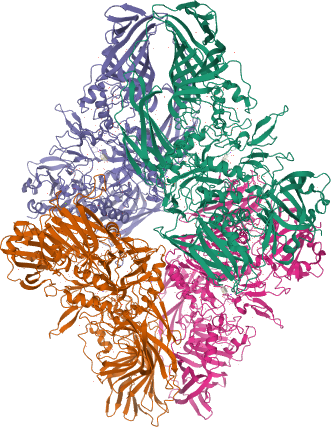
\includegraphics[height=3cm]{figures/5a1a_pdb.png}
            \caption{Atomic model of \texttt{5a1a}.}
        \end{subfigure}
        \hfill
        \begin{subfigure}[b]{0.49\linewidth}
            \centering
            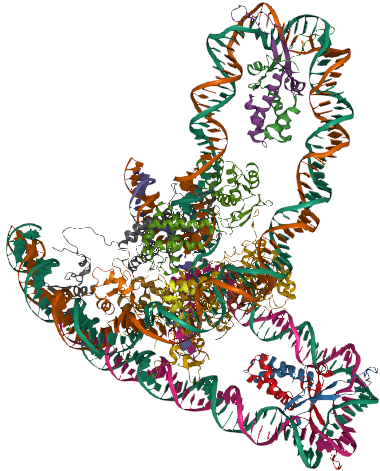
\includegraphics[height=3cm]{figures/5j0n_pdb_.png}
            \caption{Atomic model of \texttt{5j0n}.}
        \end{subfigure}
        \\ \vspace{0.5em}
        \begin{subfigure}[b]{0.49\linewidth}
            \centering
            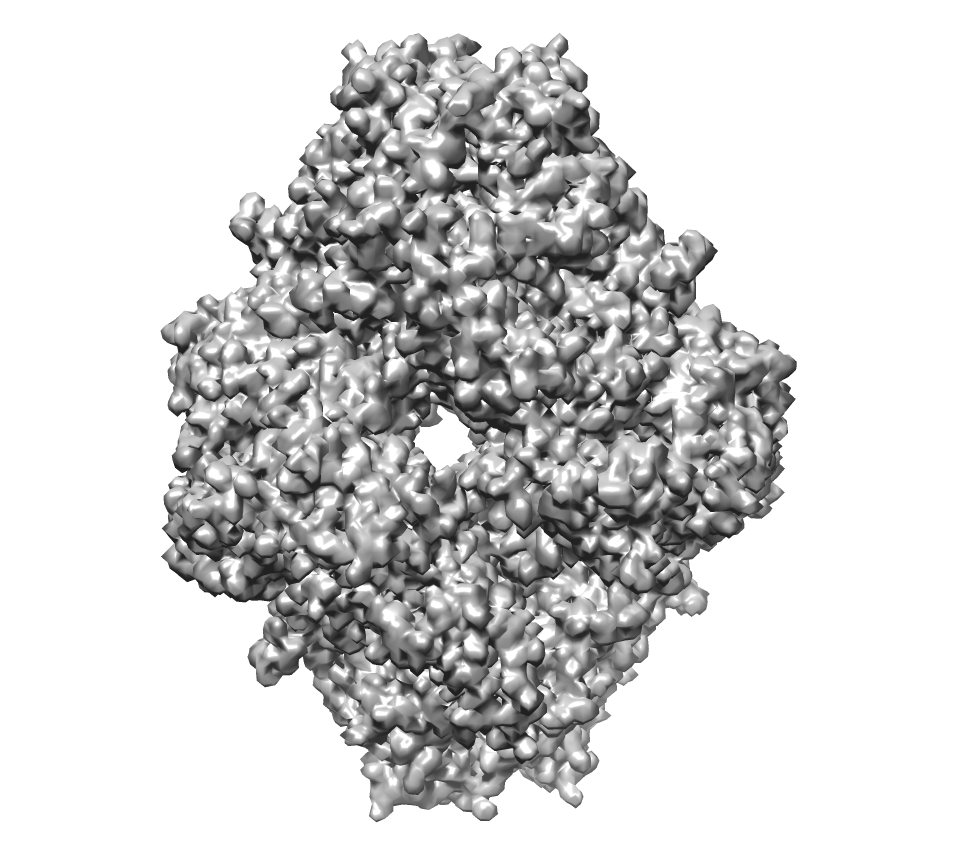
\includegraphics[height=3cm]{figures/5a1a_5A.png}
            \caption{1\AA\ density map $\x$ of \texttt{5a1a}.}%
            \label{fig:density-map:5j0n:ground-truth}
        \end{subfigure}
        \hfill
        \begin{subfigure}[b]{0.49\linewidth}
            \centering
            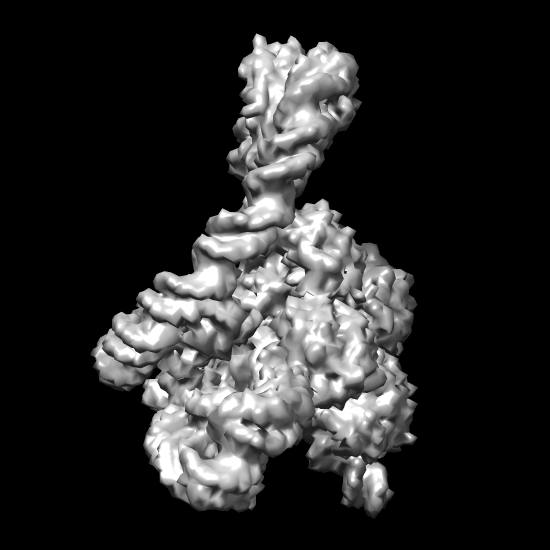
\includegraphics[height=3cm]{figures/5j0n_5A.png}
            \caption{3.67\AA\ density map $\x$ of \texttt{5j0n}.}
        \end{subfigure}
        \caption{%
            %A D2 symmetric (\texttt{5a1a}) and an asymmetric (\texttt{5j0n}) protein.
            Two proteins with different symmetries.
            %The $\beta$-galactosidase (\texttt{5a1a}) and the lambda excision HJ intermediate (\texttt{5j0n}).
        }\label{fig:pdb-proteins}
    \end{minipage}
    \hfill
    \begin{minipage}[b]{0.48\linewidth}
        \centering
        \begin{subfigure}[b]{0.49\linewidth}
            \centering
            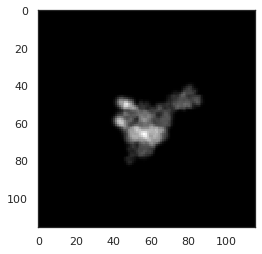
\includegraphics[height=3cm]{figures/5j0n_noise0}
            \caption{$\p = \mathbf{P}_{\bth} \mathbf{x}$}
        \end{subfigure}
        \hfill
        \begin{subfigure}[b]{0.49\linewidth}
            \centering
            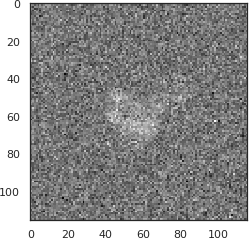
\includegraphics[height=3cm]{figures/5j0n_noise16}
            \caption{$\p = \mathbf{P}_{\bth} \mathbf{x} + \mathbf{n}$}
    %, \; \mathbf{n} \sim \mathcal{N}(0, 16\mathbf{I})$}
        \end{subfigure}
        \\ \vspace{0.5em}
        \begin{subfigure}[b]{0.49\linewidth}
            \centering
            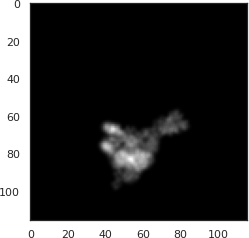
\includegraphics[height=3cm]{figures/5j0n_translated}
            \caption{$\p = \mathbf{S}_{\mathbf{t}} \mathbf{P}_{\bth} \mathbf{x}$}
        \end{subfigure}
        \hfill
        \begin{subfigure}[b]{0.49\linewidth}
            \centering
            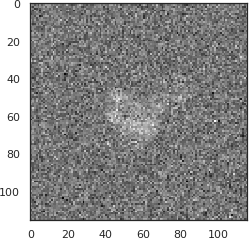
\includegraphics[height=3cm]{figures/5j0n_noise16_translated}
            \caption{$\p = \mathbf{S}_{\mathbf{t}} \mathbf{P}_{\bth} \mathbf{x} + \mathbf{n}$}
        \end{subfigure}
        \caption{%
            Example projections of \texttt{5j0n} ($\mathbf{n} \sim \mathcal{N}(0, 16\mathbf{I})$).
            % (a)~unperturbed, (b)~noisy, (c)~shifted, (d)~noisy and shifted.
        }\label{fig:different-projections}
    \end{minipage}
\end{figure}


%%%%%%%%%%%%%%%%%%%%%%%%%%%%%%%%
\section{Sampling of orientations}\label{apx:orientation-sampling}

%\todo{What do we want to say here? Sampling of orientations, or sampling of distances?}

\figref{orientation-sampling} shows four distributions of orientations and the distributions of distances they induce.
%While the distributions distances for partial coverages of directions flatten (compared with both full direction coverage), the shorter distances are still under-sampled.
As shorter distances are under-sampled, we uniformly resampled the distances to avoid biasing the training of our distance estimator.

While we control the distributions of orientations and distances to facilitate distance learning, we cannot control them when recovering orientations of a given set of projections.
Comparing Figure~\ref{fig:nonuniform:recovery} with~\ref{fig:5j0n-noise0-orientation-recovery}, and~\ref{fig:nonuniform:reconstruction} with~\ref{fig:5j0n-reconstruction-fsc}, shows that the recovered orientations and the reconstructed density are barely affected by a non-uniform sampling of orientations---a condition that might happen in real cryo-EM acquisitions.

%\banjac{I remember putting somewhere that we have support for both, but I don't see it. I can put a histogram and respective $S^2$ space visualization in the appendix that will visualize the difference. Why we used it? From the log I see that OR was not converging to 0 so we thought is is because we have underestimated learned distance. Shortly after, the OR started working and we didn't continue further with this idea.}

\begin{figure}[ht!]
    \centering
    \begin{minipage}{.33\linewidth}
        \begin{subfigure}[b]{\linewidth}
            \centering
            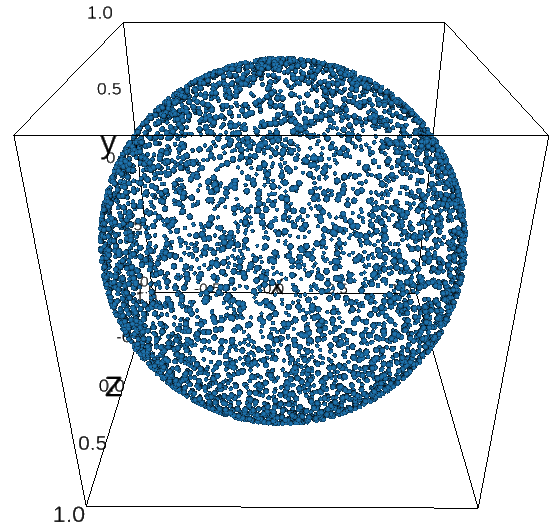
\includegraphics[height=2.5cm]{figures/uniform_quaternion.png}%
            \hfill
            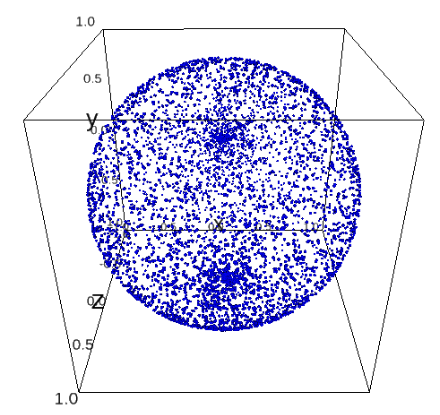
\includegraphics[height=2.5cm]{figures/uniform_angles.png}
            \\ \vspace{0.2cm}
            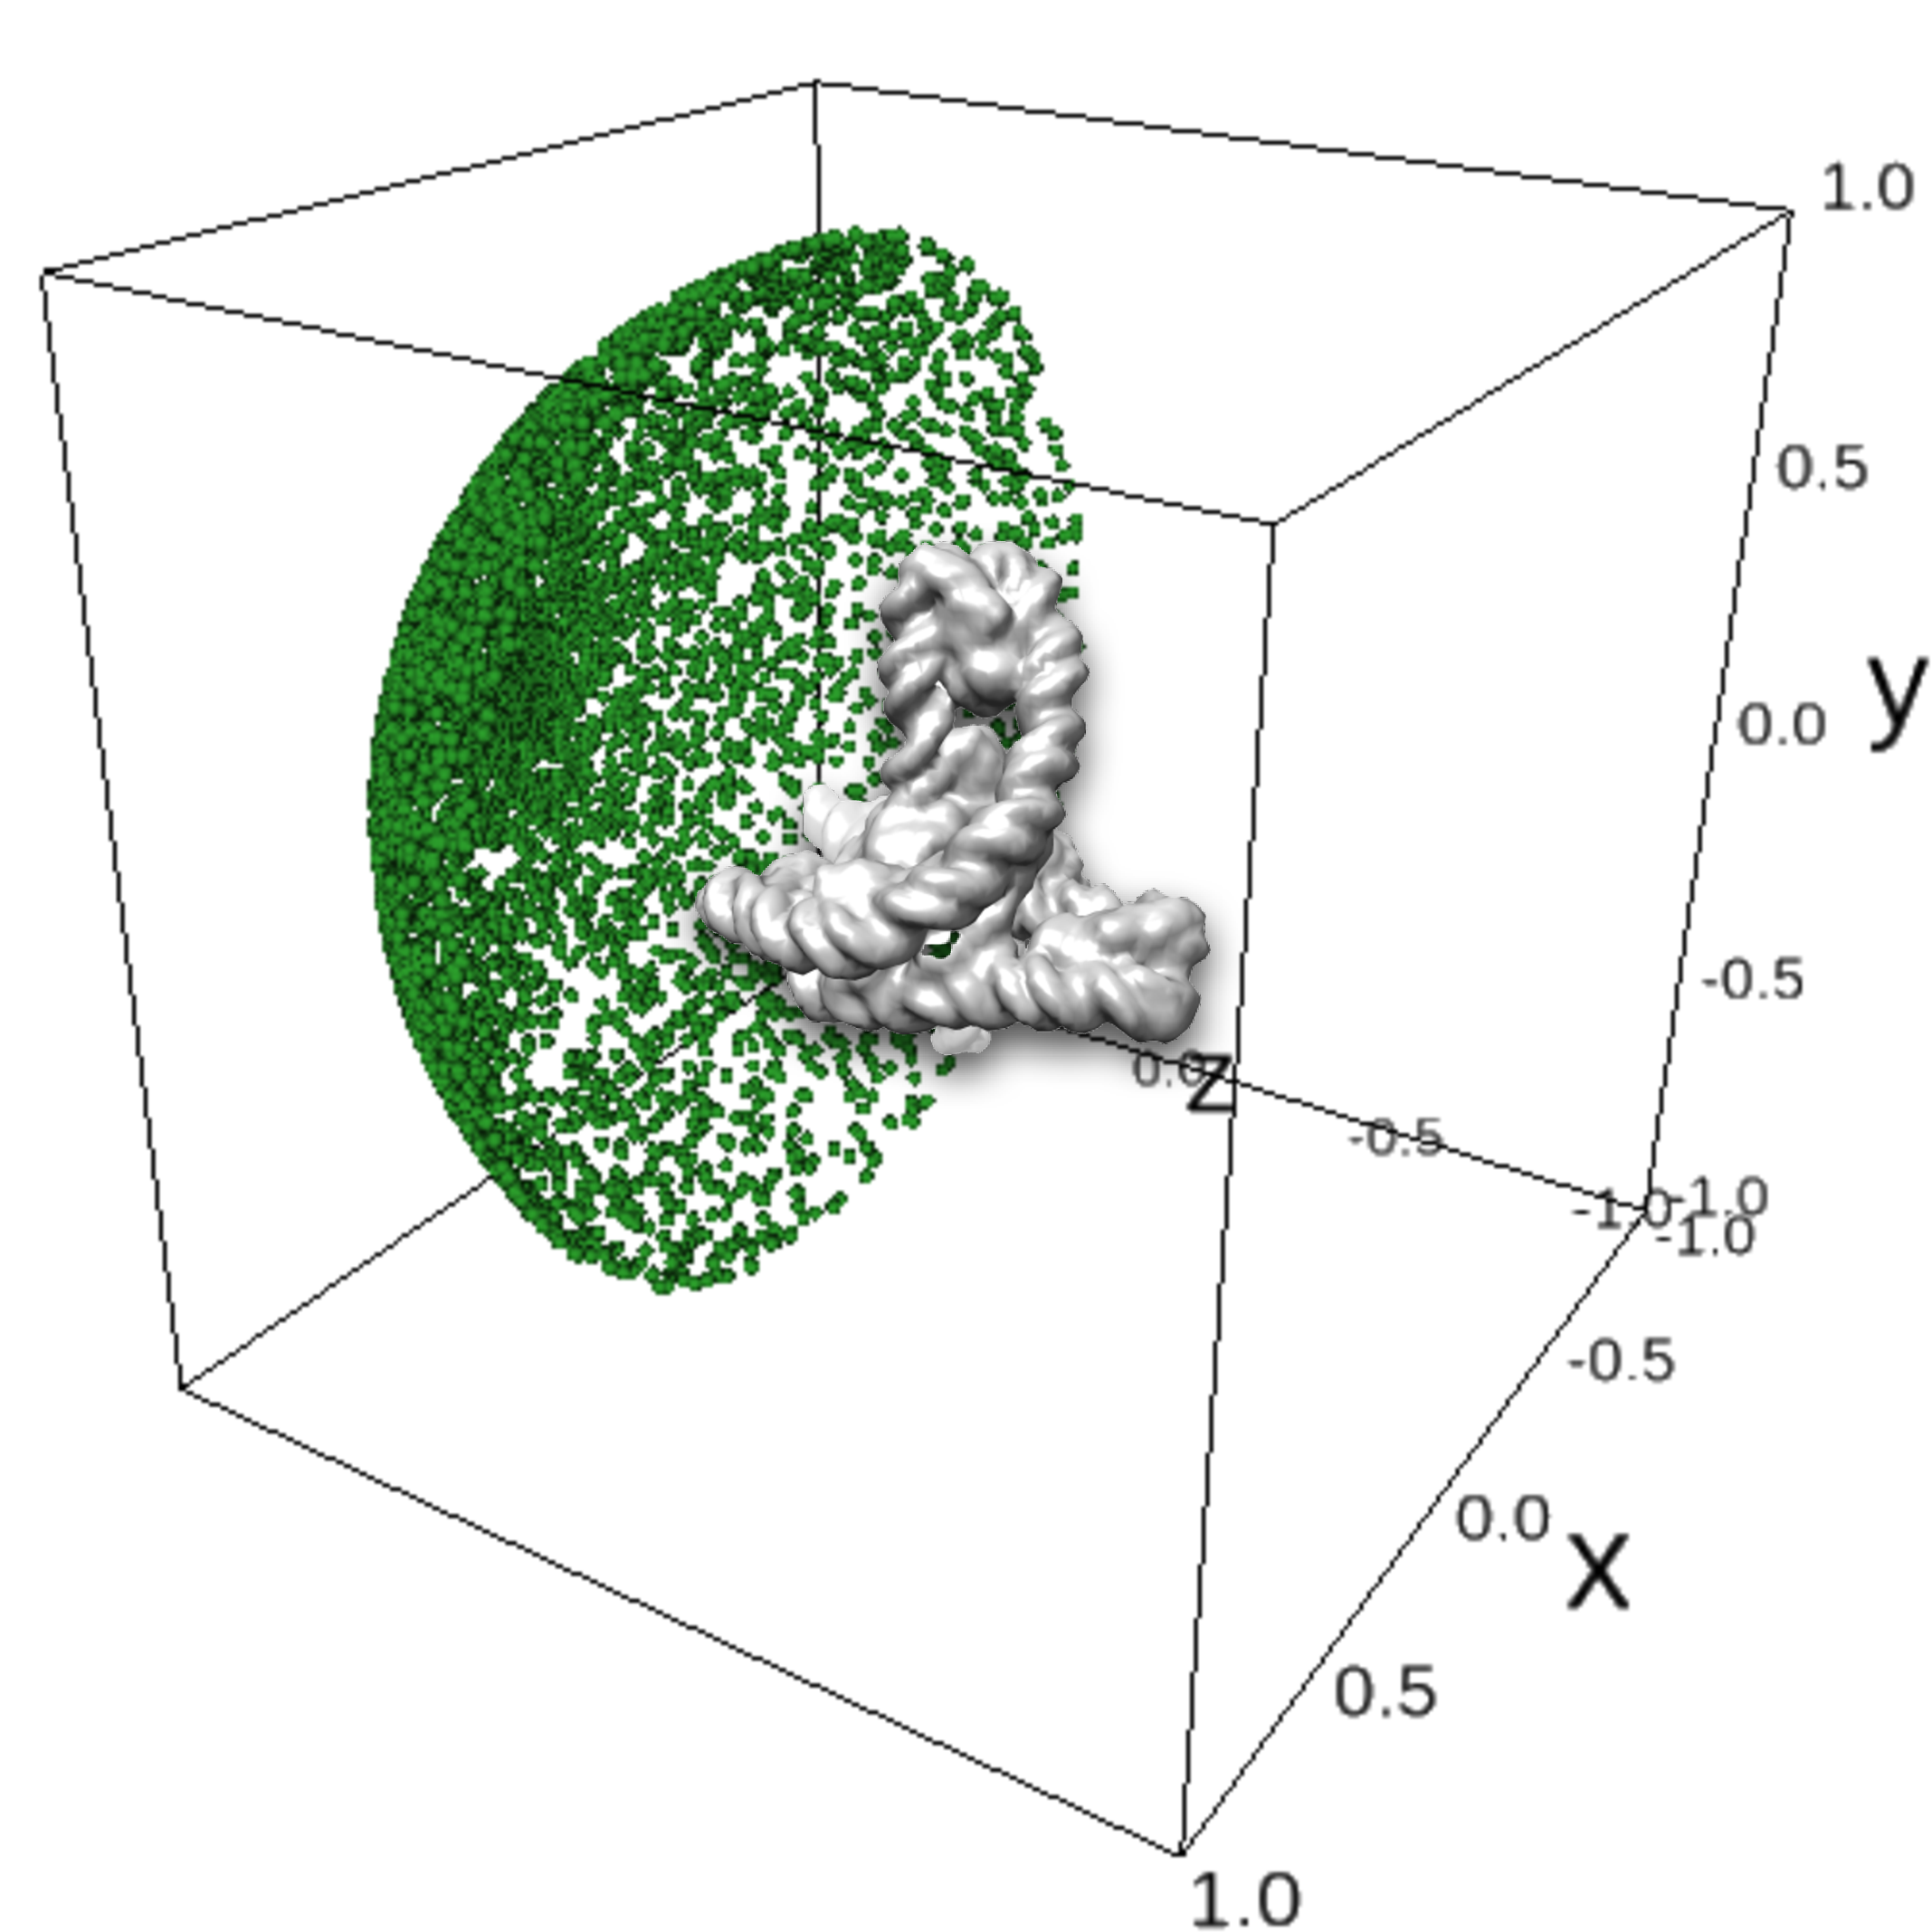
\includegraphics[height=2.5cm]{figures/5j0n-cvg2.pdf}
            \hfill
            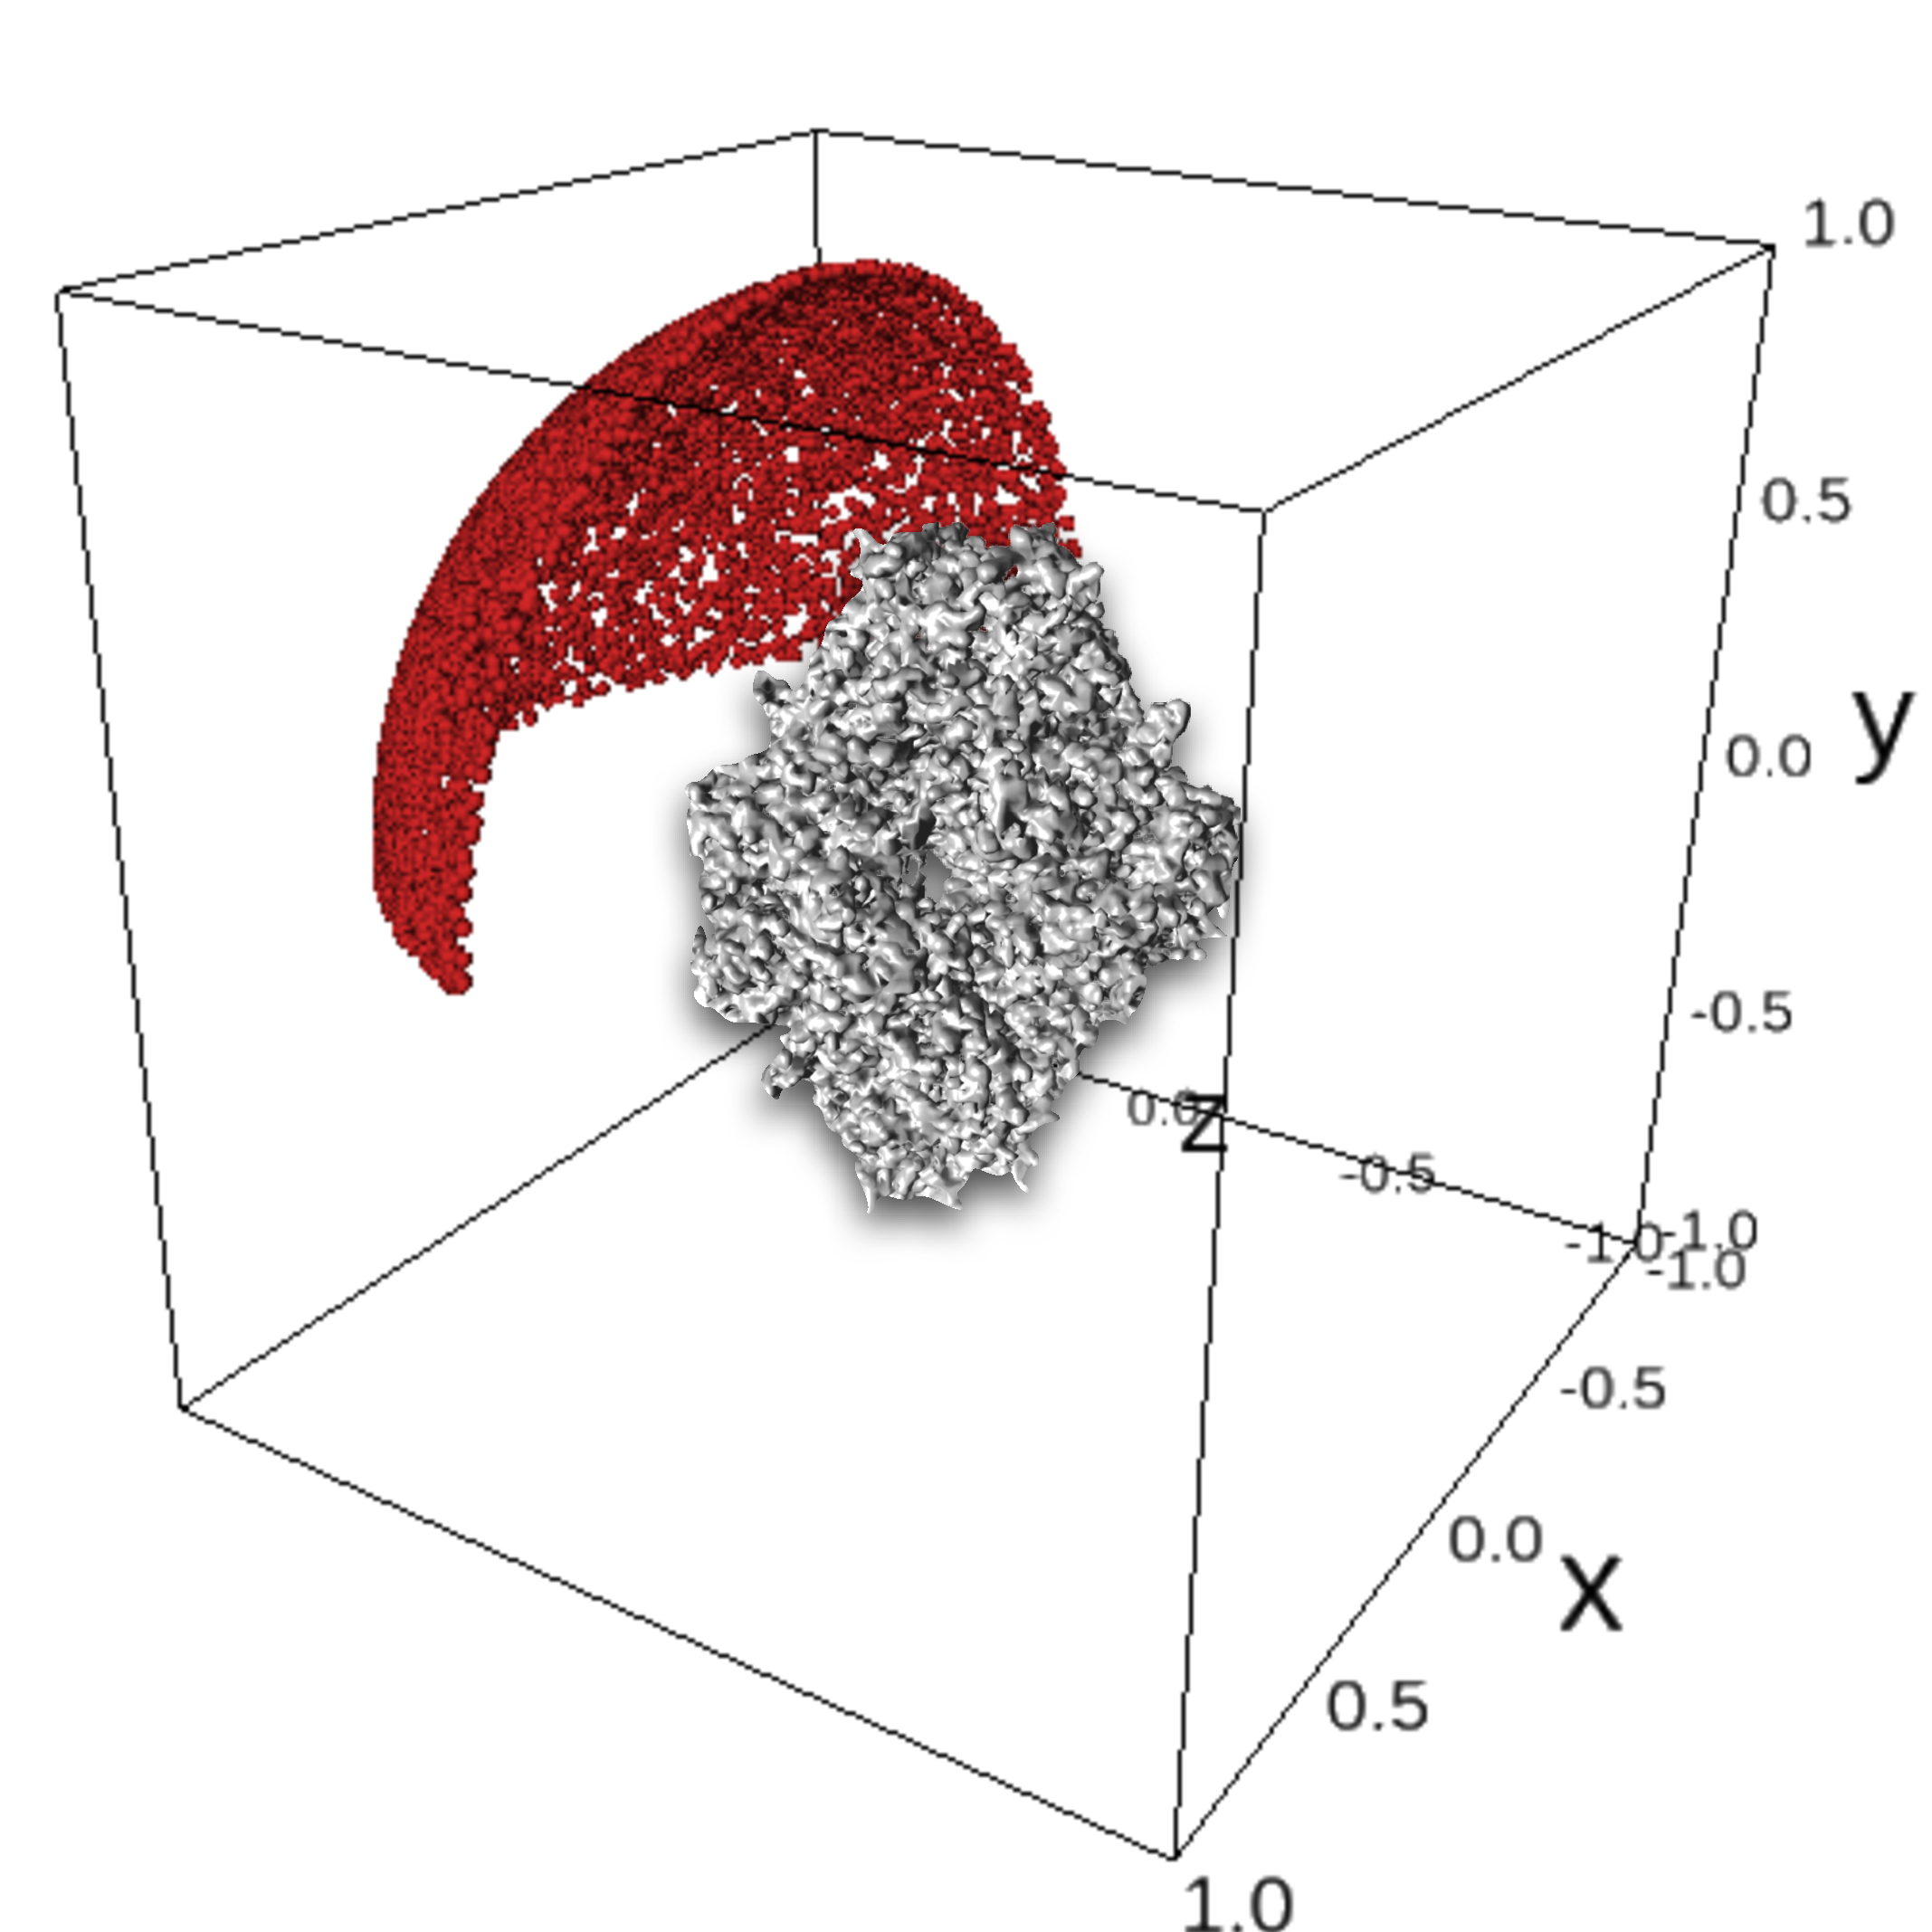
\includegraphics[height=2.5cm]{figures/5a1a-cvg2.pdf}
            \caption{Sampled directions $(\theta_2, \theta_1)$.}%
            \label{fig:orientation-sampling:directions}
        \end{subfigure}
    \end{minipage}
    \hfill
    \begin{minipage}{.65\linewidth}
        \begin{subfigure}[b]{0.37\linewidth}
            \centering
            % 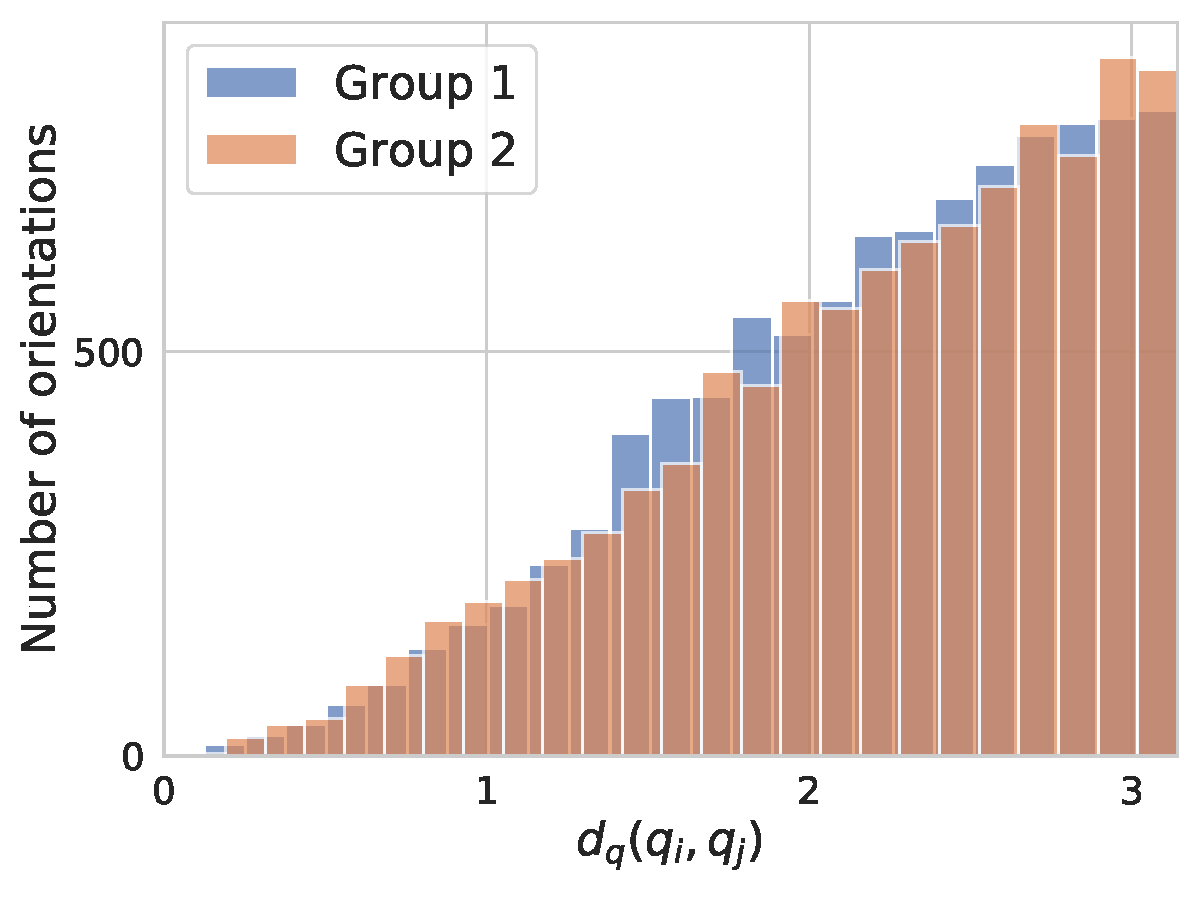
\includegraphics[height=8em]{figures/dQ_5j0n_uniform_quaternions_vs_angles.pdf}
            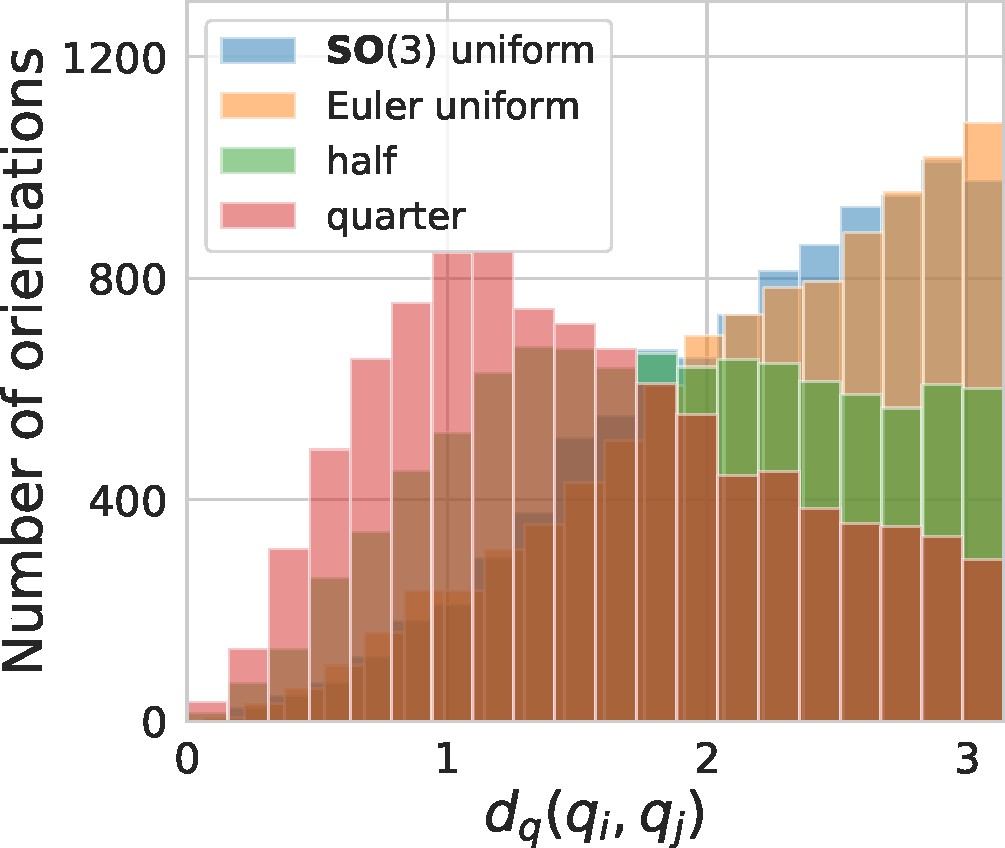
\includegraphics[height=2.4cm]{figures/dQ_distribution_coverage.pdf}
            \caption{Distribution of distances $d_q$.}%
            \label{fig:orientation-sampling:distances}
            \vspace{0.2cm}
        \end{subfigure}
        \hfill
        \begin{subfigure}[b]{0.6\linewidth}
            \centering
            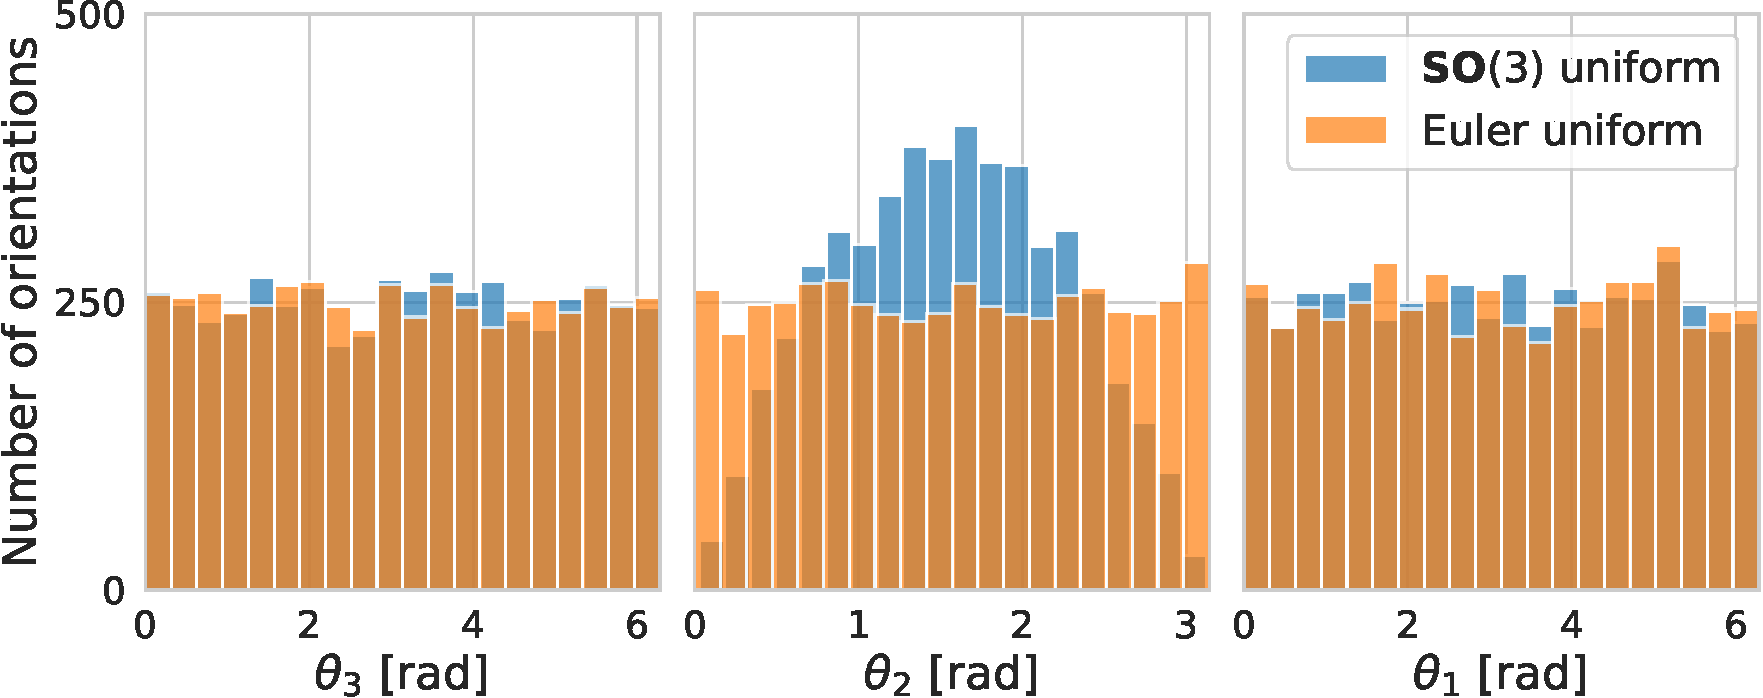
\includegraphics[height=2.4cm]{figures/uniform_quaternions_vs_angles_ang.pdf}
            \caption{Distribution of Euler angles $\bth = (\theta_3,\theta_2,\theta_1)$.}%
            \label{fig:orientation-sampling:angles}
            \vspace{0.2cm}
        \end{subfigure}
        \begin{subfigure}[b]{0.97\linewidth}
            \centering
            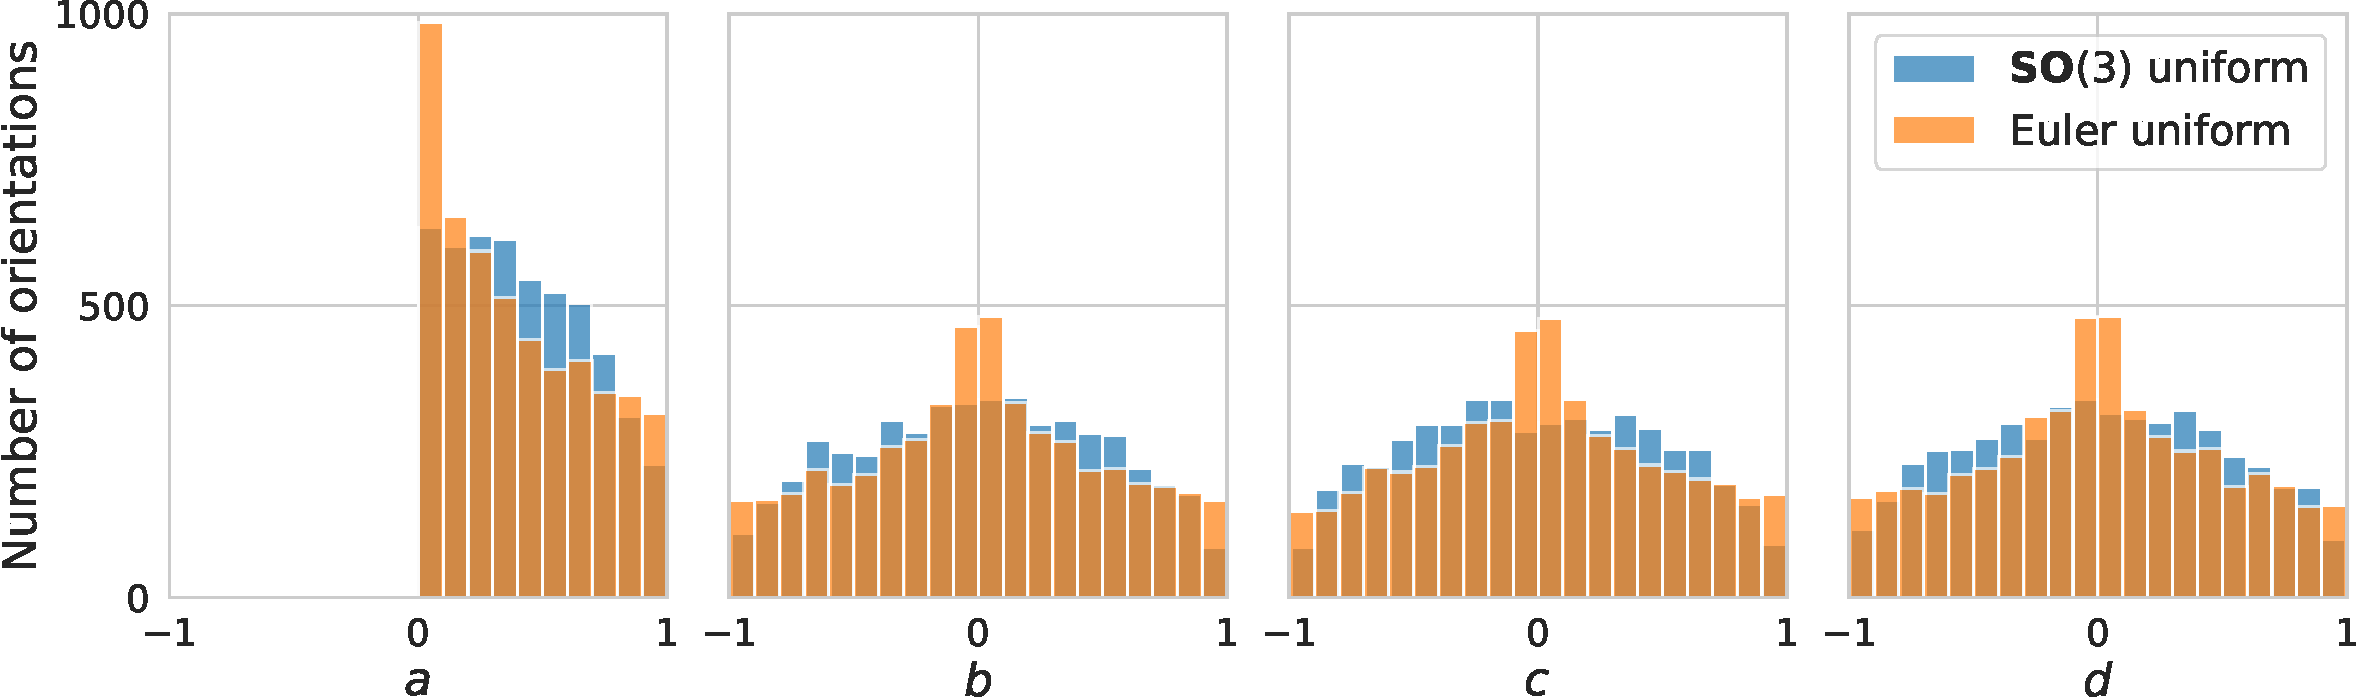
\includegraphics[height=2.4cm]{figures/uniform_quaternions_vs_angles_q.pdf}
            \caption{Distribution of quaternions $q = a + b\boldsymbol{i} + c\boldsymbol{j} + d\boldsymbol{k}$.}%
            \label{fig:orientation-sampling:quaternions}
        \end{subfigure}
    \end{minipage}
    \caption{%
        % ($P < 10,000$)
        Sampling of orientations from four distributions:
        %illustrating their constrained range, and the distances they induce:
        (blue) uniform on $\SO(3)$, (orange) uniform on Euler angles, (green) Euler uniform restricted to half the directions $(\theta_2, \theta_1) \in [0,\frac{\pi}{2}[ \, \times \, [0,2\pi[$, and (red) $\SO(3)$ uniform restricted to a quarter of the directions $(\theta_2, \theta_1) \in [0,\frac{\pi}{2}[ \, \times \, [0,\pi[$.
    }\label{fig:orientation-sampling}
\end{figure}

\begin{figure}[ht!]
    \centering
    \begin{subfigure}[b]{0.48\linewidth}
        \centering
        % \includegraphics[height=3cm]{figures/5j0n_ar_aa_fullcvg.pdf}
        \includegraphics[height=3cm]{figures/5j0n_ar_aa_fullcvg_smaller.pdf}
        \caption{Distance learning and orientation recovery.}%
        \label{fig:nonuniform:recovery}
    \end{subfigure}
    \hfill
    \begin{subfigure}[b]{0.48\linewidth}
        \centering
        % \includegraphics[height=4cm]{figures/FSC_5j0n_fullcvg_noise0_fin_vs_init.pdf}
        \includegraphics[height=3cm]{figures/5j0n_fullcvg_noise0_FSC_apr_init_customFSC.pdf}
        \caption{The FSC of the reconstructed density.}%
        \label{fig:nonuniform:reconstruction}
    \end{subfigure}
    \caption{%
        Orientation recovery and density reconstruction from noiseless projections of \texttt{5j0n} acquired from non-uniformly sampled orientations (uniformly sampled Euler angles, \figref{orientation-sampling} (orange)).
        %Full pipeline on the orientations with uniform sampling of Euler angles from full 2-sphere coverage.
    }
\end{figure}

\section{Orientation recovery from exact distances}\label{apx:results:orientation-recovery:exact}

%\mdeff{Story: works perfectly despite no convexity guarantee and sampling.}

To verify that the lack of a convexity guarantee for \eqnref{orientation-recovery} and the sampling of the sum are non-issues in practice, we attempted orientation recovery under exact distance estimation $\widehat{d_p}(\p_i, \p_j) = d_q(q_i, q_j)$.
Orientations were perfectly recovered;
\figref{5j0n-orientation-recovery-loss} shows the convergence of $L_\text{OR}$ to zero.
\figref{5j0n-aa-loss-perfect-distances} shows how~\eqnref{orientation-recovery-error} could then perfectly align the recovered and true orientations---leading to $E_\text{OR} = 0$.
It illustrates how alignment is necessary to evaluate the performance of orientation recovery.

\begin{figure}[ht!]
    \begin{minipage}[t]{0.30\linewidth}
        \centering
        %\includegraphics[height=3cm]{figures/5j0n_perfect_angle_recovery}
        % \includegraphics[height=3cm]{figures/5a1a_quartercov_uniformS2_halfInplane_ar_aa}
        \includegraphics[height=3cm]{figures/5a1a_quartercov_uniformS2_perfect_ar_aa}
        \caption{%
            Example of perfect orientation recovery (for \texttt{5a1a}).
            The loss $L_\text{OR}$ \eqnref{orientation-recovery} converges to zero when the distance estimation is perfect, \ie, $\widehat{d_p}(\p_i, \p_j) = d_q(q_i, q_j)$.
            %\todo{Update to full in-plane.}
        }\label{fig:5j0n-orientation-recovery-loss}
    \end{minipage}
    \hfill
    \begin{minipage}[t]{0.66\linewidth}
%        \begin{subfigure}[b]{0.19\linewidth}
%            \centering
%            \includegraphics[height=3cm]{figures/5j0n_perfect_angle_ralignment_after}
%            \caption{Orientation recovery error with alignment.}
%        \end{subfigure}
%        \hfill
        % \begin{subfigure}[t]{4.3cm}
        %     \centering
        %     %\includegraphics[height=3cm]{figures/5j0n_perfect_angle_ralignment_before}
        %     \includegraphics[height=3cm]{figures/5a1a_quartercov_uniformS2_halfInplane_before_alignment}
        %     \caption{Error histogram $\{ d_q (q_i, \widehat{q_i}) \}$, \ie, before alignment.}
        % \end{subfigure}
        % \hfill
        \begin{subfigure}[t]{0.49\linewidth}
            \centering
            % \includegraphics[height=3cm]{figures/coverage_alignment_before.png}
            %\includegraphics[height=3cm]{figures/before_aa.png}
            \includegraphics[height=3cm]{figures/BeforeAA.pdf}
            \caption{Orientations before alignment.}
        \end{subfigure}
        \hfill
        \begin{subfigure}[t]{0.49\linewidth}
            \centering
            % \includegraphics[height=3cm]{figures/coverage_alignment_after.png}
            %\includegraphics[height=3cm]{figures/after_aa.png}
            \includegraphics[height=3cm]{figures/AfterAA.pdf}
            \caption{Orientations after alignment.}
        \end{subfigure}
        \caption{%
            Example of perfect alignment~\eqnref{orientation-recovery-error} after a perfect recovery~\eqnref{orientation-recovery}.
            The red histogram shows the errors (a) $\{d_q(q_i, \widehat{q_i})\}$ and (b) $\{d_q(q_i, \T \widehat{q_i})\}$, with the mean $E_\text{OR}$ highlighted.
            % and $\T$ as the optimum of \eqnref{orientation-recovery-error} on the right.
            True (green) and recovered (green) directions are shown in the insert.
            While both colors are seen in (b), they are superimposed.
        }\label{fig:5j0n-aa-loss-perfect-distances}
    %    \label{fig:angle-alignment-perfect}
    \end{minipage}
\end{figure}

\section{Euclidean distance between projections}\label{apx:results:distance-estimation:euclidean}

%\mdeff{Story: simplest baseline estimator, $d_{pe}$ somewhat estimates $d_q$, quickly plateaus (even in the simplest noiseless and centered case).
%Note the difference between symmetric and asymmetric proteins.}

We evaluate $\widehat{d_p}(\p_i, \p_j) = \| \p_i - \p_j \|_2$ (\ie, the Euclidean distance) as a baseline distance estimator.
\figref{euclidean-not-robust} shows the relationship between $\widehat{d_p}$ and $d_q$.
Two main observations can be made from this experiment.
First, as suspected, $\widehat{d_p}$ fails to be a consistent predictor of $d_q$, even in the simple imaging conditions considered here (no noise, no shift, no PSF).
In particular, the larger the orientation distance $d_q$, the poorer the predictive ability of $\widehat{d_p}$ (the plot plateaus).
Second, because \texttt{5a1a} has D2 symmetries, two projections might be identical while not having been acquired from the same orientation.
Restricting directions to a quarter captures only one of four identical projections, solving the issue.

\begin{figure}
    \begin{minipage}[t]{0.99\linewidth}
        \begin{subfigure}[t]{0.33\textwidth}
            \centering
            %\includegraphics[height=4cm]{figures/eucl_notrobust_5j0n}   % on half-sphere
            %\includegraphics[height=4cm]{figures/dPdQ_5j0n_euclidean}
            % \includegraphics[height=3cm]{figures/dPdQ_5j0n_euclidean2.pdf}
            \includegraphics[height=3cm]{figures/dPdQ_5j0n_euclidean3.png}
            \caption{Full direction coverage on \texttt{5j0n}.}%
            \label{fig:euclidean-not-robust:5j0n-full}
        \end{subfigure}
        \hfill
        \begin{subfigure}[t]{0.33\textwidth}
            \centering
            % \includegraphics[height=4cm]{figures/eucl_notrobust_5a1a}
            % \includegraphics[height=4cm]{figures/dPdQ_5a1a_full_euclidean}
            % \includegraphics[height=3cm]{figures/dPdQ_5a1a_full_euclidean2.pdf}
            \includegraphics[height=3cm]{figures/dPdQ_5a1a_full_euclidean3.png}
            \caption{Full direction coverage on \texttt{5a1a}.}%
            \label{fig:euclidean-not-robust:5a1a-full}
        \end{subfigure}
        \hfill
        \begin{subfigure}[t]{0.33\textwidth}
            \centering
            %\includegraphics[height=4cm]{figures/eucl_notrobust_5a1a}  % on half-sphere
            %\includegraphics[height=4cm]{figures/dPdQ_5a1a_euclidean}
            % \includegraphics[height=3cm]{figures/dPdQ_5a1a_euclidean2.pdf}
            \includegraphics[height=3cm]{figures/dPdQ_5a1a_euclidean3.png}
            \caption{Quarter direction coverage on \texttt{5a1a}.}%
            \label{fig:euclidean-not-robust:5a1a-quarter}
        \end{subfigure}
        \caption{%
            Euclidean distance between projections $\widehat{d_p}(\p_i, \p_j) = \| \p_i - \p_j \|_2$ versus their actual relative orientation $d_q(q_i, q_j)$.
            We randomly selected $5$ projections from $P = 5,000$: each color represents the distances between one of those and all the others.
            % The color corresponds to projection pairs that share one projection, \ie, distance between one projection with all other projections.
        }\label{fig:euclidean-not-robust}
    \end{minipage}
\end{figure}


% \section{Estimating distances on unseen proteins}\label{apx:unseen-proteins}
% %\section{Non-determinism of the Orientation Recovery}\label{apx:non-determinism}

% As the SNN will ultimately be trained on known proteins and used to estimate distances on unknown proteins to be imaged,
% %we also desire our learned distance function to generalize/transfer across density maps $\x$.
% we also desire our learned distance function to generalize to unseen proteins.
% The distance function $\widehat{d_p}$ must abstract the protein---in the same way it must abstract shifts, noise, or PSFs to generalize to unseen projections.
% We attempted to recover the orientations of noiseless projections from \texttt{5j0n} while we had trained the SNN on $4,000$ noiseless projections from four other proteins (\texttt{5nvu}~\cite{ZHANG20171303}, \texttt{5nvs}~\cite{ZHANG20171303}, \texttt{6mem}~\cite{iwai2018unique}, \texttt{6o1o}~\cite{liu2019target}, which have the same type of symmetry as \texttt{5j0n}).
% \mdeff{The type of symmetry shouldn't play a role.}
% \mdeff{But the resolution might. Do all the density maps have a resolution of 3.67\AA\@? What are the projection's size? $116 \times 116$?}
% %In this experiment, we generated $1,000$ projections per protein.
% %\todo{should be the same ``kind'' of refs as the ones used in 3.1 for \texttt{5j0n} and \texttt{5a1a}}
% %Four proteins were used in the training and validation set to ensure the robustness to the unseen protein \texttt{5j0n} used in the testing set.
% % %The number of projections in every set is the same as in \tabref{dataset}.
% We obtained a recovery loss of \todo{$L_\text{OR} = 0.014$},
% to be compared with \todo{$L_\text{OR} \approx 0.066$} when the SNN was trained on \texttt{5j0n} alone.
% \mdeff{Weird that $L_\text{OR}$ is lower. Maybe OR finds a set of orientations that satisfy well the distances, though I can't understand how (it's not degenerated right?). Then bad distances -> bad orientations -> AA fails. If that's the case we should be careful about how we report it in \secref{discussion}.}
% \mdeff{What happens if we train with \texttt{5j0n} too? E.g., \texttt{5j0n} + 1/2/4 others. That should work.}
% \todo{While performance is somewhat degraded, we conclude that it is possible to train and use a distance function on different proteins.}

% \todo{Distance learning and orientation recovery worked well, but alignment didn't.}
% \mdeff{Why is dPdQ so bad? Seems contradictory to a low $L_\text{DE}$ and $L_\text{OR}$. Maybe that's why alignment didn't work? But then I don't get why $L_\text{DE}$ and $L_\text{OR}$ are so low\ldots.}
% \banjac{I don't know why it is bad, but the result of alignment visualized in the rotation vector space looks the same as for other cases we were not able to align. It seems the same transformation is missing...}

% \mdeff{Could we also have $E_\text{OR}$? It's easier to understand and compare.}
% \banjac{I fully agree, however, I already mentioned that I wasn't able to align the orientations even though the $L_\text{OR}$ was very good. Looking at the estimation and GT in rotation space, it is visible we have some kind of transformation between these two (transformation similar to one we found the flip is causing, but it is not the flip).}
% \mdeff{Could we show the ground-truth and estimated orientations in \figref{robustness-to-unseen-pipeline}?}
% \banjac{Visualized on the sphere - Coverage?}
% \mdeff{Coverage or rotation-vector, whichever you think best illustrate the non-alignment issue.}

% While alignment is in principle only necessary to compute $E_\text{OR}$, for an unknown reason, we had to align the recovered orientations with \eqnref{orientation-recovery-error} before feeding them to ASTRA\@.
% \banjac{Hypothesis: I think ASTRA tools for reconstruction have one coordinate system and our protein is reconstructed in another. The alignment that we do as a last step of the pipeline is actually the alignment to ASTRA coordinate system. I am not sure if modifying}

% \begin{figure}[ht!]
%     \centering
%     \begin{subfigure}[t]{0.32\linewidth}
%         \centering
%         %\includegraphics[height=4cm]{figures/dPdQ_5j0n_robustness_to_unseen.pdf}
%         \includegraphics[height=3cm]{figures/de_5j0n_unseen.pdf}
%         \caption{Distance estimation loss on training and validation sets of \texttt{5nvu}, \texttt{5nvs}, \texttt{6mem}, and \texttt{6o1o}.
%             \mdeff{Could we add the validation set of \texttt{5j0n} as a third line? (I'm not sure whether we'll keep it, but it could help us understand what's happening.)}
%             \banjac{I won't have time to rerun it, however, I can report only the test set final loss value. The values in the boxes are the final loss value anyway.}
%         }
%     \end{subfigure}
%     \hfill
%     \begin{subfigure}[t]{0.28\linewidth}
%         \centering
%         \includegraphics[height=3cm]{figures/dPdQ_5j0n_robustness_to_unseen.pdf}
%         \caption{$\widehat{d_p}$ and $d_q$ relationship on $1,000$ pairs sampled from the test set of \texttt{5j0n}.}
%     \end{subfigure}
%     \hfill
%     \begin{subfigure}[t]{0.35\linewidth}
%         \centering
%         \includegraphics[height=3cm]{figures/5j0n_ar_aa_robustness_to_unseen.pdf}
%         \caption{Recovered $\{ \widehat{q_i} \}$ from noiseless \texttt{5j0n} projections $\{ \p_i \}$ from protein unseen from distance estimation algorithm.}
%     \end{subfigure}
%     \caption{%
%         Robustness to unseen protein \texttt{5j0n} with noiseless projections pipeline results.
%     }\label{fig:robustness-to-unseen-pipeline}
% \end{figure}

\section{SNN: feature distance and embedding dimension}\label{apx:siamese:feature-distance-and-embedding-dimension}

%\mdeff{Story: $d_f = d_q$ better than Euclidean and MLP $d_f$. }

There are multiple options for a distance function $d_f$ between two features $\mathbf{f}_i = \mathcal{G}_w(\p_i) \in \R^{n_f}$.
\figref{geo-eucl-mlp} compares the use of the Euclidean distance $d_f(\f_i, \f_j) = \Vert \f_i - \f_j \Vert_2$ and the cosine distance $d_f(\f_i, \f_j) = 2 \arccos \left( \frac{\langle \f_i, \f_j \rangle}{\lVert \f_i \rVert \lVert \f_j \rVert} \right)$. The cosine distance results in a lower $L_\text{DE}$, which makes $\widehat{d_p}$ a better estimator of $d_q$.
% the projection pairs deviate the least from the identity
This superiority of the cosine distance is likely due to its capacity to model the elliptic geometry of $\SO(3)$, a feat the Euclidean distance does not achieve, the Euclidean space being neither periodic nor curved.
%The $\SO(3)$ is non-linear and it can be explained with the fact that Euclidean distance of two quaternions can be small, despite the rotation being large~\cite{huynh_metrics_2009,DBLP:journals/corr/abs-1805-01026}.
%We also tried to parametrize $d_f$ as a multi-layer perceptron (MLP) but were unable to train it.

% The MLP we tested was made of six layers with $1024, 512, 512, 256, 256, 1$ units, all of which use the SeLU activation function.
% The features $\f_i$ and $\f_j$ were stacked as an array of size $2n_f$ before being fed to the MLP\@.
% Note that, while a MLP can approximate any function, there is no guarantee that the learned function will satisfy the axioms of a proper distance function (\ie, the identity of indiscernibles, symmetry, and triangle inequality).

\begin{figure}[ht]
    \centering
    \begin{subfigure}[t]{0.44\linewidth}
        \centering
        % \includegraphics[height=4cm]{figures/geo_eucl_mlp_distance_metric.pdf}
        \includegraphics[height=3.5cm]{figures/dPdQ_feat_distances.pdf}
        \caption{%
            Performance w.r.t.\ the feature distance $d_f$.
        }\label{fig:geo-eucl-mlp}
    \end{subfigure}
    \hfill
    \begin{subfigure}[t]{0.51\linewidth}
        \centering
        \includegraphics[height=3.5cm]{figures/de_nf.pdf}
        % \begin{subfigure}[t]{0.48\linewidth}
        %     \centering
        %     \includegraphics[height=3.5cm]{figures/dPdQ_5j0n_4d.pdf}
        %     \caption*{$n_f=4$} % and half-directions.
        % \end{subfigure}
        % \hfill
        % \begin{subfigure}[t]{0.48\linewidth}
        %     \centering
        %     \includegraphics[height=3.5cm]{figures/dPdQ_5j0n_256.pdf}
        %     \caption*{$n_f=256$} % and half-directions.
        % \end{subfigure}
        % % \hfill
        % % \begin{subfigure}[t]{0.31\linewidth}
        % %     \includegraphics[width=\linewidth]{figures/dPdQ_5j0n_full.pdf}
        % %     \caption{$n_f=256$ and all-directions.}
        % % \end{subfigure}
        \caption{%
            Performance w.r.t.\ the embedding dimensionality $n_f$.
            %Different direction constrains in \figref{orientation-constraints}.
            %\todo{Very interesting: 4 is not enough but 8 already is.}
        }\label{fig:4d-vs-256d-de}
    \end{subfigure}
        \caption{%
            Performance of our distance estimator $\widehat{d_p}$ w.r.t.\ two design choices.
            The box plots show the distance learning loss $L_\text{DE}$ \eqnref{distance-learning}.
            The inserted plots show the relationship between $d_p(\p_i, \p_j) = d_f(\mathcal{G}_w(\p_i), \mathcal{G}_w(\p_j))$ and $d_q(q_i, q_j)$ on $1,000$ pairs sampled from \texttt{5j0n}.
        }
\end{figure}

\figref{4d-vs-256d-de} shows the performance of our distance estimator $\widehat{d_p}$ depending on the size $n_f$ of the feature space.
It clearly indicates that a space of $n_f=4$ dimensions is insufficient to represent the variability of projections.
% $n_f=4$ dimensional space is too constrained
That is a motivation to embed the projections in a space of higher dimensions that can represent more variations than the orientation, and can abstract that variation by solely considering the distances between the embedded projections $\f_i = \G_w(\p_i)$.
While our choice of $n_f=512$ might be overkill ($n_f=16$ seems sufficient), it is not penalizing.
%Great motivation for our indirect method and $n_f>4$, even when trained and tested on the same protein.
%Difference in the architecture of networks with $n_f=4$ or $n_f=256$ is in \apxref{siamese-architecture}.

\section{Convolutional neural network architecture}\label{apx:siamese-architecture}

\begin{figure}[ht!]
    \centering
    \begin{subfigure}[t]{1.0\linewidth}
        % \includegraphics[width=\linewidth]{figures/model_plot_256d.png}
        %\includegraphics[width=\linewidth]{figures/architecture.pdf}
        \includegraphics[width=\linewidth]{figures/architecture2.pdf}
    \end{subfigure}
    \caption{%
        Architecture of $\mathcal{G}_w$, the convolutional neural network that extracts feature vectors $\f_j = \mathcal{G}_w(\p_j) \in \R^{n_f}$ from projections $\p_j \in \R^{n_p}$.
        While $n_f=512$ and $n_p=116 \times 116$ in our experiments, $\mathcal{G}_w$ can accommodate any image size thanks to the global average pooling layer.
    }\label{fig:de-architecture}
\end{figure}


\end{document}
